% Finale Masterdatei auf Basis des Astra-korrigierten Stands und des abschließenden Feinschliffs.
% Alle Kapitel, Abbildungen, Tabellen, Listings und Erklärungen werden aus dem bestehenden
% Projekt eingebunden. Kompilieren mit LuaLaTeX/XeLaTeX bzw. dem bisherigen Tectonic-Setup.
\documentclass[a4paper,11pt,oneside,openany,parskip=half,toc=chapterentrywithdots]{scrbook}
\usepackage[margin=2.5cm]{geometry}
\usepackage{fontspec}
\setmainfont{Times New Roman}
\setsansfont{Arial}
\setmonofont{Consolas}[Scale=0.86]
\usepackage[english,ngerman]{babel}
\usepackage{amsmath,amssymb,graphicx,booktabs,array,longtable,tabularx,multirow}
\usepackage{float,caption,subcaption,enumitem,setspace,microtype,xcolor,listings}
\usepackage{tikz}
\usetikzlibrary{positioning,arrows.meta,shapes.geometric,calc}
\usepackage{scrlayer-scrpage}
\usepackage{xurl}
\usepackage[hidelinks,bookmarksnumbered,hypertexnames=false]{hyperref}
\usepackage{needspace}
\onehalfspacing
\setkomafont{disposition}{\normalfont\bfseries}
\RedeclareSectionCommand[beforeskip=0pt,afterskip=16pt]{chapter}
\setcounter{tocdepth}{2}
\setcounter{secnumdepth}{2}
\clearpairofpagestyles
\automark{chapter}
\ihead{\headmark}
\ofoot*{\pagemark}
\ifoot*{\parbox[b]{.86\textwidth}{\scriptsize KI-Unterstützung bei Text, Code, Analyse und Abbildungen: siehe KI-Erklärung.}}
\setkomafont{pageheadfoot}{\normalfont\small}
\pagestyle{scrheadings}
\raggedbottom
\emergencystretch=1.5em
\clubpenalty=10000
\widowpenalty=10000
\displaywidowpenalty=10000
\setlist{itemsep=0pt,topsep=4pt,parsep=0pt}
\captionsetup{font=small,labelfont=bf}
\renewcommand{\lstlistingname}{Listing}
\renewcommand{\lstlistlistingname}{Quellcodeverzeichnis}
\lstset{language=Python,basicstyle=\ttfamily\footnotesize,breaklines=true,columns=fullflexible,keepspaces=true,showstringspaces=false,frame=single,captionpos=b}
\hypersetup{pdftitle={Self-Supervised Learning zur Phishing-Detektion},pdfauthor={Chris David Kaufmann},pdflang={de-DE}}

\begin{document}
\pagenumbering{gobble}
\begin{titlepage}
\centering
{\large Duale Hochschule Baden-Württemberg Mosbach\par}
\vspace{1cm}
{\Large Bachelorarbeit\par}
\vspace{1cm}
{\LARGE\bfseries Self-Supervised Learning zur Phishing-Detektion -- Konzeption, prototypische Entwicklung und Evaluation eines lernbasierten Klassifikationssystems\par}
\vspace{1cm}
{\large Studiengang Wirtschaftsinformatik\par}
\vfill
\begin{tabularx}{\textwidth}{@{}p{0.36\textwidth}X@{}}
Bearbeitungszeitraum & 06. Juli 2026 -- 30. September 2026\\[7pt]
Verfasser & Chris David Kaufmann\\[7pt]
Matrikelnummer, Kurs & 7940617, MOS-WWI23A\\[7pt]
Studiengangsleiter & Prof. Dr. Dirk Palleduhn\\[7pt]
Wissenschaftliche Betreuung & Varvara Glivici-Cotruta\\[7pt]
Ausbildungsunternehmen & Ihre Volksbank eG Neckar Odenwald Main Tauber\\
 & Franken-Passage 2, 97941 Tauberbischofsheim\\[7pt]
Betriebliche Betreuung & Daniela Keidel
\end{tabularx}
\vfill
13. September 2026
\end{titlepage}

\clearpage
\chapter*{Zusammenfassung}
Diese Arbeit untersucht, ob eine zusätzliche selbstüberwachte Anpassung bereits
vortrainierter Transformer den Bedarf an gelabelten Trainingsdaten für die
Phishing-Webseitenerkennung verringert und eine ressourcenschonende Verarbeitung
unterstützt. Auf PhreshPhish werden vier Repräsentationsvarianten verglichen:
unveränderte Basisencoder sowie Task-Adaptive Pretraining (TAPT) für URL,
HTML-Text oder beide Eingabemodalitäten. Lineare und nichtlineare Probes verwenden
sieben verschachtelte Labelbudgets von 2.000 bis 200.000 Webseiten.
Die finale Evaluation umfasst 168.060 Webseiten sowie vier überlappende Teilmengen
mit Domain-, Template- oder Zeitbedingungen. Schwellen werden auf einem getrennten
Bestand von 50.000 legitimen Webseiten für eine Ziel-False-Positive-Rate von 0,5\,\%
kalibriert.

Die kombinierte Anpassung RUT verbessert gegenüber unveränderten Encodern bei
20.000 Trainingslabels die mittlere True-Positive-Rate auf dem vollständigen Testbestand
um 6,08 Prozentpunkte (zehn gepaarte Läufe; 95-\%-Konfidenzintervall [5,38; 6,79]).
50.000 Labels bilden die kleinste untersuchte Budgetstufe, die die festgelegte
Nichtunterlegenheitsentscheidung gegenüber den mit 200.000 Labels trainierten
R0- und TF-IDF/XGBoost-Referenzen über alle fünf Bedingungen erfüllt. Die damit
verbundene Reduktion um 75\,\% betrifft die Downstream-Trainingslabels; Labels für
Stichprobenauswahl, Entwicklung und Kalibration sind darin nicht enthalten.

Auf dem externen Putra-Datensatz steigt die über 200 bis 2.000 Labels integrierte
Average-Precision-Lernkurve durch RUT um 2,54 Prozentpunkte. Eine weitere
MLM-Anpassung auf dem frühen Putra-Bestand verschlechtert diese Größe hingegen
um 1,14 Prozentpunkte. Der Nutzen zusätzlicher Anpassung ist somit korpus- und
protokollabhängig. Ein multimodaler Prototyp aus URL, HTML-Text und DOM erreicht
96,12\,\% TPR bei 0,666\,\% FPR. Seine URL-first-Kaskade erreicht 95,77\,\% TPR,
eskaliert 14,93\,\% der Testseiten und steigert den gemessenen In-Memory-Durchsatz
von 183,2 auf 447,0 Seiten pro Sekunde.

Die Ergebnisse stützen einen begrenzten Nutzen von TAPT für Label-Effizienz und
gestufte Verarbeitung. Feste TAPT-Checkpoints, nachträglich ergänzte Analysen,
überlappende Testbedingungen und die retrospektive externe Evaluation begrenzen
die Verallgemeinerbarkeit. Laufzeitmessungen erfassen den aufbereiteten Modellpfad
auf einer GPU und keine vollständige betriebliche Verarbeitungskette.

\clearpage
\begin{otherlanguage}{english}
\chapter*{Abstract}
This thesis examines whether additional self-supervised adaptation of pretrained
transformers reduces the labelled training data required for phishing website
detection and supports efficient processing. Four representation variants are
compared on PhreshPhish: unchanged base encoders and task-adaptive pretraining
(TAPT) of the URL encoder, the HTML text encoder, or both. Linear and nonlinear
probes use seven nested label budgets ranging from 2,000 to 200,000 websites.
Final evaluation covers 168,060 websites and four overlapping subsets defined by
domain, template, or time conditions. Thresholds are calibrated on a separate set
of 50,000 legitimate websites for a target false positive rate of 0.5\%.

At 20,000 training labels, the combined adaptation RUT improves mean true positive
rate over unchanged encoders by 6.08 percentage points on the complete test set
(ten paired runs; 95\% confidence interval [5.38, 6.79]). A budget of 50,000 labels
is the smallest tested level meeting the specified noninferiority decision against
both the R0 and TF-IDF/XGBoost references trained with 200,000 labels across all
five evaluation conditions. The resulting 75\% reduction concerns downstream
training labels; labels used for sample selection, development, and calibration
are excluded from this accounting.

On the external Putra dataset, RUT improves the integrated average precision
learning curve over budgets of 200 to 2,000 labels by 2.54 percentage points.
Additional masked language modelling on the early Putra data instead decreases
this measure by 1.14 percentage points. Benefits of further adaptation therefore
depend on the corpus and training protocol. A multimodal prototype combining
URL, HTML text, and DOM reaches a true positive rate of 96.12\% at a false positive
rate of 0.666\%. Its URL-first cascade reaches a true positive rate of 95.77\%,
escalates 14.93\% of test websites, and increases measured in-memory throughput
from 183.2 to 447.0 websites per second.

The results support a qualified benefit of TAPT for label efficiency and staged
processing. Fixed TAPT checkpoints, analyses added after initial experiments,
overlapping evaluation conditions, and retrospective external evaluation limit
generalisability. Runtime measurements cover the prepared model path on one GPU
and do not represent a complete operational processing pipeline.
\end{otherlanguage}
\clearpage

\clearpage
\chapter*{Erklärung zur Nutzung von Hilfsmitteln aus dem Bereich der Künstlichen Intelligenz}
Ich erkläre (Zutreffendes bitte ankreuzen), dass
\begin{enumerate}[label=(\arabic*)]
\item $\square$ ich bei der Erstellung dieser Arbeit keine Hilfsmittel aus dem Bereich der Künstlichen Intelligenz genutzt habe,
\item $\boxtimes$
\begin{itemize}
\item Teile dieser Arbeit unter Verwendung von Hilfsmitteln aus dem Bereich der Künstlichen Intelligenz erstellt wurden (z.\,B. Abbildungen, Text und/oder Quellcode),
\item ich alle Inhalte, die unter Verwendung von Hilfsmitteln aus dem Bereich der Künstlichen Intelligenz erstellt wurden, im Text sowie den zugehörigen Artefakten (z.\,B. Quellcode) an den betreffenden Stellen entsprechend gekennzeichnet habe,
\item mir bewusst bin, dass ich als Autor*in dieser Arbeit die Verantwortung für die in ihr gemachten Angaben und Aussagen trage.
\end{itemize}
\end{enumerate}
\vspace{1cm}

\noindent\parbox[t]{.47\textwidth}{\hrulefill\\Ort, Datum}\hfill
\parbox[t]{.47\textwidth}{\hrulefill\\Unterschrift}
\clearpage
\chapter*{Verwendete KI-Hilfsmittel}
Nach Angabe des Verfassers wurden ChatGPT und teilweise Claude über die unten genannten
Arbeitsschritte hinweg eingesetzt. Der Verfasser hat die Inhalte bearbeitet und trägt die
Verantwortung für ihre Auswahl, Prüfung und Verwendung. Die Angabe beansprucht keine
vollständig ohne KI erzeugte Text-, Code- oder Bildfassung. Die Fußzeilen kennzeichnen
den umfassenden Einsatz an den betreffenden Textstellen; Abbildungsnachweise und
Kommentare in den beigefügten Codeartefakten ergänzen diese Kennzeichnung.

\small
\begin{longtable}{@{}p{.05\textwidth}p{.25\textwidth}p{.64\textwidth}@{}}
\toprule Nr. & Arbeitsschritt & Produkt und Vorgehensweise\\\midrule
1 & $\boxtimes$ Ideen und Konzeption & ChatGPT, teilweise Claude: Unterstützung bei Ideen, Untersuchungsaufbau und Konzeption.\\
2 & $\boxtimes$ Methoden und Modelle & ChatGPT, teilweise Claude: Unterstützung bei Auswahl, Einordnung und Umsetzung.\\
3 & $\boxtimes$ Datensammlung und Analyse & ChatGPT, teilweise Claude: Unterstützung bei Datenaufbereitung und Auswertung.\\
4 & $\boxtimes$ Quellcode & ChatGPT, teilweise Claude: Generierung und Überarbeitung von Code und Notebooks.\\
5 & $\boxtimes$ Textstruktur & ChatGPT, teilweise Claude: Unterstützung bei Gliederung und Aufbau.\\
6 & $\boxtimes$ Textformulierung & ChatGPT, teilweise Claude: Entwürfe und Umformulierungen; Überarbeitung durch den Verfasser.\\
7 & $\boxtimes$ Redaktion & ChatGPT, teilweise Claude; zusätzlich Codex: sprachliche und fachliche Revision.\\
8 & $\boxtimes$ Visualisierungen & ChatGPT, teilweise Claude: Unterstützung bei Abbildungen; Codex: Reproduktion empirischer Diagramme aus Ergebnistabellen.\\
9 & $\boxtimes$ Interpretation und Validierung & ChatGPT, teilweise Claude; Codex: Code-, Quellen- und Zahlenprüfung sowie ergänzende Reproduktionen.\\
10 & $\boxtimes$ Sonstiges & Codex: Rekonstruktion des LaTeX-Projekts, Kompilierung und Layoutprüfung.\\\bottomrule
\end{longtable}
\normalsize
Produkte: ChatGPT -- \url{https://chatgpt.com/}; Claude -- \url{https://claude.ai/};
Codex -- \url{https://openai.com/codex/}. Einzelne Modellversionen früherer Nutzungen
wurden nicht dokumentiert. Der abschließende Codex-Review erfolgte im September 2026.

\vspace{.8cm}
\noindent\parbox[t]{.47\textwidth}{\hrulefill\\Ort, Datum}\hfill
\parbox[t]{.47\textwidth}{\hrulefill\\Unterschrift}

\clearpage

\pagenumbering{roman}
\tableofcontents
\addchap{Abkürzungsverzeichnis}
\begingroup\small\setstretch{1.1}
\begin{longtable}{@{}p{0.20\textwidth}p{0.76\textwidth}@{}}
APWG & Anti-Phishing Working Group\\
AP & Average Precision\\
AULC & Area Under the Learning Curve\\
B95 & Kleinstes geprüftes Budget mit mindestens 95\,\% des eigenen 200k-Niveaus\\
BERT & Bidirectional Encoder Representations from Transformers\\
CAL & Kalibrationsmenge\\
CSIRT & Computer Security Incident Response Team\\
CUDA & Compute Unified Device Architecture\\
DAPT & Domain-Adaptive Pretraining\\
DEV & Development-Daten\\
DOM & Document Object Model\\
DUAL & System mit URL- und HTML-Text-Zweig\\
ENISA & European Union Agency for Cybersecurity\\
FF & Forschungsfrage\\
FINAL & Abschließende Testmenge\\
FN / FP & False Negative / False Positive\\
FPR / TPR & False Positive Rate / True Positive Rate\\
GCN & Graph Convolutional Network\\
GPU & Graphics Processing Unit\\
HTML & Hypertext Markup Language\\
KI & Künstliche Intelligenz; bei Intervallangaben: Konfidenzintervall\\
MLM & Masked Language Modeling\\
MLP & Multi-Layer Perceptron\\
N5 / N10 & Fünf beziehungsweise zehn Wiederholungen\\
OOD & Out of Distribution\\
pp & Prozentpunkte\\
R0 & URL- und Text-Basisencoder ohne zusätzliche TAPT-Anpassung\\
RU / RT / RUT & TAPT für URL / Text / beide Modalitäten\\
RoBERTa & Robustly Optimized BERT Pretraining Approach\\
SHA & Secure Hash Algorithm\\
SOC & Security Operations Center\\
SSL / SSLR & Self-Supervised Learning / Self-Supervised Representation Learning\\
SUP & Separater gelabelter Pool des Data Freeze\\
TAPT & Task-Adaptive Pretraining\\
TF-IDF & Term Frequency -- Inverse Document Frequency\\
TN / TP & True Negative / True Positive\\
TRI & System mit URL-, HTML-Text- und DOM-Zweig\\
URL & Uniform Resource Locator\\
VRAM & Video Random Access Memory\\
XGBoost & Extreme Gradient Boosting\\
\end{longtable}
\endgroup

\clearpage\phantomsection\addcontentsline{toc}{chapter}{\listfigurename}\listoffigures
\clearpage\phantomsection\addcontentsline{toc}{chapter}{\listtablename}\listoftables
\clearpage\phantomsection\addcontentsline{toc}{chapter}{\lstlistlistingname}\lstlistoflistings

\clearpage\pagenumbering{arabic}
\chapter{Einleitung}

\section{Problemstellung und Motivation}

Phishing zählt zu den dauerhaft relevanten Bedrohungen der digitalen Wirtschaft. Allein im ersten
Quartal 2025 erfasste die Anti-Phishing Working Group mehr als eine Million Phishing-Angriffe;
die im selben Bericht wiedergegebene Branchenanalyse von OpSec Security ordnet
Online-Payment-Diensten sowie Finanz- und Bankdienstleistungen zusammen 30,9~\%
der von OpSec erfassten Angriffe zu (vgl. [APWG (2025), S. 3--4]).

Im Zentrum vieler Angriffe stehen manipulierte Webseiten, die vertrauenswürdige Dienste imitieren
und Nutzer zur Preisgabe schützenswerter Informationen verleiten (vgl. [APWG (2025), S. 2]).
Für ihre automatisierte Erkennung bilden insbesondere URL und HTML-Inhalt relevante
Informationsquellen. Während die URL Domain-, Pfad- und Parameterinformationen enthält, stellt
das HTML-Dokument textuelle, verlinkungsbezogene und strukturelle Eigenschaften der Webseite
bereit (vgl. [Dalton et al. (2026), S. 2--3]).

Die Erkennung wird dadurch erschwert, dass sich Phishing-Kampagnen und Webseiten fortlaufend
verändern. Generative Künstliche Intelligenz kann Angreifer zusätzlich bei der Erstellung
maßgeschneiderter Kampagnen unterstützen (vgl. [ENISA (2024), S. 67]). Gleichzeitig entstehen
regelmäßig neue Webseiten und Angriffsvarianten. Während Sperrlisten insbesondere bekannte
Phishing-Webseiten erfassen, können lernbasierte Verfahren URL- und HTML-Eigenschaften zur
Klassifikation bislang nicht beobachteter Webseiten nutzen (vgl. [Dalton et al. (2026), S. 1--3]). Eine hohe Leistung auf datensatznahen Testdaten erlaubt dabei noch keine belastbare Aussage über
bislang unbekannte Webseiten. Ähnliche Seiten oder gemeinsame Phishing-Kits können in Trainings-
und Testdaten auftreten und dadurch die Wiedererkennung bereits bekannter Strukturen begünstigen
(vgl. [Dalton et al. (2026), S. 3]).

Für einen betrieblichen Einsatz ist die Klassifikationsleistung nicht losgelöst von den hierfür
eingesetzten Ressourcen zu betrachten. Erstens ist relevant, welcher Anteil tatsächlicher
Phishing-Webseiten bei einer niedrigen False-Positive-Rate weiterhin erkannt wird, da Fehlalarme
legitime Webseiten betreffen und nachgelagerte Sicherheitsprozesse belasten können. Die
False-Positive-Rate wird entsprechend auch als Qualitätskennzahl von Security Operations Centers
gemeinsam mit Größen wie Eskalationen und Bearbeitungsaufwand betrachtet
(vgl. [ENISA (2020), S. 7]).

Zweitens stellt die Verfügbarkeit gelabelter Trainingsdaten eine Ressourcengrenze dar. Die
Beschaffung und zuverlässige Annotation hochwertiger Trainingsdaten verursacht zusätzlichen
Aufwand und gilt als wesentlicher Engpass datengetriebener Systeme
(vgl. [Roh et al. (2021), S. 1]). Drittens stellt sich bei einem leistungsstarken multimodalen
Klassifikationssystem die Frage, wie der zusätzliche Informationsumfang technisch effizient
genutzt werden kann. Für den Systementwurf ist damit relevant, ob eindeutige Fälle bereits auf
Basis der URL-Repräsentation abgeschlossen werden können, während unsichere Fälle weiterhin
die vollständige multimodale Verarbeitung durchlaufen. Vor dem Hintergrund begrenzter Budgets
und fehlender IT-Sicherheitsspezialisten, wie sie insbesondere für kleine und mittlere Unternehmen
berichtet werden, sind damit neben der maximalen Klassifikationsleistung auch der Bedarf an
gelabelter Supervision und die bedarfsgerechte Nutzung der verfügbaren Modellkomponenten
relevant (vgl. [ENISA (2021), S. 14]).

Self-Supervised Representation Learning (SSLR) setzt an dieser Ausgangslage auf Ebene der
Repräsentationsbildung an. Transformerbasierte Encoder können anhand ungelabelter Daten
selbstüberwacht vortrainiert und anschließend für eine gelabelte Downstream-Aufgabe genutzt
werden (vgl. [Devlin et al. (2019), S. 4171 und 4173--4175]). Darauf aufbauend kann das
Vortraining gezielt auf den ungelabelten Trainingsdaten einer konkreten Zielaufgabe fortgesetzt
werden. Gururangan et al. bezeichnen diese Weiteranpassung als Task-Adaptive Pretraining
(TAPT) und zeigen über mehrere Aufgaben hinweg Verbesserungen gegenüber ausschließlich
allgemein vortrainierten Modellen (vgl. [Gururangan et al. (2020), S. 8346--8347]). Für die Phishing-Webseitenerkennung ist damit zu untersuchen, welchen zusätzlichen Beitrag
TAPT gegenüber bereits allgemein vortrainierten Repräsentationen leistet, wie sich dieser Beitrag
bei unterschiedlicher Verfügbarkeit gelabelter Trainingsdaten verändert und wie die daraus
entstehende Repräsentationsbasis in ein leistungsstarkes multimodales Klassifikationssystem
überführt werden kann.

\section{Zielsetzung und Forschungsfragen}

Ziel der Arbeit ist die Konzeption, prototypische Entwicklung und empirische Evaluation eines
lernbasierten Klassifikationssystems zur Erkennung von Phishing-Webseiten anhand von URL-
und HTML-Daten. Neben der Klassifikationsleistung werden dabei der Umfang gelabelter
Downstream-Supervision und die Verarbeitungstiefe des resultierenden Systems betrachtet.

Zunächst wird untersucht, welchen zusätzlichen Beitrag eine task-adaptive selbstüberwachte
Anpassung gegenüber bereits allgemein vortrainierten Encodern leistet und wie sich dieser
Beitrag mit der verfügbaren gelabelten Supervision verändert. Darauf aufbauend wird geprüft,
ab welchem reduzierten Labelbudget das Leistungsniveau vollständig mit 200.000 Labels
trainierter Referenzverfahren erreicht wird. Eine klassische TF-IDF/XGBoost-Pipeline dient
ergänzend als Vergleichsverfahren; da sich dabei sowohl Repräsentation als auch Klassifikator
ändern, können Leistungsunterschiede nicht allein der task-adaptiven Anpassung zugeschrieben
werden.

Die Bewertung erfolgt auf dem vollständigen Testbestand sowie auf separat gebildeten domain-,
template- und zeitbezogenen Teilmengen an einem auf einer getrennten Kalibrationsmenge
bestimmten Low-FPR-Betriebspunkt. Anschließend wird die ausgewählte
Repräsentationskonfiguration um eine strukturelle DOM-Repräsentation und multimodale Fusion
zum TRI-Vollsystem erweitert. Darauf aufbauend wird untersucht, wie sich dieses System über
eine URL-first-Kaskade gestuft einsetzen lässt, wobei unsichere Fälle weiterhin vollständig
multimodal verarbeitet werden.

Aus dieser Zielsetzung ergibt sich folgende zentrale Forschungsfrage:

\begin{quote}
\textbf{Welchen Beitrag leistet Self-Supervised Representation Learning für ein lernbasiertes
Klassifikationssystem zur Erkennung bislang ungesehener Phishing-Webseiten und wie lässt sich
dieser Ansatz durch task-adaptive Repräsentationsanpassung sowie multimodale
Systemkomponenten weiterentwickeln?}
\end{quote}

Zur differenzierten Beantwortung werden vier Unterfragen formuliert:

\begin{description}
\item[FF1:] Wie verändert die task-adaptive Anpassung der URL- und HTML-Text-Repräsentationen
deren Downstream-Nutzbarkeit gegenüber nicht zusätzlich adaptierten vortrainierten Encodern?

\item[FF2:] Wie verändert sich der Zusatznutzen der task-adaptiven Repräsentationsanpassung bei
unterschiedlicher Verfügbarkeit gelabelter Trainingsdaten und unterschiedlichen
Downstream-Klassifikationsmechanismen?

\item[FF3:] Ab welchem reduzierten Labelbudget erreicht die task-adaptive RUT-Repräsentation
über die untersuchten Evaluationsbedingungen hinweg ein mindestens gleichwertiges
Leistungsniveau wie vollständig mit 200.000 Labels trainierte Referenzverfahren?

\item[FF4:] Wie verändern eine strukturelle DOM-Repräsentation, multimodale Fusion und eine
kaskadierte URL-first-Verarbeitung die Erkennungsleistung und den Inferenzaufwand des
prototypischen Klassifikationssystems?
\end{description}


\section{Vorgehensweise und Methodik der Arbeit}

Zur Beantwortung der Forschungsfragen wird ein empirisch-vergleichendes mit einem
konstruktionsorientierten Vorgehen verbunden. Als Datengrundlage dient der öffentlich verfügbare
PhreshPhish-Datensatz mit zeitlich verorteten URLs, gespeicherten HTML-Inhalten und
Klassenlabels für legitime und phishingbezogene Webseiten (vgl. [Dalton et al. (2026), S. 1--4]).

Zunächst werden allgemein vortrainierte Basisencoder mit Varianten verglichen, bei denen die
URL-Repräsentation, die HTML-Text-Repräsentation oder beide Informationszweige mittels TAPT
auf ungelabelten Webseitendaten weiter angepasst werden. Ihre Downstream-Nutzbarkeit wird mit
logistischer Regression und einem kleinen Mehrschicht-Perzeptron über sieben Labelbudgets
untersucht. Kontrastives Repräsentationslernen wird ergänzend anhand eines vorgelagerten
explorativen Versuchs eingeordnet.

FF3 vergleicht RUT über das gesamte Budgetraster mit R0@200k und TF-IDF/XGBoost@200k.
Für diese N10-Vergleiche werden Konfidenzintervalle, exakte Tests und korrigierte
Nichtunterlegenheitsentscheidungen berichtet. Modell- und Systementwicklung nutzen DEV,
die Schwellenbestimmung CAL und die Leistungsbewertung FINAL. Nachträglich ergänzte
Analysen werden gesondert gekennzeichnet. Eine externe Putra-Auswertung ergänzt die
Labelbudgetanalyse.

Anschließend wird die RUT-Basis schrittweise um HTML-Text, DOM und Gating erweitert.
Eine sequenzielle Komponentenablation prüft deren inkrementellen Beitrag. Das TRI-System
wird durch eine URL-first-Kaskade ergänzt, die nur unsichere Fälle vollständig multimodal
verarbeitet. Ein Frontend-Vergleich variiert die URL-Repräsentation zwischen Basis und TAPT.
Neben Klassifikationsmetriken werden Latenz, Durchsatz, GPU-Speicherbedarf und
Eskalationsrate erfasst.

Kapitel 2 und 3 begründen den Untersuchungsansatz; Kapitel 4 und 5 erläutern Methodik und
Umsetzung, Kapitel 6 die Ergebnisse und Kapitel 7 deren Einordnung.

\chapter{Theoretische Grundlagen}

\section{Phishing-Webseiten als Anwendungsdomäne}
\subsection{Phishing und Social Engineering}

Phishing nutzt betrügerische E-Mails und Webseiten, um sensible Informationen zu erlangen; dazu können legitime Webseiten kopiert und für die Datenerfassung verändert werden (vgl. [Zhang et al. (2007), PDF-S. 1 und 3]). Die Täuschung beruht unter anderem darauf, dass Nutzer visuelle Inhalte als glaubwürdig wahrnehmen (vgl. [Dhamija et al. (2006), PDF-S. 1]).

Dhamija et al. untersuchten 22 Teilnehmende anhand von 20 Webseiten: 23 Prozent berücksichtigten browserbasierte Hinweise wie Adressleiste, Statusleiste oder Sicherheitsindikatoren nicht; die überzeugendste Phishing-Webseite täuschte 90 Prozent der Teilnehmenden (vgl. [Dhamija et al. (2006), PDF-S. 1]). Diese kleine Studie veranschaulicht die Täuschungswirkung, erlaubt aber keine Schätzung heutiger Erfolgsraten.

ENISA nennt Phishing für Juli 2024 bis Juni 2025 als häufigsten initialen Angriffsvektor und ordnet der breit gefassten Kategorie einschließlich Vishing, Malspam und Malvertising rund 60 Prozent der ausgewerteten Eintrittswege zu (vgl. [ENISA (2025a), S. 8]). Der Anteil bezieht sich somit nicht allein auf Phishing-Webseiten. Phishing-as-a-Service-Angebote erleichtern auch weniger versierten Akteuren die Durchführung von Kampagnen, etwa durch automatisiert erstellte Phishing-Kits und nachgebildete Anmeldeseiten (vgl. [ENISA (2025a), S. 11]).

Für den europäischen Finanzsektor wertete ENISA 488 öffentlich berichtete Sicherheitsvorfälle von Januar 2023 bis Juni 2024 aus; Kreditinstitute bildeten mit 46~\% die am häufigsten betroffene Gruppe (vgl. [ENISA (2025b), S.~3]). Phishing, Smishing und Vishing richteten sich gegen Institute und Kunden; bei 36~\% der betrachteten Social-Engineering-Vorfälle wurden primär Kreditinstitute imitiert (vgl. [ENISA (2025b), S.~13]).

Phishing-Webseiten können somit in unterschiedlichen inhaltlichen und technischen Ausprägungen auftreten. Für ihre automatisierte Erkennung sind insbesondere die unmittelbar auswertbaren Eigenschaften der URL und des HTML-Dokuments relevant, die im folgenden Abschnitt näher betrachtet werden.

\subsection{URL-, HTML-Text- und DOM-Daten als Informationsgrundlage}
URL und HTML-Dokument liefern unterschiedliche Informationen über dieselbe Webseite: Die URL beschreibt deren Adresse, der HTML-Inhalt ergänzt semantische und strukturelle Eigenschaften (vgl. [Opara et al. (2024), S. 2]). Die Arbeit nutzt diese Informationsquellen in getrennten Modellzweigen.

Yoon et al. verarbeiten URLs sowohl als numerisch repräsentierte Zeichenfolgen als auch über eine wortbasierte Darstellung (vgl. [Yoon et al. (2024), S. 6--7]). Die URL kann damit unabhängig vom HTML-Inhalt als sequenzielle Eingabe dienen.

Die Beziehungen zwischen HTML-Elementen lassen sich als Document Object Model (DOM) abbilden; Yoon et al. kombinieren einen HTML-DOM-Graphen mit URL-Repräsentationen (vgl. [Yoon et al. (2024), S. 2]). Im Folgenden werden entsprechend der textuelle HTML-Inhalt und die strukturelle DOM-Repräsentation unterschieden.

\subsection{Herausforderungen der automatisierten Erkennung}

Veränderungen von Phishing-Webseiten können die Übertragbarkeit zuvor trainierter Modelle einschränken (vgl. [Purwanto et al. (2022), S. 1498]). Eine hohe Leistung auf datensatznahen Testdaten genügt daher nicht als Nachweis der Erkennung zukünftiger Webseiten.

Ähnliche Instanzen in Training und Test können die gemessene Generalisierungsleistung begünstigen (vgl. [Dalton et al. (2026), S. 3]). Die Evaluation dieser Arbeit berücksichtigt deshalb zeitliche und strukturelle Trennungen. Zusätzlich wird die Erkennung bei niedriger False-Positive-Rate betrachtet, einem für die Phishing-Erkennung relevanten Betriebspunkt (vgl. [Purwanto et al. (2022), S. 1506]).

Auch im operativen Sicherheitsbetrieb zählt die False-Positive-Rate zu den Qualitätskennzahlen
von Security Operations Centers und wird neben Kennzahlen wie der Anzahl von Eskalationen und
dem Bearbeitungsaufwand pro Sicherheitsvorfall betrachtet
(vgl. [ENISA (2020), S. 7]). Dieser Aspekt ist vor dem Hintergrund begrenzter betrieblicher
Ressourcen besonders relevant, da fehlende Budgets und ein Mangel an
IT-Sicherheitsspezialisten zu den identifizierten Herausforderungen kleiner und mittlerer
Unternehmen zählen (vgl. [ENISA (2021), S. 14]).

Task-Adaptive Pretraining setzt das selbstüberwachte Vortraining auf ungelabelten Trainingsdaten einer konkreten Downstream-Aufgabe fort und kann deren Leistung verbessern (vgl. [Gururangan et al. (2020), S. 8346--8347]). Dies motiviert die Untersuchung einer solchen Anpassung für URL und HTML-Text.

\section{Lernbasierte Repräsentationen und Klassifikation}

\subsection{Numerische Repräsentation textueller Eingaben}

In termbasierten Vektorraummodellen werden Dokumente durch Vektoren dargestellt, deren Dimensionen den Termen eines Wörterbuchs entsprechen (vgl. [Manning et al. (2008), S.~120--121]). Term Frequency-Inverse Document Frequency (TF-IDF) kombiniert die Häufigkeit eines Terms im Dokument mit seiner inversen Dokumenthäufigkeit im Korpus und gewichtet dadurch im Dokument häufige, im Korpus seltene Terme stärker (vgl. [Manning et al. (2008), S.~118--119]).

Neuronale Modelle können diskreten Eingabeeinheiten trainierbare Vektoren zuordnen: Eine Lookup-Operation liest für jeden Vokabularindex den zugehörigen Merkmalsvektor aus einer trainierbaren Matrix aus (vgl. [Collobert et al. (2011), S.~2501]).

Für eine Eingabesequenz bilden die Vektoren der einzelnen Token die numerische Eingabe nachfolgender Netzwerkschichten (vgl. [Collobert et al. (2011), S. 2501]). Abbildung~\ref{fig:vektorraum} veranschaulicht diesen Übergang schematisch.


\begin{figure}[H]
    \centering
    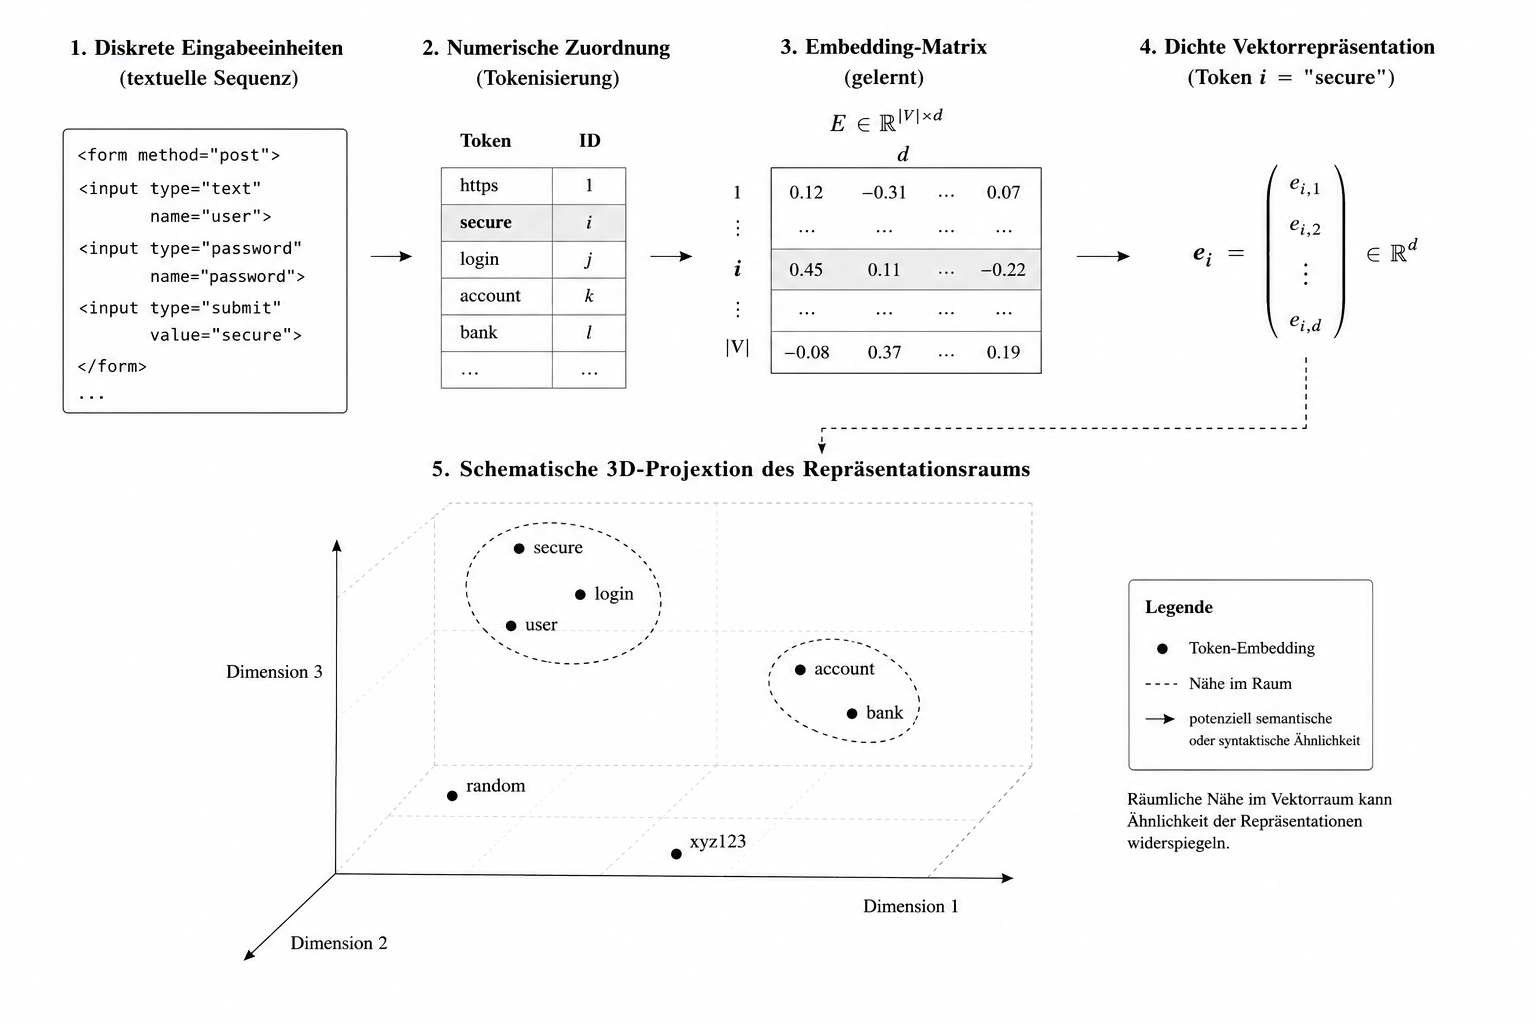
\includegraphics[width=\textwidth]
    {Praefix/Image/Vektorraum.png}

    \caption{Von diskreten Eingabeeinheiten zu gelernten Vektorrepräsentationen}
    \label{fig:vektorraum}
    \vspace{0.2em}

    {\footnotesize Quelle: (Eigene Darstellung nach [Collobert et al. (2011), S. 2501]; [Turney und Pantel (2010), S. 141 und 148]; [Mikolov et al. (2013), S. 1]); KI-unterstützt.}
\end{figure}

Die räumliche Anordnung in Abbildung~\ref{fig:vektorraum} verdeutlicht, dass
gelernte Vektorrepräsentationen über eine reine numerische Kennzeichnung
hinausgehen. Eine konzeptionelle Grundlage für die Interpretation
solcher Repräsentationsräume bildet die distributionelle Annahme, nach der
sprachliche Einheiten mit ähnlichen Verwendungskontexten tendenziell ähnliche
Bedeutungen aufweisen
(vgl. [Turney und Pantel (2010), S. 148]).
Auch gelernte Wortrepräsentationen können syntaktische und semantische Beziehungen
in ihren Vektoren abbilden
(vgl. [Mikolov et al. (2013), S. 1]).
Die dreidimensionale Darstellung in Abbildung \ref{fig:vektorraum} dient dabei
ausschließlich der schematischen Visualisierung eines tatsächlich
mehrdimensionalen Repräsentationsraums; die dargestellten Positionen und
Gruppierungen stellen keine empirisch ermittelten Repräsentationen des in dieser
Arbeit eingesetzten Modells dar.

Weitere parametrisierte Schichten können Eingaberepräsentationen schrittweise in höherstufige Merkmalsdarstellungen transformieren (vgl. [LeCun et al. (2015), S. 436]). Die Modellrepräsentation geht damit über die anfängliche Zuordnung eines Vektors zu einem Token hinaus.

Für die vorliegende Arbeit bildet dieses Prinzip die Grundlage für die Verarbeitung
der textuellen Eingabemodalitäten URL und HTML-Text. Die zusätzlich betrachtete
DOM-Struktur bildet demgegenüber explizite Beziehungen zwischen HTML-Elementen ab
und kann als Graph repräsentiert werden, in dem HTML-Elemente als Knoten und ihre
Eltern-Kind-Beziehungen als Kanten modelliert werden
(vgl. [Yoon et al. (2024), S. 9]). Neuronale und graphbasierte Verfahren zur
weiterführenden Repräsentationsbildung werden im folgenden Abschnitt betrachtet.

\subsection{Neuronale und graphbasierte Repräsentationsmodelle}

Neuronale Netze bestehen aus verbundenen Verarbeitungseinheiten mit trainierbaren Gewichten; verborgene Einheiten bilden interne Repräsentationen zwischen Ein- und Ausgabe (vgl. [Rumelhart et al. (1986), S.~533]).

Jede Einheit verarbeitet gewichtete Aktivierungen über eine Aktivierungsfunktion; die Gewichte werden anhand des Lernziels angepasst (vgl. [Rumelhart et al. (1986), S.~533]).

Deep Learning verbindet mehrere nichtlineare Verarbeitungsebenen, um geeignete Merkmale und aufeinander aufbauende Repräsentationen aus Daten zu erlernen (vgl. [Bengio (2009), S.~4--6]).


\begin{figure}[H]
    \centering

    \IfFileExists
    {Praefix/Image/NeuronaleNetze.png}
    {
        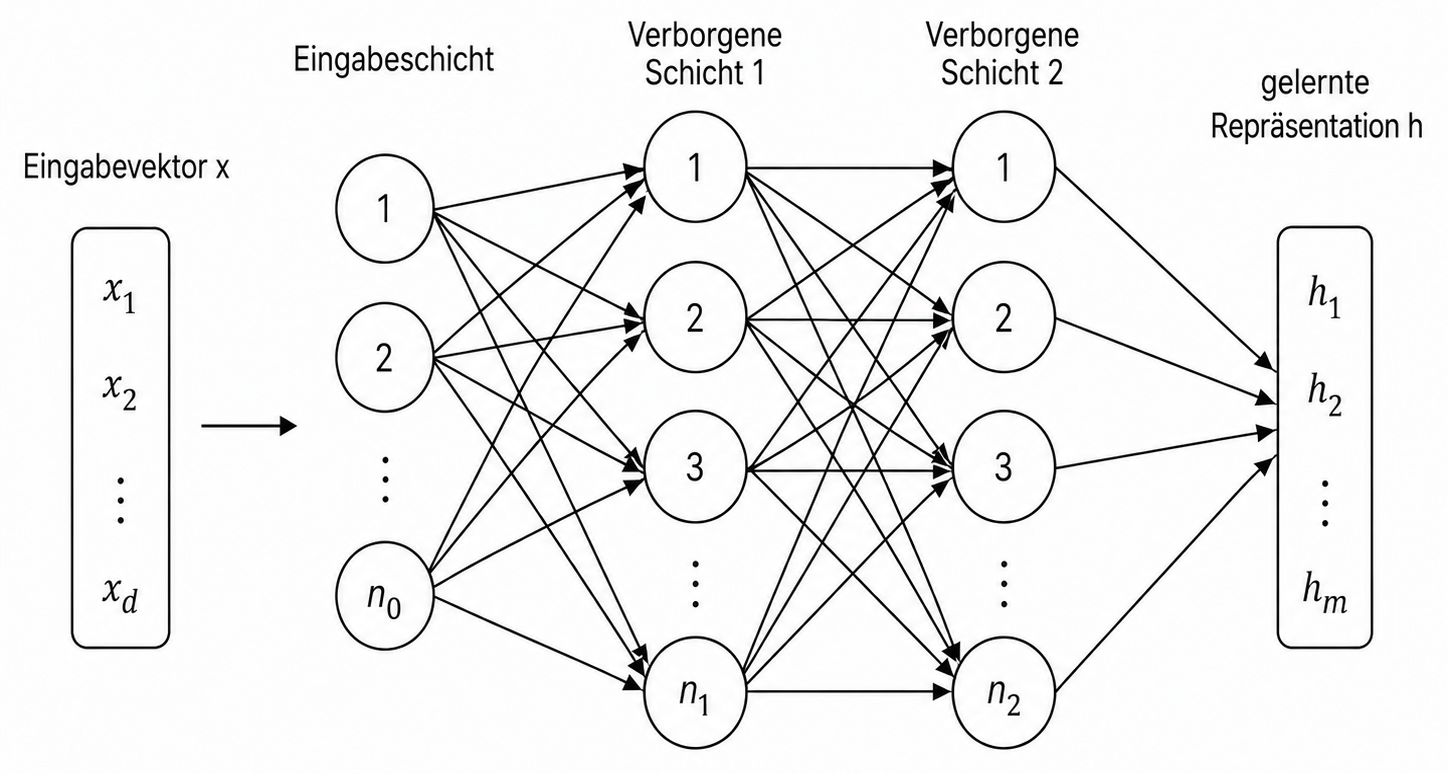
\includegraphics[width=\textwidth]
        {Praefix/Image/NeuronaleNetze.png}
    }
    {
        \fbox{
            \parbox[c][6.5cm][c]{0.92\textwidth}{
                \centering
                \textbf{Platzhalter Abbildung}\\[0.5em]
                Eingabevektor
                $\rightarrow$
                verborgene Schicht 1
                $\rightarrow$
                verborgene Schicht 2
                $\rightarrow$
                Ausgaberepräsentation
            }
        }
    }

    \caption{Schematischer Aufbau eines mehrschichtigen neuronalen Netzes}
    \label{fig:neuronale_repraesentationsbildung}
    \vspace{0.2em}

    {\footnotesize Quelle: (Eigene Darstellung nach [Rumelhart et al. (1986), S.~533]); KI-unterstützt.}
\end{figure}

Abbildung~\ref{fig:neuronale_repraesentationsbildung} zeigt eine vereinfachte mehrschichtige Verarbeitung. Zusätzliche verborgene Ebenen ermöglichen zunehmend abstrakte Merkmalsdarstellungen (vgl. [Bengio (2009), S. 4--6]).

Graphen ergänzen Knotenmerkmale um explizite Beziehungen zwischen den Knoten, die als Kanten dargestellt werden (vgl. [Kipf und Welling (2017), S. 1]).

Graph Convolutional Networks (GCNs) bilden Knotenrepräsentationen unter Berücksichtigung der eigenen Merkmale und der lokalen Nachbarschaft (vgl. [Kipf und Welling (2017), S. 1--2]). Mehrere Verarbeitungsschichten beziehen entsprechend weiter entfernte Nachbarschaften ein (vgl. [Kipf und Welling (2017), S. 3]).

Für Webseiten lässt sich dieses Prinzip auf die DOM-Struktur eines
HTML-Dokuments übertragen. HTML-Elemente können dabei als Knoten und ihre
hierarchischen Eltern-Kind-Beziehungen als Kanten eines Graphen modelliert
werden
(vgl. [Yoon et al. (2024), S. 9]).
Dadurch können neben den Eigenschaften einzelner HTML-Elemente auch deren
strukturelle Beziehungen in die Repräsentationsbildung einbezogen werden.

\begin{figure}[H]
    \centering
    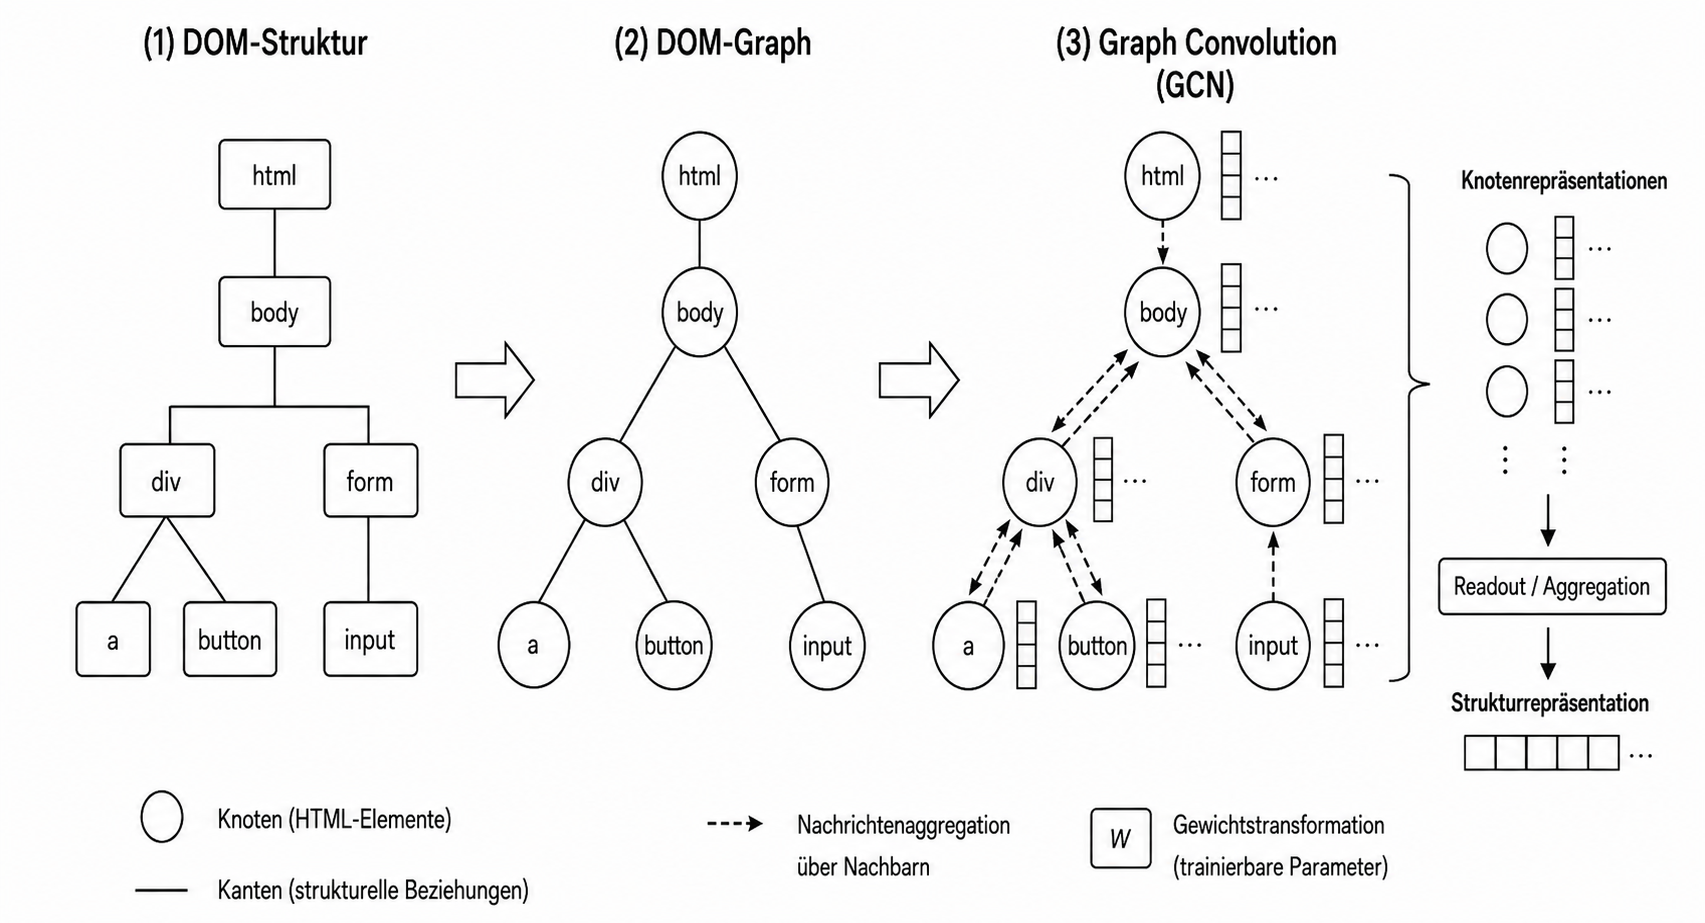
\includegraphics[
        width=1.0\textwidth,
        height=1.0\textheight,
        keepaspectratio
    ]{Praefix/Image/DOMDarstellung.png}
    \caption{Schematische graphbasierte Repräsentationsbildung einer DOM-Struktur}
    \label{fig:dom_gcn_repraesentationsbildung}
    \vspace{0.2em}

    {\footnotesize Quelle: (Eigene Darstellung nach [Kipf und Welling (2017), S. 1--3]; [Yoon et al. (2024), S. 9 und 13]); KI-unterstützt.}
\end{figure}

Abbildung \ref{fig:dom_gcn_repraesentationsbildung} veranschaulicht die
graphbasierte Verarbeitung dieser DOM-Struktur. Ein GCN kann dabei
Knotenmerkmale gemeinsam mit der lokalen Graphstruktur verarbeiten und daraus
strukturabhängige Repräsentationen erzeugen
(vgl. [Kipf und Welling (2017), S. 1--2]).

Damit stehen für die weitere Modellierung unterschiedliche Formen der
Repräsentationsbildung zur Verfügung. URL und HTML-Text werden als
sequenzielle Eingaben verarbeitet, während der DOM die explizite Struktur
des HTML-Dokuments graphbasiert abbildet. Für die kontextabhängige
Verarbeitung der sequenziellen Eingaben werden in der vorliegenden Arbeit
transformerbasierte Encodermodelle eingesetzt, die im folgenden Abschnitt
betrachtet werden.

\subsection{Transformerbasierte Repräsentationsmodelle}
\label{sec:transformerbasierte_repraesentationsmodelle}

Die ursprüngliche Transformer-Architektur besteht aus Encoder und Decoder; der Encoder überführt Eingabesequenzen in kontextabhängige Repräsentationen, die der Decoder für seine Ausgaben nutzt (vgl. [Vaswani et al. (2017), S. 2]). Da die Architektur ohne Rekurrenz und Faltung auskommt, werden den Embeddings Positionsinformationen hinzugefügt (vgl. [Vaswani et al. (2017), S. 6]).

Attention bildet Query-, Key- und Value-Vektoren und gewichtet Values anhand der Ähnlichkeit von Queries und Keys (vgl. [Vaswani et al. (2017), S. 3--4]). Für Scaled Dot-Product Attention gilt (vgl. [Vaswani et al. (2017), S. 4]):

\begin{equation*}
\mathrm{Attention}(Q,K,V)
=
\mathrm{softmax}
\left(
\frac{QK^{T}}{\sqrt{d_k}}
\right)V
\end{equation*}

\begin{center}
    \footnotesize{Quelle: (vgl. [Vaswani et al. (2017), S. 4]).}
\end{center}

\begin{description}
    \item[\textbf{$Q$ (Query):}]
    Repräsentiert die Anfragen, anhand derer bestimmt wird, welche
    Informationen anderer Sequenzpositionen für die jeweils betrachtete
    Position relevant sind.

    \item[\textbf{$K$ (Key):}]
    Enthält die Schlüsselrepräsentationen der Sequenzpositionen, mit denen
    die Queries zur Bestimmung ihrer jeweiligen Relevanz verglichen werden.

    \item[\textbf{$V$ (Value):}]
    Enthält die zu den Sequenzpositionen gehörenden Informationen, die
    entsprechend der berechneten Attention-Gewichte in die neue
    Repräsentation einfließen.

    \item[\textbf{$d_k$:}]
    Bezeichnet die Dimension der Key-Vektoren und dient als
    Skalierungsfaktor für die berechneten Skalarprodukte.
\end{description}

Die Skalarprodukte werden durch $\sqrt{d_k}$ skaliert, mittels Softmax normalisiert und zur gewichteten Kombination der Values verwendet (vgl. [Vaswani et al. (2017), S. 4]). Bei Self-Attention stammen Queries, Keys und Values aus derselben Sequenz (vgl. [Vaswani et al. (2017), S. 5]). Multi-Head Attention berechnet mehrere solcher Ausgaben mit eigenen Projektionen und führt sie anschließend zusammen (vgl. [Vaswani et al. (2017), S. 4--5]).

Im Encoder folgen auf Multi-Head Attention positionsweise Feed-Forward-Netze; beide Teilkomponenten besitzen Residualverbindungen und Layer-Normalisierung (vgl. [Vaswani et al. (2017), S. 3 und 5]).

Bidirectional Encoder Representations from Transformers (BERT) verwendet einen mehrschichtigen Transformer-Encoder, dessen Attention den Kontext auf beiden Seiten einer Tokenposition berücksichtigt (vgl. [Devlin et al. (2019), S. 4171 und 4173]). Für Klassifikation kann der abschließende Hidden State des speziellen Tokens \texttt{[CLS]} als Sequenzrepräsentation dienen (vgl. [Devlin et al. (2019), S. 4174]).

Neben der Feinabstimmung des Encoders beschreiben Devlin et al. einen feature-basierten Ansatz, bei dem extrahierte Aktivierungen als feste Merkmale nachgelagerter Modelle dienen (vgl. [Devlin et al. (2019), S. 4179]). Die vorliegende Arbeit nutzt diese Trennung für die Repräsentationsvergleiche.

RoBERTa verändert das BERT-Vortraining unter anderem durch umfangreicheres Training, größere Datenmengen, dynamische Maskierung und den Verzicht auf Next Sentence Prediction (vgl. [Liu et al. (2019), S. 1]). Abschnitt~2.3 erläutert die hier relevanten selbstüberwachten Lernziele.

In der vorliegenden Arbeit werden transformerbasierte Encoder für die
beiden sequenziellen Informationsquellen URL und HTML-Text eingesetzt.
Der URL-Zweig basiert auf BERT, während für den HTML-Text ein
RoBERTa-Encoder verwendet wird. Die daraus erzeugten
kontextabhängigen Repräsentationen bilden die Grundlage für die
nachfolgenden selbstüberwachten Repräsentationsvarianten und deren
kontrollierte Downstream-Evaluation.

\subsection{Downstream-Klassifikation und multimodale Verarbeitung}

Die Downstream-Aufgabe dieser Arbeit ist die überwachte Klassifikation einer Webseite als Phishing oder legitim. Eine Linear Probe trainiert einen linearen Klassifikator auf eingefrorenen Repräsentationen, um deren Nutzbarkeit zu bewerten (vgl. [Chen et al. (2020), PDF-S.~3]). Mehrschichtige Netze sind dagegen nicht auf lineare Entscheidungsregionen beschränkt; Cybenkos Approximationsresultat gilt dabei für ausreichend große Netze mit geeigneten sigmoiden Aktivierungen (vgl. [Cybenko (1989), S.~303]). Der empirische Vergleich mit einer nichtlinearen Probe prüft, wie stark die gemessenen Repräsentationsunterschiede vom Klassifikationsmechanismus abhängen.

Multimodale Fusion integriert Informationen mehrerer Modalitäten für eine gemeinsame Vorhersage; merkmalsbasierte Fusion verbindet Repräsentationen vor der Entscheidung, entscheidungsbasierte Fusion dagegen die Ausgaben getrennter Modelle (vgl. [Baltrušaitis et al. (2019), S.~12]). Für URL, HTML-Text und DOM wird hier eine merkmalsbasierte Fusion eingesetzt.

Lernbare Modalitätsgewichte können über Softmax normalisiert und zur gewichteten Summe der Repräsentationen verwendet werden (vgl. [Zhou et al. (2019), PDF-S. 1--2]). Andere Architekturen nutzen abweichende Gating-Funktionen, beispielsweise sigmoide Gated Multimodal Units (vgl. [Arevalo et al. (2017), S.~5]). Eine zusätzliche Entwurfsdimension ist die Kaskadierung: Frühe Stufen schließen einen Teil der Eingaben ab, während verbleibende Fälle aufwendigere Stufen durchlaufen (vgl. [Viola und Jones (2004), S.~144]).



\section{Self-Supervised Representation Learning}
Self-Supervised Representation Learning leitet Trainingsziele aus den Eingabedaten selbst ab; eine solche Hilfsaufgabe (\textit{Pretext Task}) benötigt keine manuell annotierten Zielwerte der späteren Aufgabe (vgl. [Ericsson et al. (2022), S. 42--43]). Die vortrainierten Repräsentationen können anschließend als feste Merkmale oder durch weitere Feinabstimmung für eine \textit{Downstream Task} genutzt werden (vgl. [Ericsson et al. (2022), S. 44--45]).

Abbildung \ref{fig:ssrl_grundprinzip} veranschaulicht diese Trennung
zwischen selbstüberwachtem Vortraining und nachgelagerter Nutzung der
erlernten Repräsentationen.

\begin{figure}[H]
    \centering

    \begin{tikzpicture}[
        font=\footnotesize,
        >={Latex[length=2.1mm]},
        topbox/.style={
            draw=black,
            line width=0.55pt,
            align=center,
            text width=3.1cm,
            minimum height=2.9cm,
            inner sep=4pt
        },
        box/.style={
            draw=black,
            line width=0.55pt,
            align=center,
            text width=3.1cm,
            minimum height=1.9cm,
            inner sep=4pt
        },
        arrow/.style={
            ->,
            line width=0.65pt
        },
        node distance=0.6cm
    ]

    % Obere Reihe
    \node[topbox] (data) {
        \textbf{Ungelabelte Daten}\\[3pt]
        z.\,B. Texte, Webseiten\\
        oder Dokumente
    };

    \node[topbox, right=of data] (pretext) {
        \textbf{Selbstüberwachtes}\\
        \textbf{Lernziel}\\
        \textit{(Pretext Task)}\\[3pt]
        z.\,B. Maskierung oder\\
        kontrastive Paarung
    };

    \node[topbox, right=of pretext] (encoder) {
        \textbf{Encoder / Vortraining}\\[3pt]
        Lernen einer\\
        übertragbaren\\
        Repräsentations-\\
        funktion
    };

    % Untere Reihe
    \node[
        box,
        below=0.75cm of encoder
    ] (representation) {
        \textbf{Gelernte}\\
        \textbf{Repräsentation}\\[3pt]
        Übertragbare\\
        Merkmalsdarstellung
    };

    \node[
        box,
        right=of representation
    ] (downstream) {
        \textbf{Downstream-Aufgabe}\\
        \textit{(mit Labels)}\\[3pt]
        z.\,B. Klassifikation
    };

    % Pfeile
    \draw[arrow] (data.east) -- (pretext.west);
    \draw[arrow] (pretext.east) -- (encoder.west);
    \draw[arrow] (encoder.south) -- (representation.north);
    \draw[arrow] (representation.east) -- (downstream.west);

    \end{tikzpicture}

    \caption{Grundprinzip des Self-Supervised Representation Learning}
    \label{fig:ssrl_grundprinzip}
    \vspace{0.2em}

    {\footnotesize Quelle: (Eigene Darstellung nach [Ericsson et al. (2022), S. 42--46]); KI-unterstützt.}
\end{figure}

Die Wahl der Pretext-Aufgabe bestimmt das Trainingssignal und beeinflusst die erlernte Repräsentation (vgl. [Ericsson et al. (2022), S. 42--43]). Im Folgenden werden maskierte und kontrastive Lernziele sowie die task-adaptive Weiteranpassung unterschieden.

\subsection{Maskierte selbstüberwachte Lernziele}

Masked Language Modeling (MLM) trainiert einen Encoder darauf, ausgewählte Token aus dem verbleibenden beidseitigen Kontext zu rekonstruieren; die ursprünglichen Token liefern dabei die Zielwerte ohne manuelle Klassenannotation (vgl. [Devlin et al. (2019), S.~4172 und 4174]).

BERT wählt 15~\% der Tokenpositionen aus, ersetzt davon 80~\% durch das Maskierungstoken und 10~\% durch zufällige Token und belässt 10~\% unverändert; für diese Positionen wird jeweils das ursprüngliche Token vorhergesagt (vgl. [Devlin et al. (2019), S.~4174]). Auch RoBERTa nutzt MLM als Vortrainingsziel (vgl. [Gururangan et al. (2020), S.~8343]).

Das grundlegende Zusammenspiel aus Maskierung, kontextabhängiger
Repräsentationsbildung und Rekonstruktion ist in Abbildung~\ref{fig:mlm-konzept}
exemplarisch für eine HTML-Textsequenz dargestellt.

\begin{figure}[H]
    \centering
    % KI-unterstuetzte eigene schematische Darstellung; keine gemessenen Tokenfolgen.
\begin{tikzpicture}[font=\small,>=stealth,
  box/.style={draw,rounded corners=2pt,align=center,minimum height=.8cm,text width=11cm}]
\node[box] (input) {Bereinigter HTML-Text: \texttt{Secure Login -- Verify your account}};
\node[box,above=0.5cm of input] (masked) {Maskierte Eingabe: \texttt{<mask> Login -- Verify your <mask>}};
\node[box,above=0.5cm of masked] (encoder) {RoBERTa-Encoder: kontextabhängige Tokenrepräsentationen};
\node[box,above=0.5cm of encoder] (head) {MLM-Head: Vorhersage der ursprünglichen ausgewählten Token};
\node[above=0.35cm of head,align=center] (target) {Schematische Vorhersageziele: \texttt{Secure}, \texttt{account}};
\draw[->] (input)--(masked);
\draw[->] (masked)--(encoder);
\draw[->] (encoder)--(head);
\draw[->] (head)--(target);
\end{tikzpicture}

    \caption{Schematisches Prinzip des Masked Language Modeling am Beispiel des HTML-Textzweigs}
    \label{fig:mlm-konzept}
    \vspace{0.2em}

    {\footnotesize Quelle: (Eigene Darstellung nach [Devlin et al. (2019), S.~4174]; [Gururangan et al. (2020), S.~8343]); KI-unterstützt.}
\end{figure}

Abbildung~\ref{fig:mlm-konzept} überträgt MLM auf den HTML-Textzweig. Die Wörter sind schematisch; im Code werden Subword-Token maskiert und rekonstruiert. MLM kann auch das Vortraining auf weiteren ungelabelten Daten fortsetzen (vgl. [Gururangan et al. (2020), S.~8343]). Abschnitt~2.3.3 behandelt die aufgabenbezogene Fortsetzung.

\subsection{Kontrastives Repräsentationslernen}

Kontrastives Lernen nähert Repräsentationen positiver Paare einander an und unterscheidet sie von negativen Vergleichsinstanzen; für Text kann dies mit vortrainierten Transformer-Encodern umgesetzt werden (vgl. [Gao et al. (2021), S.~6895]).

Die Ähnlichkeit zweier Repräsentationen kann dabei über die
Kosinusähnlichkeit bestimmt werden. Innerhalb der kontrastiven
Verlustfunktion beeinflusst ein Temperaturparameter die Skalierung der
Ähnlichkeitswerte. Das Lernziel begünstigt dadurch eine hohe Ähnlichkeit
positiver Paare relativ zu den verfügbaren negativen Vergleichsinstanzen
(vgl. [Gao et al. (2021), S.~6895]).
\begin{figure}[H]
    \centering
    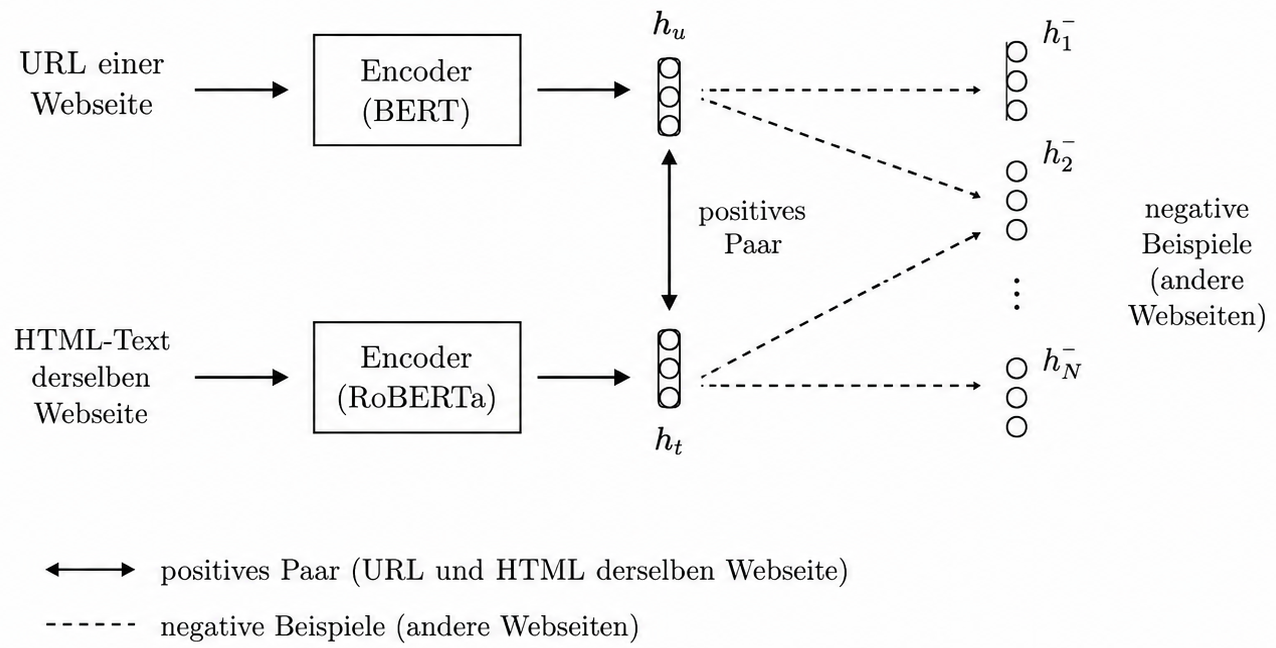
\includegraphics[width=0.72\textwidth]{Praefix/Image/ContrastiveKonzept.png}
    \caption{Schematisches Prinzip des kontrastiven Repräsentationslernens für URL--HTML-Paare}
    \label{fig:contrastive-konzept}
    \vspace{0.2em}

    {\footnotesize Quelle: (Eigene Darstellung nach [Gao et al. (2021), S.~6895]); Übertragung auf URL--HTML-Paare, KI-unterstützt.}
\end{figure}

Ergänzend wird kontrastives Repräsentationslernen als alternative
selbstüberwachte Zielfunktion betrachtet. URL und HTML-Text derselben Webseite
bilden dabei ein positives Paar, während Repräsentationen anderer Webseiten als
negative Beispiele dienen. Das Trainingssignal entsteht somit ohne Verwendung
von Phishing- oder Benign-Labels. Die konkrete Umsetzung wird in
Abschnitt~4.3.2 beschrieben.

\subsection{Task-Adaptive Pretraining}

Task-Adaptive Pretraining (TAPT) setzt das RoBERTa-Vortraining auf dem ungelabelten Trainingskorpus einer konkreten Downstream-Aufgabe fort (vgl. [Gururangan et al. (2020), S. 8346]).

Die angepassten Repräsentationen werden anschließend für das überwachte Training der Zielaufgabe verwendet (vgl. [Gururangan et al. (2020), S. 8346]).

Die Trennung beider Lernphasen lässt sich vereinfacht wie folgt darstellen:

\begin{equation}
\theta_{\mathrm{pre}}
\xrightarrow[\mathcal{D}^{\mathrm{unlabeled}}_{\mathrm{task}}]
{\mathcal{L}_{\mathrm{MLM}}}
\underbrace{\theta_{\mathrm{TAPT}}}_{\text{Task-Adaptive Pretraining}}
\rightarrow
\theta_{\mathrm{TAPT}}
\xrightarrow[\mathcal{D}^{\mathrm{labeled}}_{\mathrm{task}}]
{\mathcal{L}_{\mathrm{cls}}}
\underbrace{\theta_{\mathrm{task}}}_{\text{Downstream-Training}} .
\end{equation}

\begin{center}
    \footnotesize{Quelle: (Eigene Darstellung nach [Gururangan et al. (2020), S.~8346]); KI-unterstützt.}
\end{center}

Domain-Adaptive Pretraining (DAPT) nutzt dagegen einen breiteren ungelabelten Korpus der Domäne; TAPT ist durch die Auswahl der Trainingsdaten enger an eine konkrete Zielaufgabe gebunden (vgl. [Gururangan et al. (2020), S. 8342--8343 und 8346]).

In der vorliegenden Arbeit wird TAPT auf die beiden sequenziellen Informationsquellen URL und
HTML-Text übertragen. Die vortrainierten Encoder werden hierzu getrennt mittels MLM auf dem
ungelabelten Webseiten-Trainingspool weiter angepasst. Da derselbe Pool anschließend die
Ausgangsbasis der gelabelten Downstream-Budgets bildet, entspricht dieser Versuchsaufbau der
task-adaptiven Variante. Dadurch lassen sich die isolierte Anpassung einzelner
Informationsquellen sowie ihre gemeinsame Anpassung gegenüber nicht adaptierten
Repräsentationen unter unterschiedlichen Labelbudgets und Evaluationsbedingungen untersuchen.
\section{Evaluationsrahmen und Bewertungsmetriken}
\label{sec:evaluation_metrics}

\subsection{Klassifikations- und Betriebspunktmetriken}

\paragraph{True-Positive-Rate, False-Positive-Rate und Precision}
Bei einer binären Klassifikation ergeben sich aus tatsächlicher und vorhergesagter Klasse
die vier Fälle True Positive (TP), False Positive (FP), True Negative (TN) und False
Negative (FN). Darauf aufbauend lassen sich True-Positive-Rate (TPR),
False-Positive-Rate (FPR) und Precision bestimmen
(vgl. [Saito und Rehmsmeier (2015), S. 3--4]):

\[
\mathrm{TPR}=\frac{TP}{TP+FN},
\qquad
\mathrm{FPR}=\frac{FP}{FP+TN},
\qquad
\mathrm{Precision}=\frac{TP}{TP+FP}.
\]

\begin{center}
\footnotesize Quelle: (vgl. [Saito und Rehmsmeier (2015), S. 4]).
\end{center}

TPR entspricht dem Recall, FPR dem Anteil falsch positiver unter allen negativen Instanzen und Precision dem Anteil tatsächlich positiver unter allen positiven Vorhersagen (vgl. [Saito und Rehmsmeier (2015), S. 4]). In dieser Arbeit ist Phishing die positive und legitim die negative Klasse.

\paragraph{Betriebspunkt} Die Klassifikationsschwelle bestimmt das Verhältnis von TPR und FPR (vgl. [Saito und Rehmsmeier (2015), S. 4]). Für die Phishing-Erkennung sind insbesondere Betriebspunkte mit niedriger FPR relevant (vgl. [Purwanto et al. (2022), S. 1506]).

Die vorliegende Arbeit betrachtet deshalb primär die TPR an einem festgelegten
Low-FPR-Betriebspunkt und die dort realisierte FPR. Ergänzend wird mit
$\mathrm{FPR@TPR90}$ die umgekehrte Perspektive verwendet: Sie gibt an, welche
False-Positive-Rate am ersten empirischen ROC-Punkt mit einer TPR von mindestens
90\,\% erreicht wird. Eine Interpolation auf exakt 90\,\% erfolgt nicht.
Niedrigere Werte entsprechen dabei einer günstigeren Trennung der beiden Klassen.
Beide Perspektiven erlauben damit eine Bewertung der Klassifikationsleistung bei
kontrollierter Erkennungs- beziehungsweise Fehlalarmrate.

\paragraph{Ergänzende Precision-Recall-Metriken}
Neben einzelnen Betriebspunkten kann die Modellleistung über unterschiedliche
Klassifikationsschwellen betrachtet werden. Die Precision-Recall-Kurve stellt hierzu
Precision und Recall über verschiedene Schwellenwerte gegenüber
(vgl. [Saito und Rehmsmeier (2015), S. 4 und 7]). Die Average Precision (AP) fasst
diese Rankingperspektive über die Kurve zusammen. Dalton et al. verwenden im
PhreshPhish-Benchmark ergänzend eine als Precision bei 90\,\% Recall bezeichnete
Kennzahl ($P@R=0{,}90$) (vgl. [Dalton et al. (2026), S. 7]).

Precision und darauf aufbauende Precision-Recall-Metriken hängen zusätzlich von der
Klassenverteilung der Evaluationsmenge ab
(vgl. [Saito und Rehmsmeier (2015), S. 5 und 7]). AP und der nachfolgend präzisierte
Kennwert $P_{\geq 90}$ werden in der
vorliegenden Arbeit daher ergänzend zur Beschreibung der Rankingqualität auf einem
festen Evaluationsbestand verwendet. Die zentralen Modell- und Systemvergleiche
stützen sich dagegen auf TPR und FPR an den festgelegten Betriebspunkten.
Der implementierte Kennwert $P_{\geq 90}$ ist die maximale Precision unter allen
empirischen Schwellen mit Recall von mindestens 90\,\%:
\[
P_{\geq 90}=\max_{\tau:\,\mathrm{TPR}(\tau)\geq 0{,}90}
\mathrm{Precision}(\tau).
\]
Er bezeichnet somit keine interpolierte Precision bei exakt 90\,\% Recall.
AP wird als Summe der Precision-Werte gewichtet mit den jeweiligen Recall-Zuwächsen
berechnet; sie entspricht hier keiner trapezförmigen Flächenintegration.


\subsection{Generalisierung unter Distribution Shift}

Eine besondere Herausforderung für die Generalisierung lernbasierter Modelle
entsteht, wenn sich die zugrunde liegende Datenverteilung zwischen Training und
späterer Evaluation verändert. Koh et al. bezeichnen als Distribution Shift
Situationen, in denen sich Trainings- und Testverteilung unterscheiden
(vgl. [Koh et al. (2021), PDF-S. 1]). Vereinfacht lässt sich dieser Zusammenhang
durch

\[
P_{\mathrm{train}}(X,Y) \neq P_{\mathrm{test}}(X,Y)
\]

beschreiben, wobei \(X\) die Eingabedaten und \(Y\) die zugehörige Zielklasse
bezeichnet. Koh et al. zeigen anhand mehrerer realer Datensätze, dass Modelle
unter solchen Out-of-Distribution-Bedingungen deutlich geringere Leistungen
als unter vergleichbaren Trainings- und Testbedingungen erreichen können
(vgl. [Koh et al. (2021), PDF-S. 1--2]).

Zeitliche Veränderungen und zuvor unbeobachtete Domänen bilden mögliche Ursachen von Verteilungsverschiebungen; WILDS berücksichtigt beide Formen in seinen Testbedingungen (vgl. [Koh et al. (2021), PDF-S.~1--3]).

Für die vorliegende Arbeit bildet diese Unterscheidung die theoretische
Grundlage für die spätere Evaluation unter veränderten Datenbedingungen.
Die konkrete Konstruktion der verwendeten Testszenarien und die Festlegung des
Low-FPR-Betriebspunkts werden in Abschnitt~4.4.1 beschrieben.

\subsection{Statistische Auswertungsverfahren}

Stochastisches Training kann zwischen Läufen unterschiedliche Ergebnisse erzeugen; Reimers und Gurevych empfehlen deshalb die Bewertung mehrerer Ausführungen anstelle einzelner Ergebniswerte (vgl. [Reimers und Gurevych (2017), S.~338]).

\paragraph{Gepaarte Leistungsdifferenzen}
Werden zwei Modellvarianten unter korrespondierenden Bedingungen verglichen,
können die jeweils zusammengehörigen Beobachtungen paarweise gegenübergestellt
werden. Holt und Sullivan bilden hierfür die Differenzen zwischen den
Beobachtungspaaren und verwenden deren Mittelwert als Teststatistik
(vgl. [Holt und Sullivan (2023), S.~787--788]):

\begin{equation*}
d_i=x_i-y_i,
\qquad
T=\bar{d}.
\end{equation*}

\begin{center}
    \footnotesize{Quelle: (vgl. [Holt und Sullivan (2023), S.~787--788]).}
\end{center}

Die Paarbildung erhält die Zuordnung korrespondierender Beobachtungen (vgl. [Holt und Sullivan (2023), S.~787--788]). Differenzen prozentual ausgewiesener Metriken werden in dieser Arbeit in Prozentpunkten berichtet.

\paragraph{Konfidenzintervalle} Konfidenzintervalle ergänzen Punktschätzungen um eine Unsicherheitsangabe, häufig zum Niveau von 95~\% oder 99~\% (vgl. [Botsch (2023), S. 15]). Hier beschreiben 95-\%-Intervalle die Unsicherheit mittlerer Differenzen aus gepaarten Downstream-Wiederholungen; ihre Interpretation setzt die in Kapitel~4 genannten Bedingungen voraus.

Bootstrap-Resampling zieht wiederholt Stichproben gleicher Größe mit Zurücklegen und berechnet die Leistungsmetrik erneut (vgl. [Raschka (2018), S. 16]). Beim 95-\%-Percentile-Intervall bilden das 2,5-\%- und 97,5-\%-Quantil der Bootstrap-Verteilung die Grenzen (vgl. [Raschka (2018), S. 18]).

\paragraph{Exakter Sign-Flip-Permutationstest} Bei unter der Nullhypothese um null symmetrischen Paardifferenzen lässt sich eine Nullverteilung ihres Mittelwerts durch alle Vorzeichenkombinationen bilden (vgl. [Holt und Sullivan (2023), S. 787--788]).

Für $n$ Paare gibt es $2^n$ Vorzeichenkombinationen; der zweiseitige exakte $p$-Wert ist deren Anteil mit einem mindestens so großen absoluten Mittelwert wie beobachtet (vgl. [Holt und Sullivan (2023), S. 788]).

\paragraph{Korrektur multipler Tests} Mit mehreren Hypothesentests kann das Risiko mindestens einer falschen Zurückweisung innerhalb der Testfamilie steigen (vgl. [Dror et al. (2017), S.~471 und 474]).

Die Holm-Prozedur sortiert $m$ $p$-Werte aufsteigend und vergleicht sie nacheinander mit $\alpha/(m-i+1)$, bis erstmals keine Zurückweisung erfolgt; dadurch wird die familienbezogene Fehlerwahrscheinlichkeit kontrolliert (vgl. [Holm (1979), S.~66--67]).

In der vorliegenden Arbeit werden die Größenordnung der beobachteten
Leistungsunterschiede, die Unsicherheit ihrer Schätzung und die Ergebnisse der
statistischen Tests gemeinsam berichtet. Die konkrete Anzahl der Wiederholungen,
die Paarbildung sowie die Zuordnung mehrerer Vergleiche zu gemeinsamen
Testfamilien werden im Methodikkapitel festgelegt.

\subsection{Effizienz- und Betriebsmetriken}

Die technische Evaluation berücksichtigt neben der Klassifikationsgüte auch den Inferenzaufwand. Reddi et al. unterscheiden latenzorientierte Szenarien und durchsatzorientierte Batch-Verarbeitung (vgl. [Reddi et al. (2020), S.~5--6]).

\begin{itemize}
    \item \textbf{Median-Latenz [ms]:}
    bezeichnet in dieser Arbeit das 50.\ Perzentil der gemessenen
    Inferenzzeiten und beschreibt damit die typische Verarbeitungsdauer
    einer Eingabe.

    \item \textbf{95.\ Perzentil der Latenz [ms]:}
    bezeichnet den Latenzwert, den 95\,\% der beobachteten
    Inferenzvorgänge nicht überschreiten. Perzentilbasierte
    Latenzmetriken werden auch in etablierten Inferenzbenchmarks zur
    Betrachtung langsamerer Bereiche der Laufzeitverteilung eingesetzt
    (vgl. [Reddi et al. (2020), S.~5--6]).

    \item \textbf{Durchsatz [Seiten/s]:}
    beschreibt die Anzahl der innerhalb eines Zeitraums verarbeiteten
    Eingaben. Im Offline-Szenario des MLPerf-Inference-Benchmarks wird
    entsprechend der Durchsatz in Samples pro Sekunde betrachtet
    (vgl. [Reddi et al. (2020), S.~6]).

    \item \textbf{Peak-VRAM [MiB]:}
    bezeichnet in dieser Arbeit den maximal während des betrachteten
    Inferenzpfads belegten GPU-Speicher.

    \item \textbf{Eskalationsrate [\%]:}
    bezeichnet bei einer kaskadierten Verarbeitung den Anteil der Eingaben,
    für die nach der ersten Verarbeitungsstufe zusätzlich der vollständige
    multimodale Modellpfad ausgeführt wird.
\end{itemize}

Latenz und Durchsatz erfassen unterschiedliche Aspekte der technischen
Verarbeitung und sind daher gemeinsam zu betrachten
(vgl. [Reddi et al. (2020), S.~11]). Peak-VRAM und Eskalationsrate ergänzen
diese Kennzahlen um den Ressourcenbedarf und den Verarbeitungsumfang.


\chapter{Stand der Forschung und Forschungslücke}

\section{Task-adaptive Repräsentationen und Label-Effizienz}

Ein Forschungsstrang der Phishing-Erkennung untersucht, wie transformerbasierte
Repräsentationen bereits vor der gelabelten Zielklassifikation an Web- und insbesondere
URL-Daten angepasst werden können. URLTran vergleicht zwei Ansätze: ausschließlich
auf URLs vortrainierte und anschließend feinabgestimmte Transformer sowie die direkte
Feinabstimmung öffentlich vortrainierter BERT- und RoBERTa-Modelle. Die Evaluation
berücksichtigt gezielt Betriebspunkte mit sehr niedrigen False-Positive-Raten
(vgl. [Maneriker et al. (2021), PDF-S. 1--2]). PhishBERT wird auf mehr als drei Milliarden
ungelabelten URLs vortrainiert und anschließend für die Phishing-Klassifikation
weiterverwendet (vgl. [Wang et al. (2023), Abstract, o.\,S.]). Auch urlBERT nutzt mehrere Milliarden
URLs und kombiniert mehrere selbstüberwachte Vortrainingsziele; ergänzend wird die
Sensitivität gegenüber reduziertem gelabeltem Trainingsumfang untersucht
(vgl. [Li et al. (2025), S. 1--2 und 12]).

Neben der domänennäheren Repräsentationsbildung rückt damit die verfügbare gelabelte
Downstream-Supervision in den Fokus. Gui et al. führen den Aufwand der Erhebung und
Annotation großer gelabelter Datenbestände als eine Motivation für Self-Supervised Learning
an (vgl. [Gui et al. (2024), S. 1]). Für spezialisierte URL-Repräsentationen untersuchen
Li et al. ergänzend, wie sich die Downstream-Leistung bei reduziertem gelabeltem
Trainingsumfang verändert (vgl. [Li et al. (2025), S. 12]).

Für die vorliegende Arbeit sind daraus zwei Aspekte relevant. Erstens wird untersucht,
welchen zusätzlichen Nutzen die in Abschnitt 2.3.3 eingeführte task-adaptive
Weiteranpassung bereits vortrainierter URL- und HTML-Text-Encoder für die
Phishing-Klassifikation erzeugt. Durch die getrennte und gemeinsame Anpassung beider
Informationszweige wird zugleich betrachtet, wie sich dieser Effekt zwischen URL und
HTML-Text verteilt. Zweitens wird die gelabelte Downstream-Supervision systematisch
über mehrere Labelbudgets variiert, um zu bestimmen, wie sich der
Repräsentationsvorteil mit wachsendem Trainingsumfang entwickelt und ab welchem
reduzierten Labelbudget das festgelegte Leistungsniveau vollständig trainierter
Referenzen erreicht wird.

\section{Informationsgrundlage und Systemarchitektur}

Neben der Repräsentationsbildung unterscheiden sich bestehende Verfahren hinsichtlich
der für die Klassifikation verwendeten Webseiteninformationen. Aljofey et al. kombinieren
URL-Zeichenfolgen, Hyperlinkinformationen und textuelle HTML-Merkmale und führen diese
einem XGBoost-Klassifikator zu
(vgl. [Aljofey et al. (2022), S. 1--2 und 13]). Opara et al. verarbeiten URL- und
HTML-Informationen dagegen in einem gemeinsamen neuronalen Verfahren
(vgl. [Opara et al. (2024), S. 2]). Damit werden URL und HTML-Inhalt als unterschiedliche
Informationsquellen derselben Webseite für die Klassifikation nutzbar gemacht.

Über den textuellen HTML-Inhalt hinaus kann auch die Dokumentstruktur berücksichtigt
werden. Yoon et al. kombinieren URL-Repräsentationen mit einem graphbasierten
HTML-DOM und untersuchen den zusätzlichen Beitrag der strukturellen Information anhand
von Ablationen (vgl. [Yoon et al. (2024), S. 2, 13 und 15]). Die bestehende Forschung
liefert damit eine Grundlage dafür, adressbezogene, textuelle und strukturelle
Informationen innerhalb eines gemeinsamen Klassifikationssystems zu berücksichtigen.

Die vorliegende Arbeit trennt dabei Repräsentations- und Systemebene. Zunächst wird die
task-adaptive URL- und HTML-Text-Repräsentation unter konstant gehaltenen
Downstream-Bedingungen untersucht. Die daraus ausgewählte Repräsentationsbasis wird
anschließend schrittweise um weitere Systemkomponenten erweitert. Eine sequenzielle
Ablation von URL über HTML-Text und DOM bis zur lernbaren Gating-Fusion bestimmt
hierbei den inkrementellen Beitrag der zusätzlichen Informations- und
Fusionskomponenten.

Neben dem Informationsumfang kann auch die Verarbeitungstiefe Bestandteil des
Systementwurfs sein. Liu et al. beschreiben ein mehrstufiges
Phishing-Erkennungsverfahren und berichten eine Verkürzung der Ausführungszeit
bei zugleich verbesserter Erkennung
(vgl. [Liu et al. (2021), Abstract, o.\,S.]). Dieses Prinzip bildet den konzeptionellen
Bezug für die URL-first-Kaskade der vorliegenden Arbeit. Die URL-Stufe dient dabei
als vorgelagerter Entscheidungspfad, während für unsichere Fälle weiterhin das
vollständige multimodale System ausgeführt wird.

\section{Generalisierung und betriebliche Evaluationsbedingungen}

Die Aussagekraft eines Phishing-Klassifikators hängt neben der Modellarchitektur auch
von der Zusammensetzung der Evaluationsdaten ab. Rashid et al. untersuchen
URL-Klassifikatoren über unterschiedliche Datensätze hinweg und berichten deutliche
Leistungsunterschiede zwischen datensatzinternen und datensatzübergreifenden
Evaluationen (vgl. [Rashid et al. (2024), Abstract, o.\,S.]). Dalton et al. adressieren im
PhreshPhish-Benchmark eine verwandte Problematik durch zeitlich getrennte Trainings-
und Testdaten sowie eine zusätzliche Reduktion stark ähnlicher Instanzen
(vgl. [Dalton et al. (2026), S. 5--6]).

Für die vorliegende Untersuchung wird die Leistungsrelation zwischen den
Repräsentationsvarianten und Labelbudgets deshalb nicht ausschließlich auf dem
vollständigen Testbestand betrachtet. Ergänzende domain-, template- und zeitbezogene
Teilmengen bilden zusätzliche Evaluationsbedingungen. Sie dienen der Prüfung, ob die
zuvor beobachteten Repräsentations- und Budgetrelationen auch unter veränderter
Zusammensetzung der Testdaten bestehen bleiben.

Eine weitere Evaluationsdimension bildet der Klassifikationsbetriebspunkt. URLTran
untersucht seine Modelle gezielt bei niedrigen False-Positive-Raten
(vgl. [Maneriker et al. (2021), PDF-S. 1--2]). Auch im operativen Sicherheitsbetrieb
werden False-Positive-Raten gemeinsam mit Größen wie Eskalationen und
Bearbeitungsaufwand als Qualitätskennzahlen betrachtet
(vgl. [ENISA (2020), S. 7]). Die vorliegende Arbeit verwendet daher einen auf einer
getrennten Kalibrationsmenge bestimmten Low-FPR-Betriebspunkt, der anschließend
unverändert auf die finalen Evaluationsbedingungen übertragen wird.

Für die technische Bewertung des Gesamtsystems kommen Ressourcenkennzahlen der
Inferenz hinzu. Reddi et al. unterscheiden insbesondere latenz- und
durchsatzorientierte Inferenzszenarien
(vgl. [Reddi et al. (2020), S. 5--6]). Entsprechend werden neben der
Klassifikationsleistung auch Latenz, Durchsatz, GPU-Speicherbedarf und
Eskalationsrate betrachtet.

\section{Forschungslücke und Einordnung der Arbeit}

Die betrachteten Forschungsarbeiten adressieren die für diese Arbeit relevanten
Aspekte überwiegend auf einzelnen Ebenen. Spezialisierte selbstüberwachte
URL-Repräsentationen zeigen die Nutzbarkeit domänennäherer Repräsentationsbildung;
Untersuchungen reduzierter Labelmengen betrachten die Downstream-Leistung bei
begrenzter Supervision. Weitere Arbeiten kombinieren mehrere Webseiteninformationen
oder verwenden mehrstufige Klassifikationsarchitekturen.

Aus dieser Ausgangslage ergibt sich für die vorliegende Arbeit die Verbindung dreier
Untersuchungsebenen. Zunächst wird der zusätzliche Effekt einer task-adaptiven
Weiteranpassung bereits vortrainierter URL- und HTML-Text-Repräsentationen isoliert.
Darauf aufbauend wird untersucht, wie sich dieser Effekt über unterschiedliche
Labelbudgets entwickelt und ab welchem reduzierten Budget das festgelegte
Leistungsniveau vollständig trainierter Referenzen erreicht wird. Die ausgewählte
Repräsentationsbasis wird anschließend in ein multimodales Gesamtsystem überführt,
dessen zusätzliche Komponenten und gestufte Verarbeitung getrennt evaluiert werden.

Tabelle~\ref{tab:forschungsableitung} fasst die für das Untersuchungsdesign
maßgeblichen Forschungsbezüge zusammen.

\begin{table}[!ht]
\centering
\caption{Einordnung des Untersuchungsdesigns in den Stand der Forschung.}
\label{tab:forschungsableitung}

\footnotesize
\setlength{\tabcolsep}{4pt}
\renewcommand{\arraystretch}{1.08}

\begin{tabular}{@{}>{\raggedright\arraybackslash}p{3.7cm}>{\raggedright\arraybackslash}p{4.5cm}>{\raggedright\arraybackslash}p{5.0cm}@{}}
\toprule
\textbf{Forschungsbereich}
&
\textbf{Bezug zur vorliegenden Arbeit}
&
\textbf{Umsetzung}
\\
\midrule

Selbstüberwachte URL-Repräsentationen
(vgl. [Maneriker et al. (2021), PDF-S. 1--2]; [Wang et al. (2023), Abstract, o.\,S.]; [Li et al. (2025), S. 1--2 und 12])
&
Zusätzliche task-adaptive Anpassung bereits vortrainierter URL- und
HTML-Text-Repräsentationen.
&
Vergleich von R0, RU, RT und RUT bei konstanten Downstream-Probes.
\\[1mm]

Nutzung ungelabelter Daten und reduzierte Labelbudgets
(vgl. [Gui et al. (2024), S. 1]; [Li et al. (2025), S. 1--2 und 12])
&
Verhalten der Repräsentationsvarianten bei unterschiedlicher gelabelter
Downstream-Supervision.
&
Sieben Labelbudgets sowie Bestimmung der kleinsten ausreichenden
RUT-Stufe gegenüber vollständig mit 200.000 Labels trainierten Referenzen.
\\[1mm]

Mehrquellenbasierte Webseitenklassifikation
(vgl. [Aljofey et al. (2022), S. 1--2 und 13]; [Opara et al. (2024), S. 2]; [Yoon et al. (2024), S. 2 und 13--15])
&
Überführung der ausgewählten Repräsentationsbasis in ein multimodales
Klassifikationssystem.
&
Sequenzielle Erweiterung um HTML-Text, DOM und lernbare Gating-Fusion.
\\[1mm]

Low-FPR- und gestufte Verarbeitung
(vgl. [Maneriker et al. (2021), PDF-S. 1--2]; [Liu et al. (2021), Abstract, o.\,S.]; [ENISA (2020), S. 7]; [Reddi et al. (2020), S. 5--6])
&
Bewertung des Gesamtsystems bei festgelegtem Betriebspunkt und
unterschiedlicher Verarbeitungstiefe.
&
CAL-basierter Low-FPR-Betriebspunkt, URL-first-Kaskade sowie
Effizienz- und Eskalationsmetriken.
\\

\bottomrule
\end{tabular}
\end{table}

\chapter{Methodisches Vorgehen und Systemkonzeption}

\section{Forschungsdesign und Untersuchungslogik}

Zur Beantwortung der Forschungsfragen wird ein mehrstufiges Untersuchungsdesign verwendet,
das die Analyse der Repräsentationen von der späteren Bewertung des prototypischen
Klassifikationssystems trennt. Die eingesetzten BERT- und RoBERTa-Basisencoder wurden bereits
allgemein selbstüberwacht vortrainiert. Zunächst wird untersucht, welchen zusätzlichen Beitrag
eine task-adaptive selbstüberwachte Anpassung der URL- und HTML-Text-Repräsentationen
leistet. Erst anschließend werden auf Systemebene der Informationsumfang, die multimodale
Fusion und die kaskadierte Verarbeitung variiert. Dadurch lassen sich Veränderungen der
Repräsentationen getrennt von später eingeführten Architekturkomponenten untersuchen.

Die vier Forschungsfragen folgen dieser Reihenfolge. FF1 vergleicht R0, RU, RT und RUT
unter konstant gehaltenen Downstream-Bedingungen. FF2 erweitert den Vergleich über sieben
verschachtelte Labelbudgets und zwei Downstream-Probes. FF3 prüft, ab welchem reduzierten
Labelbudget RUT das Leistungsniveau vollständig mit 200.000 Labels trainierter Referenzen
über alle fünf Evaluationsbedingungen erreicht. FF4 untersucht anschließend auf Systemebene zunächst den zusätzlichen Beitrag von
HTML-Text, DOM und Gating zur Erkennungsleistung. Darauf aufbauend wird geprüft, wie das
resultierende multimodale Vollsystem innerhalb einer URL-first-Kaskade gestuft eingesetzt
werden kann und welche Auswirkungen dies auf Klassifikationsleistung und Inferenzaufwand hat.

\begin{table}[htbp]
\centering
\small
\setlength{\tabcolsep}{4pt}
\renewcommand{\arraystretch}{1.12}
\caption{Untersuchungsstufen und Funktion im Untersuchungsdesign.}
\label{tab:untersuchungslogik}
\begin{tabular}{p{0.09\textwidth}p{0.32\textwidth}p{0.47\textwidth}}
\hline
\textbf{Stufe} & \textbf{Vergleich} & \textbf{Zweck} \\
\hline
FF1 & R0, RU, RT, RUT & Zusätzlicher Beitrag der task-adaptiven URL- und Textrepräsentation \\
FF2 & 2k--200k Labels; Linear Probe und MLP & Lernverhalten bei unterschiedlicher gelabelter Supervision \\
FF3 & RUT$_B$ gegen R0@200k und TF-IDF/XGBoost@200k & Erreichen des Leistungsniveaus vollständig trainierter Referenzen \\
FF4 & URL $\rightarrow$ DUAL $\rightarrow$ TRI $\rightarrow$ Gated $\rightarrow$ Kaskade & Zusätzlicher Systembeitrag und gestufte Systemverarbeitung \\
\hline
\end{tabular}
\end{table}

Die Untersuchungsstufen greifen damit unterschiedliche Aspekte derselben betrieblichen
Problemstellung auf. Die Low-FPR-Evaluation berücksichtigt die Qualität der
Klassifikationsentscheidung bei begrenztem Fehlalarmniveau. Die Labelbudgetanalyse untersucht,
wie viel gelabelte Downstream-Supervision zum Erreichen eines festgelegten Leistungsniveaus
erforderlich ist. Die nachgelagerte Systemanalyse bestimmt zunächst, welchen zusätzlichen
Beitrag HTML-Text, DOM und Gating zur Erkennungsleistung leisten. Erst auf Basis dieses
leistungsstarken Vollsystems wird anschließend untersucht, wie eine URL-first-Kaskade die
Verarbeitungstiefe instanzabhängig steuern kann: eindeutige Fälle können nach dem URL-Zweig
abgeschlossen werden, während unsichere Fälle weiterhin den vollständigen multimodalen Pfad
durchlaufen.

Die zusätzlichen Testbedingungen bilden keine eigene Architekturstufe, sondern werden
durchgängig für die abschließende Bewertung verwendet. Neben dem vollständigen offiziellen
Testbestand werden domain-, template-, kombiniert strukturell und zeitlich getrennte
FINAL-Teilmengen betrachtet. Die schwellenwertabhängige Bewertung verwendet auf CAL
bestimmte Betriebspunkte mit einer Ziel-False-Positive-Rate von 0,5\,\%. Entscheidungen zur
Repräsentations- und Systementwicklung werden ohne Zugriff auf CAL und FINAL getroffen.

\section{Datengrundlage und Datenprotokoll}

\subsection{Rollenpartitionierung und Leakage-Prävention}

Als gemeinsame Datengrundlage wird der öffentlich bereitgestellte PhreshPhish-Datensatz
verwendet. Dalton et al. konzipieren PhreshPhish als umfangreichen Datensatz für die Erkennung
von Phishing-Webseiten und stellen zusätzlich einen darauf aufbauenden Benchmark zur
standardisierten Modellbewertung bereit (vgl. [Dalton et al. (2026), S. 2]). Für die vorliegende
Arbeit sind insbesondere URL, gespeicherter HTML-Inhalt, Klassenzuordnung und
Erfassungsdatum relevant. Der von Dalton et al. bereitgestellte Testbestand ist zeitlich vom
Training getrennt; zusätzlich werden stark ähnliche Trainings- und Testinstanzen reduziert
(vgl. [Dalton et al. (2026), S. 5--6]). Dieser offizielle Testbestand bleibt deshalb als FINAL von
der Modell- und Architekturauswahl ausgeschlossen. Vor Beginn der Versuche wird ein verbindlicher Data Freeze erzeugt. Der offizielle Testbestand
wird vollständig als FINAL übernommen; SUP, DEV, SSL und CAL werden ausschließlich aus
dem offiziellen Trainingsbestand gebildet. Die Rollenzuordnung erfolgt deterministisch anhand
der SHA-256-Identifikatoren. Vor und nach der Materialisierung wird die paarweise
SHA-256-Disjunktheit der relevanten Rollen geprüft.

\begin{table}[htbp]
\centering
\small
\setlength{\tabcolsep}{4pt}
\renewcommand{\arraystretch}{1.12}
\caption{Datenrollen des eingefrorenen Untersuchungsprotokolls.}
\label{tab:datenrollen}
\begin{tabular}{p{0.10\textwidth}r p{0.54\textwidth}p{0.13\textwidth}}
\hline
\textbf{Rolle} & \textbf{Umfang} & \textbf{Funktion} & \textbf{Vor Freeze zugänglich} \\
\hline
SUP & 4.000 & Separater gelabelter Pool des Data Freeze & ja \\
DEV & 20.000 & Repräsentationsvergleich sowie Entwicklung und interne Komponentenprüfung & ja \\
SSL & 200.000 & Label-freies Self-Supervised Pretraining; Ausgangspool der späteren Labelbudgets & ja \\
CAL & 50.000 & Ausschließlich legitime Webseiten zur Bestimmung der Klassifikationsschwellen & nein \\
FINAL & 168.060 & Offizieller Testbestand für die abschließende Evaluation & nein \\
\hline
\end{tabular}
\end{table}

Für den SSL-Pool werden selbstüberwachtes Vortraining und überwachte Downstream-Nutzung
technisch getrennt. Die materialisierten SSL-Dateien enthalten keine Labelspalte. Für spätere
Downstream-Versuche werden die Klassenlabels ausschließlich über ein getrennt gespeichertes
Rollenmanifest anhand der SHA-256-Identifikatoren wieder zugeordnet. Derselbe festgelegte
Instanzbestand kann damit zunächst label-frei für die Repräsentationsanpassung und anschließend
für die kontrollierte Variation der verfügbaren Trainingslabels verwendet werden.

\subsection{Aufbereitung der Informationsmodalitäten}


\begin{figure}[H]
    \centering
    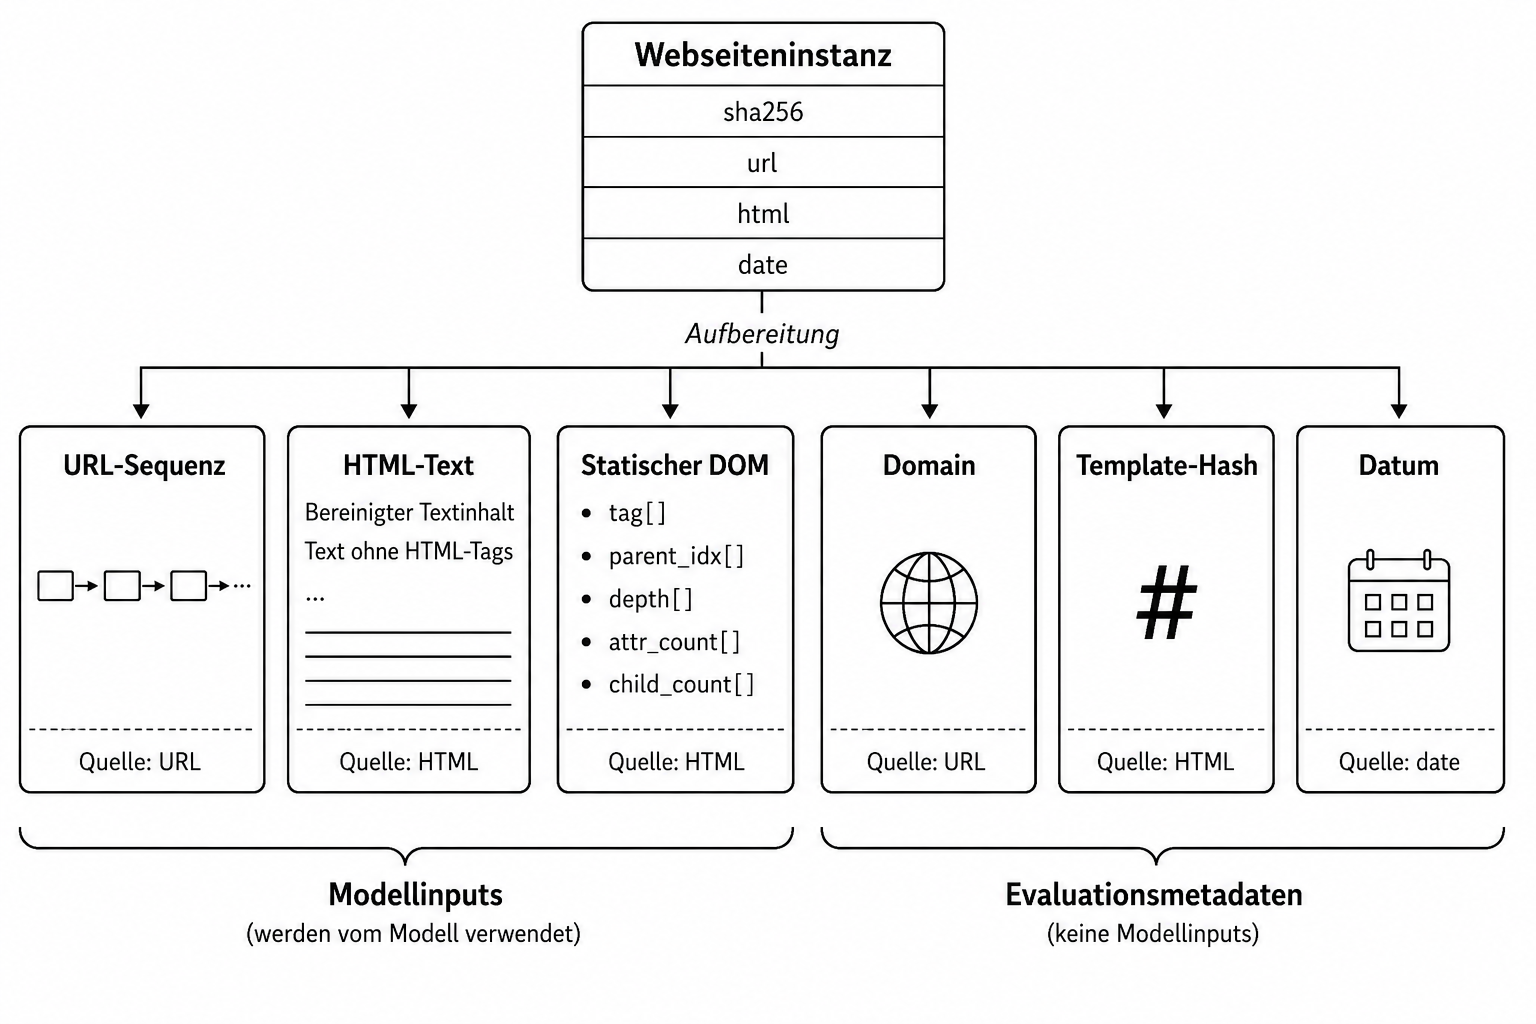
\includegraphics[width=0.85\linewidth]{Praefix/Image/InformationDia.png}
    \caption{Ableitung der Informationsmodalitäten und Evaluationsmetadaten aus einer Webseiteninstanz}
    \label{fig:datenaufbereitung}
{\footnotesize Eigene Darstellung; KI-unterstützt.}
\end{figure}

Aus jeder Webseiteninstanz werden drei Modellinputs und drei Evaluationsmetadaten abgeleitet.
Die URL bleibt als sequenzielle Eingabe erhalten. Aus dem gespeicherten HTML werden ein
bereinigter HTML-Text und ein statischer DOM erzeugt. Für den Text werden Kommentare sowie
Script-, Style-, Noscript- und Template-Bereiche entfernt, anschließend HTML-Tags entfernt,
HTML-Zeichenreferenzen aufgelöst und Whitespace normalisiert. Für den DOM wird das
HTML-Dokument als Baum geparst; pro Knoten werden Tagname, Elternindex, Tiefe,
Attributanzahl und Anzahl direkter Kindknoten gespeichert. Es handelt sich um einen aus dem
gespeicherten HTML rekonstruierten statischen DOM und nicht um einen browserseitig
gerenderten Laufzeit-DOM.
Domain, Template-Hash und Datum werden getrennt davon ausschließlich für die spätere
Evaluation aufbewahrt. Die Domain wird aus der URL bestimmt; der Template-Hash entsteht aus
der normalisierten Folge öffnender und schließender HTML-Tags. Diese drei Größen gehen nicht
als Modellmerkmale in die Klassifikation ein. Abbildung~\ref{fig:datenaufbereitung} fasst die
Trennung von Modellinputs und Evaluationsmetadaten zusammen.

\section{Repräsentations- und Versuchsdesign}

\subsection{Task-adaptive Repräsentationen R0, RU, RT und RUT}

Zur isolierten Untersuchung der task-adaptiven Anpassung wird ein faktorielles
$2\times2$-Design für URL und HTML-Text verwendet. Für jede Modalität stehen der bereits
allgemein selbstüberwacht vortrainierte Basisencoder und eine mittels Masked Language Modeling
auf den ungelabelten Webseitendaten weitertrainierte Variante zur Verfügung. R0 ist damit
keine ``No-SSL''-Bedingung, sondern der nicht zusätzlich task-adaptiv angepasste Ausgangspunkt.
R0 kombiniert BERT Base und RoBERTa Base, RU ausschließlich den angepassten URL-Encoder,
RT ausschließlich den angepassten HTML-Text-Encoder und RUT beide angepassten Encoder.
BERT und RoBERTa bilden festgelegte Ausgangsmodelle ihrer jeweiligen Modalität; untersucht
wird nicht ihre gegenseitige Überlegenheit, sondern der zusätzliche Adaptationsschritt.

Für die Downstream-Analyse werden URL und HTML-Text getrennt encodiert und die Hidden
States unter Berücksichtigung der Attention Mask jeweils zu einer mittleren
Sequenzrepräsentation aggregiert. Die beiden 768-dimensionalen Vektoren werden zu einer für
alle vier Varianten identischen 1.536-dimensionalen Darstellung konkateniert. DOM-Verarbeitung
und multimodale Fusion bleiben in diesem Versuchsblock unberücksichtigt.

\begin{figure}[H]
\centering
\small
\setlength{\tabcolsep}{3pt}
\renewcommand{\arraystretch}{1.18}
\begin{tabular}{p{0.17\textwidth}|p{0.32\textwidth}|p{0.32\textwidth}}
& \centering\textbf{HTML-Text: Basisencoder} & \centering\arraybackslash\textbf{HTML-Text: TAPT-Encoder} \\
\hline
\centering\textbf{URL:\\Basisencoder}
& \centering \fbox{\parbox[c][1.8cm][c]{0.27\textwidth}{\centering\textbf{R0}\\URL: BERT Base\\Text: RoBERTa Base}}
& \centering\arraybackslash \fbox{\parbox[c][1.8cm][c]{0.27\textwidth}{\centering\textbf{RT}\\URL: BERT Base\\Text: RoBERTa TAPT}} \\
\centering\textbf{URL:\\TAPT-Encoder}
& \centering \fbox{\parbox[c][1.8cm][c]{0.27\textwidth}{\centering\textbf{RU}\\URL: BERT TAPT\\Text: RoBERTa Base}}
& \centering\arraybackslash \fbox{\parbox[c][1.8cm][c]{0.27\textwidth}{\centering\textbf{RUT}\\URL: BERT TAPT\\Text: RoBERTa TAPT}} \\
\end{tabular}
\vspace{0.5em}

Alle Varianten: URL-Repräsentation + HTML-Text-Repräsentation $\rightarrow$
1.536-dimensionale Downstream-Darstellung
\caption{Faktorielles Design der task-adaptiven Repräsentationsvarianten}
\label{fig:tapt_design}
{\footnotesize Eigene Darstellung; KI-unterstützt.}
\end{figure}

\subsection{Downstream-Probes, Labelbudgets und Referenzverfahren}

Zur Bewertung der Repräsentationen werden eine logistische Regression als Linear Probe und ein
kleines Mehrschicht-Perzeptron als nichtlineare Probe eingesetzt. Die Transformer-Encoder
bleiben dabei eingefroren. Die Linear Probe misst die unmittelbare lineare Nutzbarkeit der
Repräsentationen für die Zielklassifikation (vgl. [Chen et al. (2020), PDF-S. 3]). Innerhalb einer
Wiederholung erhalten R0, RU, RT und RUT identische gelabelte Trainingsinstanzen und denselben
Downstream-Versuchsaufbau.

Die Downstream-Supervision wird über sieben verschachtelte Budgets von 2.000 bis 200.000
gelabelten Webseiten variiert. Die vollständigen Lernkurven werden mit fünf gepaarten
Wiederholungen bestimmt; für den zentralen Vergleich RUT gegen R0 bei 20.000 Labels wird auf
zehn Paare erweitert. Die TAPT-Checkpoints werden dabei nicht neu trainiert, sodass N10 die
Variation der Labelauswahl und des Downstream-Trainings bei festen Repräsentationen erfasst.
Die Budgets unter 200.000 enthalten je zur Hälfte beide Klassen und sind innerhalb einer
Wiederholung ineinander verschachtelt. Bei 200.000 wird dagegen der vollständige SSL-Bestand
mit 101.578 benignen und 98.422 Phishing-Instanzen verwendet. Die Auswahl benötigt somit
Klasseninformationen, obwohl diese beim vorgelagerten TAPT nicht eingelesen werden. FF3 nutzt dasselbe Budgetraster für den Vergleich mit R0@200k als interner Referenz sowie einer
mit 200.000 Labels trainierten TF-IDF/XGBoost-Pipeline. Da sich bei letzterer zugleich
Repräsentation und Klassifikator ändern, wird dieser Vergleich nur als verfahrensübergreifende
Referenz interpretiert. Ergänzend wird die Label-Effizienz von R0 und RUT auf dem unabhängig
erhobenen Phishing Website Dataset von Putra (2023) geprüft. Der Datensatz wird anhand des
Erfassungszeitpunkts in einen früheren Trainings- und einen späteren Testbestand getrennt. Auf
dem früheren Bestand werden für beide Repräsentationen identische, verschachtelte Budgets von
200, 500, 1.000 und 2.000 gelabelten Webseiten mit zehn gepaarten Linear-Probes verwendet.
Primärer Endpunkt ist die über die logarithmierten Labelbudgets integrierte
Average-Precision-Lernkurve (AP-AULC).

Für Putra werden 10.391 vollständige Datensätze nach Erfassungszeitpunkt geordnet.
Der Schnitt am empirischen 75-\%-Quantil (7. April 2023, 03:33:03,372 UTC) ergibt
7.793 frühere Instanzen (3.554 benign, 4.239 Phishing) und 2.598 spätere Instanzen
(1.686 benign, 912 Phishing); exakte URL-Überschneidungen zwischen beiden Teilen
wurden nicht gefunden. Verarbeitet werden die URL und das bereitgestellte Textmerkmal,
kein neu gerendertes HTML. Die externen Auswertungen sind nachträgliche Transferanalysen.
In einem zusätzlichen Vergleich werden beide Quell-RUT-Encoder über eine MLM-Epoche
auf dem ungelabelten frühen Putra-Pool angepasst (E1); E0 behält die Quell-RUT-Encoder bei.
Beide verwenden dieselben zehn Labelauswahlen und das unveränderte externe Testset.
Der zusätzliche MLM-Schritt verwendet 15\,\% Maskierung, Lernrate $5\cdot10^{-5}$,
Weight Decay 0,01 und 6\,\% Warmup. Das spätere Putra-Testset wird hierfür nicht verwendet.

Ein früherer explorativer Versuchsblock untersucht ergänzend kontrastive Repräsentationen.
R2C und R3C kombinieren modalitätsinterne Ansichten mit URL--HTML-Positivpaaren, während
CSAME nur modalitätsinterne Paare nutzt; Domain- und Template-Identitäten werden aus den
Negativmengen ausgeschlossen. Da dieser Block nicht unter dem finalen R0/RU/RT/RUT-Protokoll
wiederholt wurde, erfolgt ausschließlich eine deskriptive Einordnung anhand der
zugehörigen eigenen Ergebnisartefakte.

\section{Evaluations- und Statistikdesign}

\subsection{Kalibration und Evaluationsbedingungen}

Für die schwellenwertabhängige FINAL-Evaluation wird CAL mit 50.000 ausschließlich legitimen
Webseiten verwendet. Für jede zu bewertende Modell- und Wiederholungskonfiguration wird auf
diesen benignen Instanzen ein Schwellenwert für eine Ziel-False-Positive-Rate von 0,5\,\%
bestimmt. Dieser Wert ist ein festgelegter restriktiver Betriebspunkt der vorliegenden
Untersuchung und kein allgemeiner Standard für Phishing-Erkennungssysteme. Der auf CAL
bestimmte Schwellenwert wird unverändert auf den vollständigen Finalbestand und die daraus
gebildeten Bedingungen übertragen.

\begin{table}[htbp]
\centering
\small
\setlength{\tabcolsep}{4pt}
\renewcommand{\arraystretch}{1.12}
\caption{Evaluationsbedingungen der abschließenden Generalisierungsbewertung.}
\label{tab:testszenarien}
\begin{tabular}{p{0.24\textwidth}p{0.55\textwidth}r}
\hline
\textbf{Bedingung} & \textbf{Operationalisierung} & \textbf{Umfang} \\
\hline
Official Test & Vollständiger offizieller Testbestand & 168.060 \\
Domain-OOD & Domain zuvor nicht in den entwicklungszugänglichen Datenrollen beobachtet & 115.917 \\
Template-OOD & Template-Hash zuvor nicht in den entwicklungszugänglichen Datenrollen beobachtet & 161.223 \\
Domain+Template-OOD & Weder Domain noch Template-Hash zuvor beobachtet & 110.095 \\
Late Test Q4 & Erfassungsdatum ab dem 75-\%-Quantil des Finalbestands & 46.784 \\
\hline
\end{tabular}
\end{table}

Die Zeitbedingung beginnt am 28.10.2025, dem 75-\%-Quantil der Erfassungsdaten.
Wegen gleicher Datumswerte an der Grenze umfasst sie 46.784 Fälle und damit mehr als
genau ein Viertel des Finalbestands.

Zur zusätzlichen Absicherung der Szenariodefinition wurde ein metadatenbasierter
Integritätsaudit durchgeführt. Die exakten Domain- und \nolinkurl{template_hash}-Identitäten der
FINAL-Szenarien wurden hierzu mit SUP, DEV, CAL und dem 200.000 Instanzen umfassenden
SSL/TAPT-Pool abgeglichen. Für alle prüfbaren Domain-OOD- und Template-OOD-Instanzen
ergab sich keine einzige exakte Überschneidung; dies gilt ebenso für das kombinierte
Domain+Template-OOD-Szenario. Für die vorhandenen Identitätswerte weist der Audit somit keine Exposition gegenüber den
geprüften Lernrollen nach; dies bezieht sich auf exakte Identitäten und den archivierten Freeze. Für 1,34\,\% der Domain-OOD-Instanzen beziehungsweise 1,38\,\% im
kombinierten Szenario lag kein auswertbarer Domainwert vor; semantische Ähnlichkeiten oder
Near-Duplicates werden in dieser Arbeit nicht geprüft.

\subsection{Statistische Entscheidungsregeln}

Bei gepaarten Repräsentations- und Architekturvergleichen bildet die jeweilige
Trainingsreplikation die statistische Einheit. Als Effektgröße wird die mittlere Differenz der TPR
in Prozentpunkten berichtet. Für mittlere Paardifferenzen wird das zweiseitige t-Intervall
$\bar d\pm t_{0{,}975;n-1}s_d/\sqrt n$ verwendet; es beschreibt die
Downstream-Variation bei festen Vortrainingszuständen und fester Testpopulation.
Die t-Intervalle setzen unabhängige, näherungsweise normalverteilte Paardifferenzen voraus;
die Sign-Flip-Tests benötigen unter der jeweiligen Nullhypothese Vorzeichensymmetrie.
Die vollständige Enumeration allein macht einen Test nicht voraussetzungsfrei.
Ergänzend werden die Anzahl der
Replikationen mit positiver beziehungsweise negativer Differenz angegeben. Für gepaarte
Vergleiche wird der exakte Sign-Flip-Permutationstest verwendet (vgl. [Holt und Sullivan (2023), S. 787--788]). Mehrere gemeinsam geprüfte Hypothesen werden mit der Holm-Prozedur für
multiples Testen korrigiert (vgl. [Holm (1979), S. 66--67]). Der N10-Vergleich von RUT20k und R020k verwendet \nolinkurl{OFFICIAL_TEST} als primären
Endpunkt. Die vier zusätzlichen domain-, template- und zeitbezogenen Bedingungen bilden eine
gemeinsame sekundäre Testfamilie; ihre vier p-Werte werden innerhalb dieses Vergleichs nach
Holm korrigiert.

Für FF3 wird eine Nichtunterlegenheitsmarge von einem Prozentpunkt TPR festgelegt. Gegen
R0@200k wird für jedes Budget und jede Evaluationsbedingung ein exakter einseitiger
Sign-Flip-Test auf die um diese Marge verschobene gepaarte Differenz berechnet. Ein Budget
gilt nur dann als ausreichend, wenn die Nichtunterlegenheit in allen fünf Bedingungen
gleichzeitig erreicht wird. Der gemeinsame p-Wert ist das Maximum der fünf
Komponenten-p-Werte (Intersection-Union-Prinzip). Anschließend werden die sieben Budgetentscheidungen mit der
Holm-Prozedur korrigiert. Die Marge von einem Prozentpunkt dient als Entscheidungsschwelle
dieser Untersuchung und stellt keine fachlich oder betrieblich validierte Servicegrenze dar. Für den Vergleich von RUT+Linear mit TF-IDF/XGBoost@200k besteht keine natürliche
Paarung der zehn Modellläufe. Deshalb werden die Beobachtungen nicht nachträglich einander
zugeordnet. Dieser nachträgliche Welch-Vergleich wird als ergänzende, verfahrensübergreifende
Evidenz interpretiert. Stattdessen wird für jede Evaluationsbedingung ein einseitiger
Welch-Nichtunterlegenheitstest mit derselben Marge berechnet. 

Auch hier muss die
Nichtunterlegenheit in allen fünf Bedingungen erreicht werden; anschließend werden die sieben
Budgetentscheidungen nach Holm korrigiert. Zusätzlich wird deskriptiv ausgewiesen, ab welchem Budget die mittlere TPR von RUT in allen
fünf Bedingungen mindestens der XGBoost-TPR entspricht und die mittlere FPR gleichzeitig
nicht höher liegt. Diese zusätzliche Auswertung beschreibt ausschließlich die beobachteten
Mittelwerte und stellt keinen Signifikanztest dar.

Da die Nichtunterlegenheitsmarge von einem Prozentpunkt für diese Untersuchung festgelegt
wurde, wird nach Abschluss der primären FF3-Auswertung ergänzend geprüft, wie stark die
ermittelte Budgetstufe von dieser Festlegung abhängt. Hierzu wird dasselbe N10-Protokoll
zusätzlich mit TPR-Margen von 0,0, 0,5 und 2,0 Prozentpunkten ausgewertet. Gegen R0@200k
bleiben der gepaarte einseitige Sign-Flip-Test, die gleichzeitige Bedingung über alle fünf
Evaluationsbedingungen und die Holm-Korrektur über sieben Budgets unverändert. Für
TF-IDF/XGBoost@200k wird analog mit den einseitigen Welch-Tests verfahren. Bei einer
Marge von 0,0 Prozentpunkten wird kein TPR-Nachteil zugelassen; die Entscheidung verlangt
damit einen über alle fünf Bedingungen positiven Unterschied im verwendeten Testprotokoll. Die Sensitivitätsanalyse wurde nach der primären 1-pp-Auswertung ergänzt. Sie dient
ausschließlich dazu, die Stabilität der resultierenden Budgetstufe gegenüber alternativen Margen
zu prüfen. Die 1-pp-Marge bleibt die vorab verwendete Hauptentscheidung und wird durch die
ergänzende Auswertung nicht nachträglich ersetzt.

\section{Konzeption des prototypischen Klassifikationssystems}

\subsection{Zielbild und Gesamtarchitektur}



Aufbauend auf der Repräsentationsanalyse wird ein mehrzweigiges prototypisches
Klassifikationssystem konzipiert. Die DUAL-Variante verarbeitet URL und HTML-Text in
getrennten Transformerzweigen. Die TRI-Variante ergänzt zusätzlich die strukturelle
DOM-Repräsentation. Die Ausgaben der aktiven Modalitäten werden jeweils in einen gemeinsamen
256-dimensionalen Raum projiziert und L2-normalisiert. Eine lernbare Gating-Komponente
bestimmt instanzabhängige Modalitätsgewichte; daraus wird eine gewichtete
Fusionsrepräsentation gebildet. Die Verwendung lernbarer, über Softmax normalisierter
Modalitätsgewichte entspricht dem Prinzip einer gewichteten multimodalen Fusion
(vgl. [Zhou et al. (2019), PDF-S. 2]). 
Für die abschließende Klassifikation werden die einzelnen
Modalitätsrepräsentationen gemeinsam mit der Fusionsrepräsentation verwendet.
Modalitätsspezifische Auxiliary Heads erzeugen zusätzliche Hilfsscores, ohne die
Gating-Gewichte zu ersetzen. Der URL-Hilfsscore bildet zugleich die Grundlage der
URL-first-Kaskade. Die Gesamtarchitektur und die Rollen von DUAL, TRI, Auxiliary Heads,
Gating und Main Head sind in Abbildung~\ref{fig:systemkonzeption} dargestellt. Die technische
Parametrisierung der Encoderfreigabe, DOM-GCN-, Gating- und Head-Komponenten wird erst
in Kapitel 5 spezifiziert. Die Architektur trennt damit drei Ebenen: die Repräsentationsbildung innerhalb der
Modalitätszweige, deren gemeinsame Fusion und die nachgelagerte Klassifikation. Ob jede
zusätzliche Systemkomponente gegenüber einer einfacheren Vorstufe einen eigenen Beitrag
liefert, wird nicht aus dem Endmodell abgeleitet, sondern in einer gesonderten sequenziellen
Ablation geprüft.

\begin{figure}[H]
    \centering
    \makebox[\textwidth][c]{%
        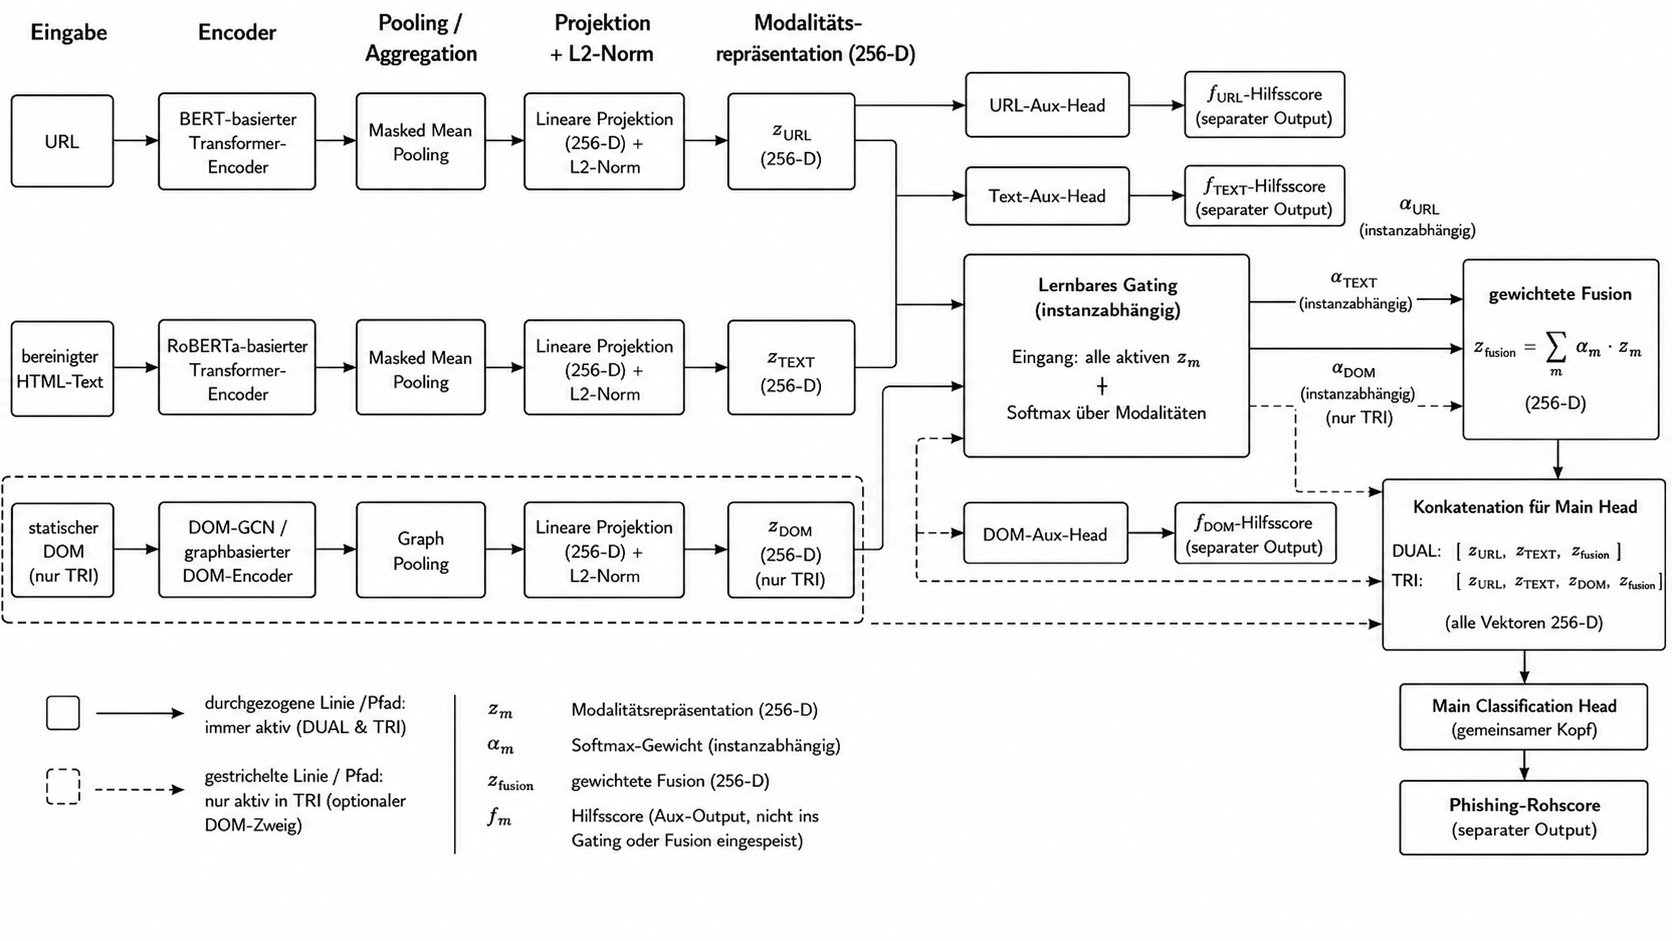
\includegraphics[width=1.0\textwidth]{Praefix/Image/Systemkonzeption.png}%
    }
    \caption{Gesamtarchitektur des prototypischen Klassifikationssystems}
    \label{fig:systemkonzeption}
    \vspace{0.2em}
{\footnotesize Eigene Darstellung; KI-unterstützt.}
\end{figure}

\subsection{Sequenzielle Komponentenablation}

Zur kontrollierten FF4-Komponentenprüfung wird die RUT-Repräsentationsbasis festgehalten und
vier verschachtelte Systemvarianten werden verglichen:
\[
\begin{aligned}
P_0&=\text{URL}, &
P_1&=\text{URL+Text, Equal},\\
P_2&=\text{URL+Text+DOM, Equal}, &
P_3&=\text{URL+Text+DOM, Gated}.
\end{aligned}
\]

Damit quantifiziert $P_1-P_0$ den zusätzlichen Textbeitrag, $P_2-P_1$ den zusätzlichen
DOM-Beitrag und $P_3-P_2$ den Beitrag der lernbaren Gating-Fusion. Die vier Varianten
werden mit zehn gepaarten Replikationen auf derselben balancierten Stichprobe aus
20.000 Labels trainiert. Die initialen RUT-URL- und Textcheckpoints sowie der DOM-SSL-Encoder bleiben
identisch; die freigegebenen Modellparameter werden überwacht trainiert. Für alle Varianten werden eine Epoche und Batchgröße acht verwendet. Die Komponentenablation verwendet ausschließlich Development-Daten. Der Schwellenwert wird
auf den benignen Beispielen der Teilmenge \nolinkurl{ENG_TUNE} bei einer Ziel-FPR von
0,5\,\% bestimmt. Primärer Endpunkt der Komponentenablation ist die TPR auf der von
\nolinkurl{ENG_TUNE} getrennten Teilmenge \nolinkurl{ENG_META}. CAL und FINAL werden für
diese Analyse nicht verwendet. Für die drei benachbarten N10-Vergleiche werden exakte
zweiseitige Sign-Flip-Tests berechnet und gemeinsam nach Holm korrigiert.

\subsection{URL-first-Kaskade und Frontend-Vergleich}

\begin{figure}[H]
    \centering
    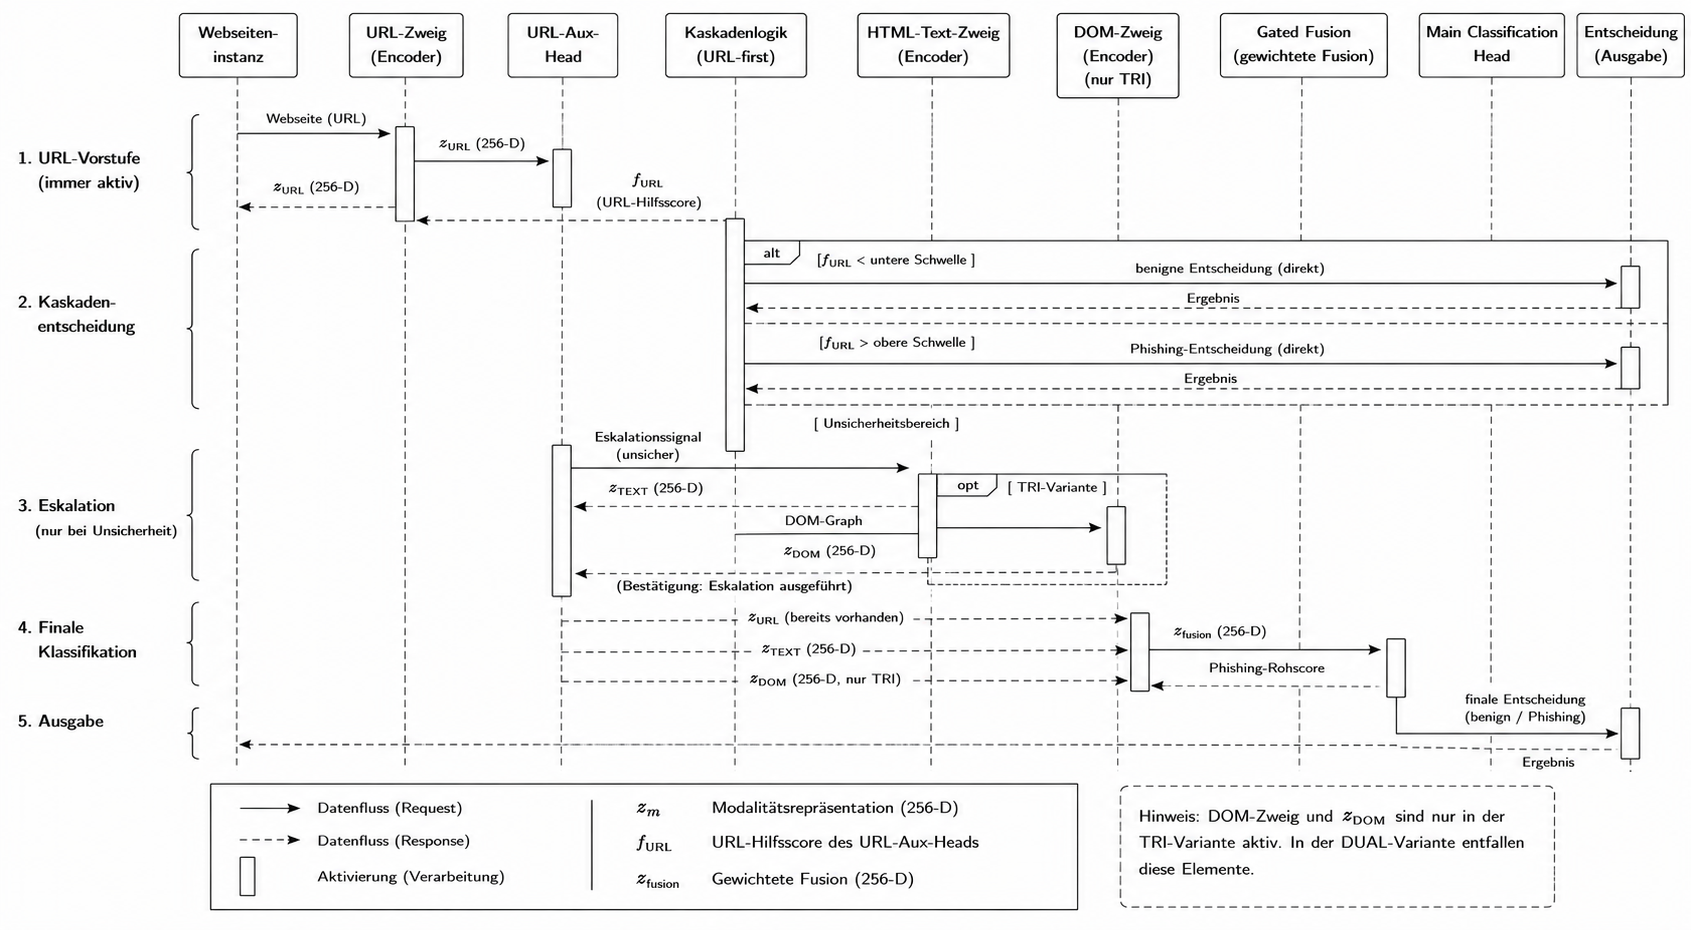
\includegraphics[width=1\linewidth]{Praefix/Image/URLKaskade.png}
    \caption{Sequenzdiagramm der bedingten Verarbeitung in der URL-first-Kaskade}
    \label{fig:urlkaskade}
{\footnotesize Eigene Darstellung; KI-unterstützt.}
\end{figure}

Die URL-first-Kaskade führt zunächst ausschließlich den URL-Zweig aus und erzeugt über den
URL-Auxiliary-Head den Score $f_{\mathrm{URL}}$. Eine untere und eine obere, auf
Development-Daten bestimmte Schwelle begrenzen einen Unsicherheitsbereich. Liegt der Score
außerhalb dieses Bereichs, wird die Klassifikation bereits nach dem URL-Pfad abgeschlossen.
Nur die dazwischenliegenden Fälle durchlaufen zusätzlich den vollständigen multimodalen Pfad.
Dieses Vorgehen entspricht dem Grundprinzip kaskadierter Klassifikatoren
(vgl. [Viola und Jones (2004), S. 144--145]). Bei einer Eskalation wird die bereits berechnete URL-Repräsentation wiederverwendet und um
HTML-Text sowie in der TRI-Variante um den DOM ergänzt. Die aktiven Repräsentationen
durchlaufen anschließend dieselbe Fusion und denselben Klassifikationskopf wie im Vollsystem.
Abbildung~\ref{fig:urlkaskade} zeigt den Ablauf und verdeutlicht, dass der DOM-Zweig nur für
eskalierte TRI-Fälle ausgeführt wird. Zusätzlich wird untersucht, ob die verwendete URL-Repräsentation den Anteil der Eskalationen
beeinflusst. TRI-Fallback, Labelbudget und grundsätzliche Routinglogik bleiben hierfür
unverändert; variiert wird ausschließlich zwischen der Basis- und der task-adaptierten
URL-Repräsentation. Die Routingparameter werden auf Development-Daten für zulässige
TPR-Abweichungen von 0,25, 0,5, 1,0 und 2,0 Prozentpunkten gegenüber dem Vollsystem
bestimmt. Die primär betrachtete Toleranz beträgt einen Prozentpunkt. Als zentrale
Ressourcenkennzahl wird die Eskalationsrate berichtet, also der Anteil der Webseiten, für die
der vollständige multimodale Pfad ausgeführt wird. Verglichen wird damit der erforderliche
Verarbeitungsumfang unter derselben vorgegebenen TPR-Toleranz.

\section{Freeze, Reproduzierbarkeit und Grenzen des Untersuchungsdesigns}

Die ursprüngliche Repräsentations- und Systementwicklung erfolgt auf den vorgesehenen
Development-Daten; vor dem Zugriff auf CAL und FINAL wird für den finalen Integrationslauf
ein Architecture-Freeze gespeichert. CAL wird danach ausschließlich zur Schwellenwertbestimmung
verwendet, während FINAL und die daraus gebildeten Teilmengen ausschließlich der abschließenden
Leistungsbewertung dienen. Datenrollen, Modellzustände, Konfigurationen, Seeds und
Auswertungsartefakte werden gespeichert sowie die Disjunktheit der Datenrollen, die erwarteten
Instanzzahlen und die Vollständigkeit der Ergebnisartefakte automatisiert geprüft.

Mehrere ergänzende Analysen wurden erst nach Vorliegen früherer Ergebnisse durchgeführt.
Der Vergleich mit TF-IDF/XGBoost wurde nach den ersten RUT/R0-Ergebnissen um das
vollständige Budgetraster von 2.000 bis 200.000 Labels erweitert; sämtliche sieben
Budgetstufen werden berichtet und der Analyseplan wurde vor der Ausführung gespeichert.
Auch die sequenzielle FF4-Komponentenablation wurde erst nach Festlegung der finalen
Architektur ergänzt. Varianten, neue Seeds, die drei Komponentenvergleiche und die
Schwellenlogik wurden vor ihrer Durchführung festgelegt, während CAL und FINAL weiterhin
ausgeschlossen blieben. Die Komponentenablation dient damit der nachträglichen Prüfung der
bereits festgelegten Systembestandteile und nicht der erneuten Auswahl der finalen Architektur. Die Sensitivitätsanalyse der FF3-Marge wurde nach Abschluss der primären 1-pp-Auswertung
ergänzt und wendet ohne erneutes Modelltraining dieselben statistischen Entscheidungsregeln
auf alternative Margen von 0,0, 0,5 und 2,0 Prozentpunkten an. Sie prüft ausschließlich, ob
sich die kleinste ausreichende Budgetstufe bei alternativen Festlegungen verändert. Die
Wiederholungen variieren die Labelauswahl und das Downstream-Training bei unveränderten
Repräsentations- beziehungsweise Pretraining-Checkpoints und erfassen daher nicht die Varianz
vollständig neu ausgeführter selbstüberwachter Vortrainingsläufe. Aussagen zur reduzierten
Labelmenge beziehen sich ausschließlich auf die gelabelte Downstream-Supervision.


Die betriebliche Szenarioanalyse wird nach Abschluss der Modellauswertung ergänzt. Sie
verwendet die eingefrorenen FINAL-Konfusionsmatrizen und klassenspezifischen Routinganteile,
ohne Schwellen neu auszuwählen. Referenzvolumen und Phishinganteile sind ausdrücklich
angenommene Größen. Die Umrechnung setzt unverändertes Fehler- und Routingverhalten
innerhalb beider Klassen voraus; ihre Werte sind bedingte Erwartungswerte ohne zusätzliche
Unsicherheitsintervalle. Der gemessene In-Memory-Durchsatz bleibt eine separate technische
Referenz. Ein betrieblicher Pilot oder ein neuer Verteilungstest wird dadurch nicht ersetzt.

\lstset{
  basicstyle=\ttfamily\small,
  numbers=left,
  numberstyle=\tiny,
  stepnumber=2,
  numbersep=6pt,
  frame=single,
  framerule=0.3pt,
  breaklines=true,
  breakatwhitespace=false,
  breakindent=1.0em,
  columns=fullflexible,
  keepspaces=true,
  showstringspaces=false,
  xleftmargin=2.4em,
  xrightmargin=0.5em,
  aboveskip=0.30\baselineskip,
  belowskip=0.30\baselineskip,
  captionpos=b
}


\chapter{Implementierung}

\section{Entwicklungs- und Ausführungsumgebung}

Die experimentelle Pipeline wurde Python-basiert in einer GPU-gestützten
Kaggle-Notebook-Umgebung umgesetzt. Für Training und Inferenz der neuronalen
Modellkomponenten wird PyTorch verwendet, während die transformerbasierten Encoder und
Tokenizer über die Transformers-Bibliothek eingebunden werden. Ergänzend kommen NumPy,
pandas und PyArrow für die Datenverarbeitung sowie scikit-learn und SciPy für
Downstream-Modelle und statistische Auswertungen zum Einsatz. Das statische HTML- und
DOM-Parsing der vorgelagerten Data-Freeze-Pipeline basiert auf lxml.

Die rechenintensiven Verarbeitungsschritte werden CUDA-beschleunigt ausgeführt. Die finale
Integrationspipeline prüft hierzu beim Start die Verfügbarkeit einer GPU und verwendet eine
NVIDIA-Tesla-T4-Umgebung als Zielkonfiguration. Für Trainings- und Inferenzoperationen ist
darüber hinaus Mixed Precision aktiviert; die entsprechenden Berechnungen werden über
\texttt{torch.autocast} mit \texttt{float16} ausgeführt. Speicherintensive
Verarbeitungsblöcke enthalten zusätzliche CUDA-Speicherbereinigungen. Für mehrere Trainings-
und Scoring-Schritte sind zudem abgestufte Batchgrößen implementiert, sodass ein
Verarbeitungsschritt bei einem \texttt{OutOfMemoryError} mit einer kleineren
Batchkonfiguration erneut ausgeführt werden kann. Die jeweils verwendeten Batchgrößen werden
bei den zugehörigen Modellkomponenten konkretisiert.

Für die reproduzierbare Durchführung der wiederholten Experimente werden die verwendeten
Zufallsquellen zentral initialisiert. Der Gesamtlauf verwendet den Master-Seed 20260817; die
einzelnen Versuchsblöcke greifen ergänzend auf festgelegte Modell- und Ranking-Seeds zurück.
Die Initialisierung umfasst Python, NumPy und PyTorch einschließlich der CUDA-Zufallsquellen.

Die während der Ausführung erzeugten Modellzustände, vorberechneten Repräsentationen,
Vorhersagescores sowie Ergebnis- und Auditinformationen werden getrennt als Artefakte
gespeichert. Die darauf aufbauenden Completion-, Freeze- und Reproduzierbarkeitsmechanismen
werden in Abschnitt 5.6 beschrieben.

\section{Implementierung der Datenverarbeitung}

Die Datenverarbeitung bildet den gemeinsamen Ausgangspunkt sämtlicher nachfolgenden
Versuchsblöcke. Der PhreshPhish-Datensatz wird zunächst in einem festen Data Freeze geprüft,
aufbereitet und in die in Abschnitt 4.2.1 definierten Rollen SUP, DEV, CAL und SSL überführt.
Der offizielle Testbestand bleibt davon getrennt und wird erst in den späteren
Evaluationsschritten als FINAL verwendet. Während des Data Freeze werden unter anderem die
erwarteten Rollenstärken, doppelte SHA-256-Identifikatoren und exakte Überschneidungen
zwischen Trainings- und Testbestand programmatisch geprüft.

Die Rollenbildung erfolgt deterministisch über die SHA-256-Identifikation der einzelnen
Webseiten. Hierzu wird der jeweilige Identifikator gemeinsam mit einem festen,
rollenspezifischen Zusatzstring erneut gehasht. Im Code wird dieser Zusatz als \texttt{salt}
bezeichnet. Dadurch entstehen für die unterschiedlichen Auswahlstufen getrennte, bei erneuter
Ausführung jedoch identische Rangfolgen. Listing~\ref{lst:stable_rank} im Anhang zeigt die hierfür
verwendete Funktion.



SUP und DEV werden auf dieser Grundlage jeweils klassenweise gebildet. CAL wird
anschließend ausschließlich aus noch nicht zugeordneten benignen Instanzen bestimmt, bevor
der SSL-Pool aus dem verbleibenden Bestand abgeleitet wird. Die Implementierung prüft
abschließend die vorgesehenen Größen von 4.000 SUP-, 20.000 DEV-, 50.000 CAL- und
200.000 SSL-Instanzen. Die deterministische Materialisierung setzt damit die in
Abschnitt 4.2.1 konzipierte Trennung der Datenrollen technisch um. Parallel zur Rollenbildung
werden die in Abschnitt 2.1.2 unterschiedenen Informationsperspektiven für die nachfolgenden
Modellzweige aufbereitet.

Für den textuellen HTML-Zweig werden zunächst Kommentare sowie \texttt{script}-,
\texttt{style}-, \texttt{noscript}- und \texttt{template}-Bereiche entfernt.
Anschließend werden die verbleibenden Tags entfernt, HTML-Zeichenreferenzen aufgelöst und
Whitespace normalisiert. Aus den normalisierten HTML-Tags wird zusätzlich eine strukturelle
Sequenz gebildet. Diese dient unter anderem zur Ableitung des \nolinkurl{template_hash}, der
später für die Template-basierten OOD-Szenarien benötigt wird.
Listing~\ref{lst:process_row} im Anhang fasst die für Text-, Template- und DOM-Ableitung maßgeblichen
Verarbeitungsschritte zusammen.



Der Ausschnitt zeigt nur die für die beschriebenen Ableitungen relevanten Teile der Funktion;
die vollständige Implementierung verbleibt in den digitalen Artefakten. Die DOM-Struktur wird
aus dem gespeicherten HTML statisch rekonstruiert. Für jeden berücksichtigten Knoten werden
Tagname, Elternindex, Tiefe, Attributanzahl und Anzahl direkter Kindknoten gespeichert. Damit
bleibt die in Abschnitt 2.2.2 beschriebene graphbasierte Sicht auf die
Eltern-Kind-Beziehungen des HTML-Dokuments für den späteren DOM-Zweig erhalten. Im Data
Freeze werden maximal 4.096 DOM-Knoten pro Webseite materialisiert; die engere
Eingabegrenze des Deep-Modells wird erst in Abschnitt 5.4 angewendet.

Eine zentrale technische Trennung betrifft den SSL-Pool. Entsprechend dem in Abschnitt 2.3
beschriebenen Prinzip des selbstüberwachten Lernens werden dessen physische Parquet-Dateien
ohne Downstream-Label gespeichert. Die Spalte \texttt{label} wird bereits während der
Rollenmaterialisierung explizit entfernt, wie Listing~\ref{lst:remove_label} im Anhang zeigt.



Die finale Pipeline kontrolliert zusätzlich über das Parquet-Schema, dass die physischen
SSL-Dateien weiterhin keine Labelspalte enthalten. Die Klasseninformationen verbleiben
getrennt in einem privaten Rollenmanifest und werden erst für die späteren überwachten
Labelbudgetexperimente über die SHA-256-Identifikation wieder zugeordnet. Die TAPT-Verfahren
arbeiten dagegen ausschließlich auf den physisch label-freien Webseiteninformationen. Damit
wird die experimentelle Trennung zwischen verfügbarem ungelabeltem Trainingsmaterial und
verfügbarer überwachter Trainingsinformation nicht nur konzeptionell, sondern auch in der
Datenpipeline umgesetzt.

\section{Implementierung der Self-Supervised Repräsentationen}

Die in Abschnitt 2.3 eingeführte selbstüberwachte Repräsentationsanpassung wird getrennt für
die URL- und die HTML-Text-Modalität umgesetzt. Als Ausgangspunkt dienen mit
\texttt{bert-base-uncased} beziehungsweise \texttt{roberta-base} bereits vortrainierte
Transformerencoder. Beide Modelle werden mittels Masked Language Modeling auf den
200.000 physisch label-freien Instanzen des SSL-Pools weitertrainiert. Damit wird das in
Abschnitt 2.3.3 beschriebene Task-Adaptive Pretraining auf dem aufgabenspezifischen
Webseiten-Trainingspool umgesetzt, ohne hierfür das Downstream-Label Phishing
beziehungsweise Benign zu verwenden.

Für die Modalitäten gelten unterschiedliche Kontextgrenzen: Der URL-Zweig verarbeitet
maximal 128 BERT-Token einschließlich Spezialtoken. Längere Eingaben werden abgeschnitten.
Eine vollständige Abdeckung des URL-Bestands durch diese Grenze ist damit nicht belegt.

Für den HTML-Text wird dagegen ein festes Kontextbudget von 256 Tokens verwendet. Die
HTML-Dokumente besitzen gegenüber URLs wesentlich umfangreichere und stärker variierende
Sequenzen. Die Begrenzung dient daher insbesondere dazu, Speicherbedarf und Rechenaufwand
des transformerbasierten Trainings kontrollierbar zu halten. Sie ist nicht als Annahme zu
verstehen, dass innerhalb von 256 Tokens der vollständige HTML-Inhalt einer Webseite erfasst
wird. Von dieser Transformergrenze ist die vorgelagerte Datenaufbereitung zu unterscheiden:
Im Data Freeze wird der bereinigte HTML-Text zunächst mit bis zu 50.000 Zeichen
materialisiert; die Begrenzung auf 256 Tokens erfolgt erst bei der Eingabe in den Textencoder.

Für beide Modalitäten wird das TAPT über eine Epoche durchgeführt. Da die Encoder dabei
nicht neu initialisiert, sondern bereits vortrainierte BERT- beziehungsweise RoBERTa-Modelle
zusätzlich an den Webseiten-Trainingspool angepasst werden, bildet eine Epoche ein bewusst
begrenztes Adaptationsbudget für den zusätzlichen SSL-Schritt. Beide Zweige durchlaufen damit
den jeweils 200.000 Instanzen umfassenden SSL-Bestand einmal vollständig. Die Festlegung ist
als einheitliche experimentelle Vorgabe und nicht als Aussage über ein global optimales
Trainingsbudget zu verstehen.

Für das URL-TAPT werden 15\,\% MLM-Maskierung, AdamW, eine Lernrate von
$5\cdot 10^{-5}$, Weight Decay 0,01 und 6\,\% Warmup verwendet.
Listing~\ref{lst:url_tapt} im Anhang zeigt die dafür maßgebliche Trainingskonfiguration.



Der TAPT-Pfad liest ausschließlich URLs aus dem physischen SSL-Pool; als Batch-Fallback
sind 16 und 8 hinterlegt. Für den HTML-Text-Zweig wird derselbe MLM-Mechanismus mit
15\,\% Maskierung, $5\cdot 10^{-5}$ Lernrate, Weight Decay 0,01 und 6\,\% Warmup
verwendet. Aufgrund der längeren Textsequenzen sind dort Batch-Fallbacks von 16, 8 und 4
vorgesehen. Der vollständige Trainingscode beider Zweige ist in den digitalen Artefakten
enthalten.

Die getrennte Anpassung beider Modalitäten bildet die technische Grundlage des in
Abschnitt 4.3.1 beschriebenen $2\times2$-Versuchsdesigns. Hierzu werden jeweils Basis- und
TAPT-Encoder so kombiniert, dass der Anpassungseffekt beider Modalitäten getrennt variiert
werden kann. R0 verwendet für URL und HTML-Text die unveränderten Ausgangsmodelle, RU
ausschließlich den angepassten URL-Encoder, RT ausschließlich den angepassten Textencoder
und RUT die TAPT-Varianten beider Zweige. Die verwendeten Encoderquellen werden für jede
Variante in den Audit-Artefakten gespeichert.

Damit bleibt die nachgelagerte Repräsentationsbildung zwischen den vier Bedingungen
strukturell identisch; variiert wird ausschließlich die Herkunft des URL- beziehungsweise
Textencoders. Auf diese Weise kann der zusätzliche Nutzen der task-adaptiven Anpassung
zunächst unabhängig von den späteren Architekturkomponenten wie DOM-Zweig und
multimodaler Fusion untersucht werden.

Für die kontrollierten Downstream-Probes werden aus den Hidden States der jeweiligen
Transformer feste Repräsentationsvektoren erzeugt. Hierzu wird ein
attention-mask-basiertes Mean Pooling verwendet, sodass Padding-Token nicht in die
Mittelwertbildung eingehen. Die Summe der gültigen Hidden States wird dabei durch die Anzahl
der über die Attention Mask markierten Token geteilt.

Die URL- und Textrepräsentationen werden getrennt extrahiert und als
\texttt{float32}-Embeddings zwischengespeichert. Die beiden 768-dimensionalen Vektoren werden
anschließend zu der in Abschnitt 4.3.1 definierten 1.536-dimensionalen Gesamtrepräsentation
konkateniert. Im Probe-Pfad erfolgt danach keine gemeinsame Weiteroptimierung der
Transformerencoder mit dem Klassifikator. Auf den festen Repräsentationen werden stattdessen
eine logistische Regression als Linear Probe sowie ein kleines MLP trainiert. Damit wird der
Repräsentationseffekt von Veränderungen der späteren End-to-End-Architektur getrennt.

Die Probe-Experimente werden für die sieben in Abschnitt 4.3.2 definierten Labelbudgets von
2.000, 5.000, 10.000, 20.000, 50.000, 100.000 und 200.000 gelabelten Instanzen
ausgeführt. Innerhalb einer Wiederholung wird hierfür eine deterministische klassenweise
Rangfolge verwendet, aus der verschachtelte Teilmengen entstehen. Ein kleineres Budget ist
damit Bestandteil der jeweils größeren Budgetstufen derselben Wiederholung. Für R0, RU, RT
und RUT werden innerhalb eines gepaarten Vergleichs dieselben Instanzen verwendet, sodass
sich die Bedingungen hinsichtlich der verfügbaren Labels nicht unterscheiden. Die Lernkurven
werden über fünf gepaarte Wiederholungen erzeugt. Für das zentrale Budget von 20.000 Labels
wird zusätzlich der in Abschnitt 4.3.2 beschriebene N10-Lauf durchgeführt; die konkrete
Seedsteuerung und Reproduzierbarkeitslogik wird in Abschnitt 5.6 zusammengeführt.

Ergänzend wurde in einem vorgelagerten Entwicklungsversuch ein kontrastiver SSL-Pfad
implementiert. R2C und R3C kombinieren modalitätsinterne Ansichten mit
URL--HTML-Positivpaaren; CSAME verwendet ausschließlich Same-Modality-Paare. Für den
historischen Vergleich wurde eine Temperatur von 0,10 verwendet. Um eng verwandte
Webseiten nicht als reguläre Negativbeispiele zu behandeln, werden Kandidaten mit identischer
nichtleerer Domain oder identischem nichtleerem Template-Hash aus der jeweiligen
Negativmenge ausgeschlossen.

Der kontrastive Pfad stammt aus einem eigenständigen früheren Versuchsblock und wird nicht
mit der finalen R0/RU/RT/RUT-Ablation vermischt. Seine Ergebnisse werden in Kapitel 6
deskriptiv als explorativer Objective-Vergleich dokumentiert; die finalen TAPT- und
Systementscheidungen werden daraus nicht abgeleitet.

\paragraph{Labelbudgetvergleich und klassische Referenz.}
Für den statistischen Labelbudgetvergleich werden die bereits extrahierten R0- und
RUT-Repräsentationen wiederverwendet; ein erneutes Transformertraining findet in diesem
Versuchsblock nicht statt. Die 1.536-dimensionalen URL+Text-Repräsentationen werden an eine
logistische Regression mit $C=1$, \texttt{solver=liblinear},
\nolinkurl{class_weight=balanced} und \nolinkurl{max_iter=2000} übergeben. RUT wird über das
vollständige in Abschnitt 4.3.2 festgelegte Budgetraster ausgewertet, während R0@200k als
interne Referenz mit identischem Repräsentationsformat und derselben Linear Probe dient.

Die ergänzende klassische Vergleichspipeline verwendet TF-IDF-Merkmale aus URL und Text.
Der URL-Pfad basiert auf Character-N-Grammen der Längen drei bis fünf mit
\nolinkurl{min_df=2}, sublinearer Termfrequenz, L2-Normalisierung und maximal 25.000
Merkmalen. Für den Text werden Word-N-Gramme der Längen eins bis zwei mit
\nolinkurl{min_df=3}, \nolinkurl{max_df=0.995}, sublinearer Termfrequenz,
Unicode-Akzentstripping, L2-Normalisierung und maximal 50.000 Merkmalen erzeugt. Die
TF-IDF-Transformation wird auf den 200.000 hierfür vorgesehenen Webseiten ohne Verwendung
der Klassenlabels angepasst; der resultierende Merkmalsraum umfasst 75.000 Dimensionen.

Die XGBoost-Referenz verwendet 400 Bäume mit maximaler Tiefe sechs, Lernrate 0,08,
\nolinkurl{min_child_weight=2}, \texttt{subsample=0.9},
\nolinkurl{colsample_bytree=0.65}, $\lambda=2$, \nolinkurl{max_bin=128} und
\nolinkurl{tree_method=hist}. Zehn Modelle mit getrennten Seeds werden im selben Runtime-Stand
neu trainiert und erhalten jeweils das vollständige 200.000er-Labelbudget. Die
Schwellenbestimmung erfolgt analog zum RUT/R0-Pfad auf CAL. Da sich gegenüber RUT+Linear
sowohl Repräsentationsverfahren als auch Klassifikator ändern, bleibt dieser Vergleich ein
Systembenchmark und wird nicht als isolierter TAPT-Effekt ausgewertet.

\section{Implementierung des multimodalen Deep-Systems}

Für das prototypische Gesamtsystem werden die in Abschnitt 5.3 ausgewählten Encoder in
einen gemeinsamen trainierbaren Modellpfad überführt. DUAL verarbeitet URL und HTML-Text,
TRI ergänzt die strukturelle DOM-Repräsentation.

Im Deep-System werden die obersten vier Transformerlayer für das überwachte Training
freigegeben. Listing~\ref{lst:freeze_last} im Anhang zeigt die entsprechende Parameterselektion.



Alle übrigen Transformerparameter bleiben eingefroren; ein vorhandener Pooler wird ebenfalls
trainierbar gehalten. Die über \texttt{rep} gewählten Basis- oder TAPT-Encoder werden nach
dem Masked Mean Pooling jeweils auf 256 Dimensionen projiziert und L2-normalisiert. Der
DOM-Zweig verarbeitet die im Data Freeze gespeicherten Knotenmerkmale und
Eltern-Kind-Beziehungen; pro Webseite werden maximal 512 Knoten in das Deep-System
übernommen. Listing~\ref{lst:dom_encoder} im Anhang zeigt den Kern der GCN-basierten Knotenkodierung.



Tag, Tiefe, Attribut- und Kindanzahl werden mit 96, 16, 8 und 8 Dimensionen eingebettet
und zu 128-dimensionalen Knotenvektoren kombiniert. Nach drei GCN-Schichten werden die
Knoten lernbar gewichtet aggregiert; der resultierende DOM-Vektor wird anschließend ebenfalls
auf 256 Dimensionen projiziert und L2-normalisiert.

Vor dem überwachten TRI-Training wird der DOM-Encoder über die Rekonstruktion maskierter
DOM-Tags selbstüberwacht vorangepasst.



Maskiert werden 30\,\% der Tags; trainiert wird über eine Epoche mit Batchgröße 64 und
$2\cdot10^{-3}$ Lernrate. Der Verlust wird ausschließlich auf den tatsächlich maskierten
Knoten bestimmt. Der resultierende DOM-Encoder wird gespeichert und im TRI-System
gemeinsam mit den übrigen Komponenten weiteroptimiert. Das strukturelle Rekonstruktionsziel
bleibt dabei vom tokenbasierten MLM der Transformerzweige getrennt.

Die aktiven Modalitätsrepräsentationen werden in \texttt{DeepFusion} zusammengeführt.
Listing~\ref{lst:deep_fusion} im Anhang zeigt den für Gating, Fusion und Main Head relevanten
Architekturausschnitt.



Das in Abschnitt 4.5.1 konzipierte Gating wird damit unmittelbar auf den normalisierten
Modalitätsvektoren umgesetzt. Für jede Modalität berechnet ein zweischichtiges Netz der Form
$256 \rightarrow 64 \rightarrow 1$ zunächst einen skalaren Gate-Wert. Ein Softmax über die
vorhandenen Modalitäten transformiert diese Werte in relative Gewichte. Die gemeinsame
Fusionsrepräsentation ergibt sich anschließend als gewichtete Summe:

\[
z_{\mathrm{Fusion}}
=
\sum_{m=1}^{M}\alpha_m z_m,
\qquad
\sum_{m=1}^{M}\alpha_m=1.
\]

Die Gewichte werden damit für jede Eingabe neu aus deren Modalitätsrepräsentationen
bestimmt. Neben diesem regulären gating-basierten Forward-Pfad enthält die finale
Integrationsimplementierung eine ungewichtete Mittelwertfusion für diagnostische
Auswertungen. Von diesem Auswertungsmodus ist die nachfolgende N10-Komponentenablation zu
unterscheiden: Dort werden die Equal-Varianten als eigenständige Modelle ohne lernbares Gate
trainiert.

Die fusionierte Repräsentation ersetzt die Einzelmodalitäten nicht. Stattdessen erhält der Main
Head sowohl die ursprünglichen Modalitätsvektoren als auch $z_{\mathrm{Fusion}}$. Für DUAL
entsteht dadurch der 768-dimensionale Eingabevektor

\[
[z_{\mathrm{URL}};z_{\mathrm{TEXT}};z_{\mathrm{Fusion}}],
\]

während TRI mit

\[
[z_{\mathrm{URL}};z_{\mathrm{TEXT}};z_{\mathrm{DOM}};z_{\mathrm{Fusion}}]
\]

einen 1.024-dimensionalen Eingang verwendet. Der Klassifikationskopf reduziert diese
Darstellung zunächst auf 512 und anschließend auf 128 Hidden Units. Zwischen den linearen
Schichten werden GELU-Aktivierungen und Dropout mit 0,2 beziehungsweise 0,1 eingesetzt,
bevor ein einzelner Hauptlogit erzeugt wird.

Zusätzlich besitzt jede vorhandene Modalität einen eigenen linearen Auxiliary Head. Diese
Köpfe arbeiten unmittelbar auf den finalen normalisierten 256-dimensionalen Vektoren
$z_{\mathrm{URL}}$, $z_{\mathrm{TEXT}}$ und gegebenenfalls $z_{\mathrm{DOM}}$. Ihre
Ausgaben werden erst nach der Berechnung des Main Heads erzeugt und gehen weder in die
Bestimmung der Gate-Gewichte noch in die Fusion oder als Eingabemerkmale in den Main Head
ein. Für den URL-Zweig erzeugt der lineare Auxiliary Head den skalaren Logit

\[
f_{\mathrm{URL}}
=
w_{\mathrm{URL}}^{\top}z_{\mathrm{URL}} + b_{\mathrm{URL}}.
\]

Höhere Werte entsprechen einer stärkeren Zuordnung zur Phishing-Klasse, niedrigere Werte
einer stärkeren Zuordnung zur benignen Klasse. $f_{\mathrm{URL}}$ wird nicht als kalibrierte
Wahrscheinlichkeit interpretiert, sondern als URL-spezifischer Klassifikationsscore. Dieser
Score wird in Abschnitt 5.5 als Routinggröße der URL-first-Kaskade wiederverwendet. Die
Auxiliary-Ausgaben bleiben damit vom Main Head und von der Fusionsentscheidung strukturell
getrennt.

Die Auxiliary Heads wirken dennoch auf die Parameteroptimierung, da ihre
Klassifikationsverluste als zusätzliche Trainingssignale in die Gesamtzielfunktion eingehen.
Der Hauptverlust wird um 30\,\% des mittleren Auxiliary-Loss ergänzt. Die
Auxiliary-Verluste werden damit als zusätzliches Trainingssignal verwendet, ohne die Struktur
des Main Heads oder die Berechnung der Gate-Gewichte zu verändern.

Für die Optimierung werden Transformerencoder und die übrigen Systemkomponenten in
getrennten Parametergruppen geführt. Die freigegebenen URL- und Textencoder werden mit
einer Lernrate von $1\cdot10^{-5}$ weiteroptimiert. Für Projektions-, DOM-, Gate-,
Auxiliary- und Klassifikationskomponenten wird dagegen $2\cdot10^{-4}$ verwendet. Beide
Gruppen nutzen einen Weight Decay von 0,01; der lineare Warmup umfasst 5\,\% der
vorgesehenen Optimierungsschritte. Die beiden Parametergruppen werden gemeinsam mit AdamW
optimiert.

Das reguläre Deep-Training umfasst eine Epoche, Mixed Precision und Gradient Clipping mit
maximaler Norm 1,0; als Batch-Fallbacks sind für DUAL 16/8/4 und für TRI 8/4/2 vorgesehen.
Die ergänzende Komponentenablation verwendet davon getrennt das nachfolgende feste
Kontrollprotokoll.

\subsection{Sequenzielle Komponentenablation}

Für die isolierte FF4-Prüfung wird die Systemfamilie in vier verschachtelte Varianten zerlegt:
P0\_URL enthält nur den task-adaptierten URL-Zweig, P1\_DUAL\_EQUAL ergänzt Text mit
gleichgewichteter Fusion, P2\_TRI\_EQUAL zusätzlich den DOM und P3\_TRI\_GATED dieselben
drei Modalitäten mit lernbarem Gating.

Die initialen RUT-URL- und Textcheckpoints sowie der DOM-SSL-Encoder sind über die
Replikationen identisch; die im Deep-Training freigegebenen Parameter werden weiterhin
überwacht optimiert. Pro Replikation
erhalten alle vier Varianten dieselbe balancierte Stichprobe aus 20.000 Labels; zehn Modell-
und zehn korrespondierende Ranking-Seeds bilden die gepaarten N10-Läufe. Jede Variante wird
eine Epoche mit festem Batch acht trainiert, sodass kein zusätzlicher Unterschied durch
OOM-Fallbacks entsteht. Die Schwelle für 0,5\,\% Ziel-FPR wird ausschließlich auf den
benignen Beispielen von ENG\_TUNE bestimmt, die primäre TPR auf dem disjunkten
ENG\_META. CAL und FINAL werden nicht aufgerufen. Protokolliert werden die drei
angrenzenden TPR-Kontraste Text, DOM und Gating; Gate-Gewichte dienen nur der ergänzenden
Diagnose.

\section{Implementierung der Kaskade und Messinstrumentierung}

Die URL-first-Kaskade nutzt den in Abschnitt 5.4 definierten URL-Auxiliary-Score
$f_{\mathrm{URL}}$ zur Routingentscheidung. Der Score ist ein unkalibrierter Logit des
URL-Auxiliary-Heads und dient innerhalb der Kaskade ausschließlich zur Rang- und
Schwellenentscheidung. Eine direkte URL-Entscheidung wird nur in den beiden äußeren
Bereichen der auf Development beobachteten Scoreverteilung zugelassen. Instanzen im
dazwischenliegenden Routingintervall werden an den vollständigen multimodalen Pfad
eskaliert.

Die beiden Routinggrenzen werden ausschließlich auf Development-Daten festgelegt.
Listing~\ref{lst:cascade_thresholds} im Anhang zeigt deren Berechnung.



Die obere Grenze $t_{\mathrm{high}}$ wird anhand der benignen URL-Scores so bestimmt, dass
sie einem FPR-Ziel von 0,1\,\% auf Development entspricht. Scores oberhalb dieser Grenze
werden direkt der Phishing-Klasse zugeordnet. Die untere Grenze $t_{\mathrm{low}}$ wird aus
dem unteren Prozent der positiven URL-Scoreverteilung abgeleitet. Scores unterhalb dieser
Grenze werden direkt als benign eingeordnet. Beide Grenzen sichern damit unterschiedliche
direkte Entscheidungen ab: $t_{\mathrm{high}}$ kontrolliert den oberen, phishingnahen
Scorebereich anhand der benignen Instanzen, während $t_{\mathrm{low}}$ den unteren,
benignnahen Bereich anhand der positiven Scoreverteilung abgrenzt.

Für eine Instanz $x$ ergibt sich die Routingentscheidung damit als

\[
\operatorname{route}(x)=
\begin{cases}
\text{Benign}, &
f_{\mathrm{URL}}(x)\leq t_{\mathrm{low}},\\[3pt]
\text{TRI-Full-Pfad}, &
t_{\mathrm{low}} < f_{\mathrm{URL}}(x) < t_{\mathrm{high}},\\[3pt]
\text{Phishing}, &
f_{\mathrm{URL}}(x)\geq t_{\mathrm{high}}.
\end{cases}
\]

Der Bereich zwischen beiden Grenzen wird als Unsicherheitsbereich der Kaskade bezeichnet.
Dabei handelt es sich nicht um ein probabilistisch kalibriertes Unsicherheitsmaß, sondern um
ein empirisch auf Development bestimmtes Scoreintervall, innerhalb dessen keine direkte
URL-basierte Entscheidung getroffen wird. Die Routinggrenzen sind zudem vom später auf CAL
bestimmten 0,5-\%-Betriebspunkt des finalen Klassifikators zu unterscheiden.

Listing~\ref{lst:cascade_route} im Anhang zeigt die entsprechende Routinglogik.



Die Kaskade setzt damit nicht voraus, dass der URL-Zweig über den gesamten Datenbestand
dieselbe Klassifikationsleistung wie das multimodale Vollsystem erreicht. Der URL-Score wird
nur für die auf Development abgegrenzten äußeren Scorebereiche als direkte
Entscheidungsgrundlage verwendet. Für den verbleibenden Zwischenbereich bleibt die
vollständige multimodale Verarbeitung erhalten. Dadurch können eindeutige URL-Fälle früh
abgeschlossen werden, ohne HTML-Text, DOM und Fusion für alle Instanzen auszuführen.

Für eskalierte Instanzen wird die bereits berechnete URL-Repräsentation nicht erneut erzeugt.
Stattdessen wird $z_{\mathrm{URL}}$ für die betroffenen Zeilen wiederverwendet und um den
HTML-Text-Zweig sowie in der TRI-Variante den DOM-Zweig ergänzt. Die entstehenden
Modalitätsvektoren durchlaufen anschließend dieselbe gating-basierte Fusion und denselben Main
Head wie im vollständigen Deep-System. Die Kaskade verändert damit weder die zugrunde
liegenden Repräsentationen noch die Fusionslogik, sondern ausschließlich den für eine Instanz
tatsächlich ausgeführten Berechnungspfad.

Bei der Reproduktion sind Datentyp und Grenzwertbehandlung Teil des Protokolls:
die gespeicherten Kaskadenscores beruhen auf Float32-Logits und der damaligen
NumPy-Skalarumwandlung. Eine nachträgliche Umstellung des Routingvergleichs auf Float64
ändert bei gebundenen Scores die Eskalationsmenge. Das digitale Prüfskript setzt die
Routinggrenzen deshalb explizit auf Float32, während der abschließende
CAL-Klassifikationsvergleich wie im Originalcode in Float64 erfolgt.

Die Kaskadenkonfiguration wird auf Development-Daten festgelegt; kontrolliert werden
TPR-Verlust, Eskalationsrate und Fehlalarmrate gegenüber dem Vollpfad. Erst diese
Konfiguration geht in den Architecture-Freeze ein, sodass CAL und FINAL nicht zur
nachträglichen Optimierung der Routinggrenzen verwendet werden.

Nach drei Warm-up-Durchläufen wird die Einzelinstanzlatenz für 500 Webseiten bei Batchgröße
eins gemessen; CUDA wird vor der Zeitmessung synchronisiert. Berichtet werden Median und
95. Perzentil. Der Durchsatz wird auf 5.000 Webseiten bei Batchgröße 32 über drei
Wiederholungen bestimmt; zusätzlich wird Peak-VRAM erfasst. Der Benchmark umfasst nur den
aufbereiteten In-Memory-Modellpfad ohne Netzwerkzugriffe, Browser-Rendering,
Datenträger-I/O und vorgelagerte HTML-Verarbeitung.

Die Kaskade wird zusätzlich mit \nolinkurl{URL_BASE} und \nolinkurl{URL_TAPT} als Frontend
ausgeführt; TRI-Fallback und Routinglogik bleiben unverändert. Auf Development-Daten werden
Routingparameter für erlaubte TPR-Abweichungen von primär 1,0 sowie 0,25, 0,5 und
2,0 Prozentpunkten bestimmt. Fünf Systemläufe werden über alle fünf finalen Bedingungen
bewertet. Zentrale Kennzahl ist die Eskalationsrate beziehungsweise der Anteil vermiedener
Full-Path-Ausführungen; die TPR-Vorgabe beschreibt die auf Development festgelegte Toleranz
und keine identische realisierte Test-TPR.

\section{Artefaktbereitstellung und Reproduzierbarkeit}

Seeds, deterministische Datenpartitionierungen sowie gespeicherte Checkpoints, Embeddings,
Scores und Auditdateien dokumentieren die einzelnen Verarbeitungsschritte. Bereits
abgeschlossene Schritte werden durch Completion-Marker gekennzeichnet, sodass ein
unterbrochener Lauf an definierten Stellen fortgesetzt werden kann. Die Datei
\nolinkurl{ARCHITECTURE_FREEZE.json} hält die auf Development getroffenen
Systementscheidungen fest, bevor CAL und FINAL verwendet werden. Beim Übergang in die
abschließende Evaluationsphase wird zusätzlich erneut die SHA-256-Disjunktheit der
Datenrollen geprüft.

Für die ergänzte Labelbudgetanalyse und die FF4-Komponentenablation werden Analyseplan,
Seeds, Testgruppen und Schwellenlogik vor der jeweiligen Ausführung gespeichert.
Anschließende Coverage-Audits prüfen, ob die erwarteten Ergebnisdateien für alle vorgesehenen
Varianten und Wiederholungen vorliegen. Bei fehlenden Ergebnissen wird die Auswertung
abgebrochen. Dadurch lassen sich die in Kapitel 6 berichteten Ergebnisse ihren jeweiligen
Konfigurationen und Versuchsständen eindeutig zuordnen.



\chapter{Empirische Evaluation}

Dieses Kapitel berichtet die Ergebnisse entlang der vier Forschungsfragen. Zunächst wird der
zusätzliche Nutzen der task-adaptiven Repräsentationsanpassung untersucht (FF1) und über
unterschiedliche Labelbudgets weiterverfolgt (FF2). FF3 prüft anschließend, ab welchem
reduzierten Labelbudget die kombinierte RUT-Repräsentation das Niveau vollständig mit
200.000 Labels trainierter Referenzen über alle fünf Evaluationsbedingungen erreicht. FF4
wechselt auf die Systemebene und untersucht die zusätzlichen Beiträge von HTML-Text, DOM
und Gating sowie die Auswirkungen der URL-first-Kaskade auf Leistung und Inferenzaufwand.
Konfidenzintervalle, p-Werte und gegebenenfalls korrigierte p-Werte werden unmittelbar bei den
jeweiligen Ergebnissen berichtet. Abschnitt 6.6 ergänzt die Auswertung um eine Unsicherheits-
und Prävalenzeinordnung der finalen Rankingmetriken.

\section{Versuchsrahmen}

Die Evaluation verwendet den in Abschnitt 4.2 definierten Data Freeze mit insgesamt
442.060 Rolleninstanzen. Davon entfallen 4.000 Instanzen auf SUP, 20.000 auf DEV, 200.000
auf den für TAPT und die nachgelagerte Labelbudgetanalyse verwendeten SSL-Pool, 50.000
ausschließlich legitime Instanzen auf CAL sowie 168.060 Instanzen auf FINAL. Die
ursprüngliche Repräsentations- und Systementwicklung wurde vor dem Zugriff auf CAL und
FINAL abgeschlossen. Die später ergänzten Labelbudget-, Komponenten- und
Sensitivitätsanalysen werden entsprechend der in Abschnitt 4.6 beschriebenen zeitlichen
Reihenfolge getrennt ausgewiesen.

Für FINAL wird die TPR bei einer auf CAL für 0,5\,\% FPR bestimmten Schwelle
berichtet. Die DEV-Auswertungen von FF1 und FF2 verwenden dagegen die interne
Teilung REP\_CAL/REP\_EVAL; die FF4-Komponentenablation nutzt ENG\_TUNE/ENG\_META. Die Schwelle wird für die FINAL-Auswertung nicht erneut
angepasst. Neben \nolinkurl{OFFICIAL_TEST} werden \nolinkurl{DOMAIN_OOD_EXACT},
\nolinkurl{TEMPLATE_OOD_EXACT}, \nolinkurl{DOMAIN_TEMPLATE_OOD_EXACT} und
\nolinkurl{LATE_TEST_Q4} ausgewertet. Die jeweiligen Umfänge betragen 168.060, 115.917,
161.223, 110.095 und 46.784 Webseiten. Die vier Teilmengen prüfen unterschiedliche
Eigenschaften der Testdaten; aus ihrer Reihenfolge wird keine Schwierigkeitsskala abgeleitet. FF1 und die ursprünglichen Lernkurven von FF2 beruhen auf fünf gepaarten Wiederholungen.
Für den zentralen Equal-Budget-Vergleich und die Labelbudgetanalyse werden fünf weitere
Wiederholungen ergänzt. N10 variiert damit Labelauswahl und Downstream-Training bei
unveränderten TAPT-Checkpoints. Die sequenzielle FF4-Komponentenablation verwendet zehn
neu festgelegte gepaarte Replikationen auf Development-Daten. Der Frontend-Vergleich der
Kaskade basiert auf fünf Systemläufen.

\section{FF1: Task-adaptive Repräsentationsanpassung}

FF1 vergleicht die vier in Abschnitt 4.3.1 definierten Repräsentationszustände R0, RT, RU
und RUT mit identischen 20.000 gelabelten Trainingsinstanzen und korrespondierenden Seeds.
R0 kombiniert dabei die allgemein selbstüberwacht vortrainierten Basisencoder. Geändert wird
ausschließlich, ob URL, HTML-Text oder beide Modalitäten zusätzlich mittels TAPT angepasst
wurden. Mit der linearen Probe steigt die mittlere TPR am festgelegten Low-FPR-Betriebspunkt von
81,35\,\% für R0 auf 87,56\,\% für RT und 88,95\,\% für RU; RUT erreicht 90,05\,\%.
Mit der MLP-Probe ergibt sich dasselbe Rangmuster mit 91,17\,\% für RUT. Die mittleren
RUT--R0-Differenzen betragen damit +8,70 beziehungsweise +8,73 Prozentpunkte. Die
faktorielle Interaktion
\[
(RUT-RT)-(RU-R0)
\]
beträgt jedoch $-5{,}10$ Prozentpunkte für die lineare Probe und $-2{,}83$ Prozentpunkte
für die MLP-Probe. Die isolierten Adaptationsgewinne von URL und HTML-Text addieren sich
damit nicht vollständig.

\begin{table}[htbp]
\centering
\caption{FF1: DEV-Ergebnisse bei 20.000 Labels, Mittelwerte über fünf Wiederholungen.}
\label{tab:ff1_dev}
\small
\begin{tabular}{llrrr}
\toprule
Probe & Rep. & TPR@0,5\,\% FPR & FPR & FPR@TPR90 \\
\midrule
Linear & R0  & 81,35\,\% & 0,53\,\% & 1,316\,\% \\
Linear & RT  & 87,56\,\% & 0,64\,\% & 0,908\,\% \\
Linear & RU  & 88,95\,\% & 0,42\,\% & 0,480\,\% \\
Linear & RUT & 90,05\,\% & 0,42\,\% & 0,408\,\% \\
\addlinespace
MLP & R0  & 82,44\,\% & 0,58\,\% & 1,360\,\% \\
MLP & RT  & 86,68\,\% & 0,63\,\% & 0,956\,\% \\
MLP & RU  & 89,76\,\% & 0,51\,\% & 0,492\,\% \\
MLP & RUT & 91,17\,\% & 0,49\,\% & 0,412\,\% \\
\bottomrule
\end{tabular}
\end{table}

Auch aus der umgekehrten Betriebspunktperspektive ergibt sich dasselbe Bild. Wird die TPR
auf mindestens 90\,\% angehoben, gibt FPR@TPR90 die False-Positive-Rate am
ersten entsprechenden ROC-Punkt an; niedrigere
Werte sind entsprechend günstiger. RUT erreicht mit 0,408\,\% beziehungsweise 0,412\,\%
die niedrigste mittlere FPR beider Probes. Die Repräsentationsauswahl wird damit durch zwei
komplementäre Low-FPR-Perspektiven gestützt. Bei fünf Beobachtungspaaren beträgt der
kleinste mögliche zweiseitige p-Wert des exakten Sign-Flip-Tests 0,0625. Die inferenzstatistische
Prüfung des zentralen RUT--R0-Vergleichs erfolgt mit zehn Beobachtungspaaren
auf FINAL in Abschnitt 6.4. Wegen der anderen Evaluationspopulation ist dies keine
inferenzstatistische Nachprüfung desselben DEV-Effekts.

\begin{figure}[!ht]
\centering
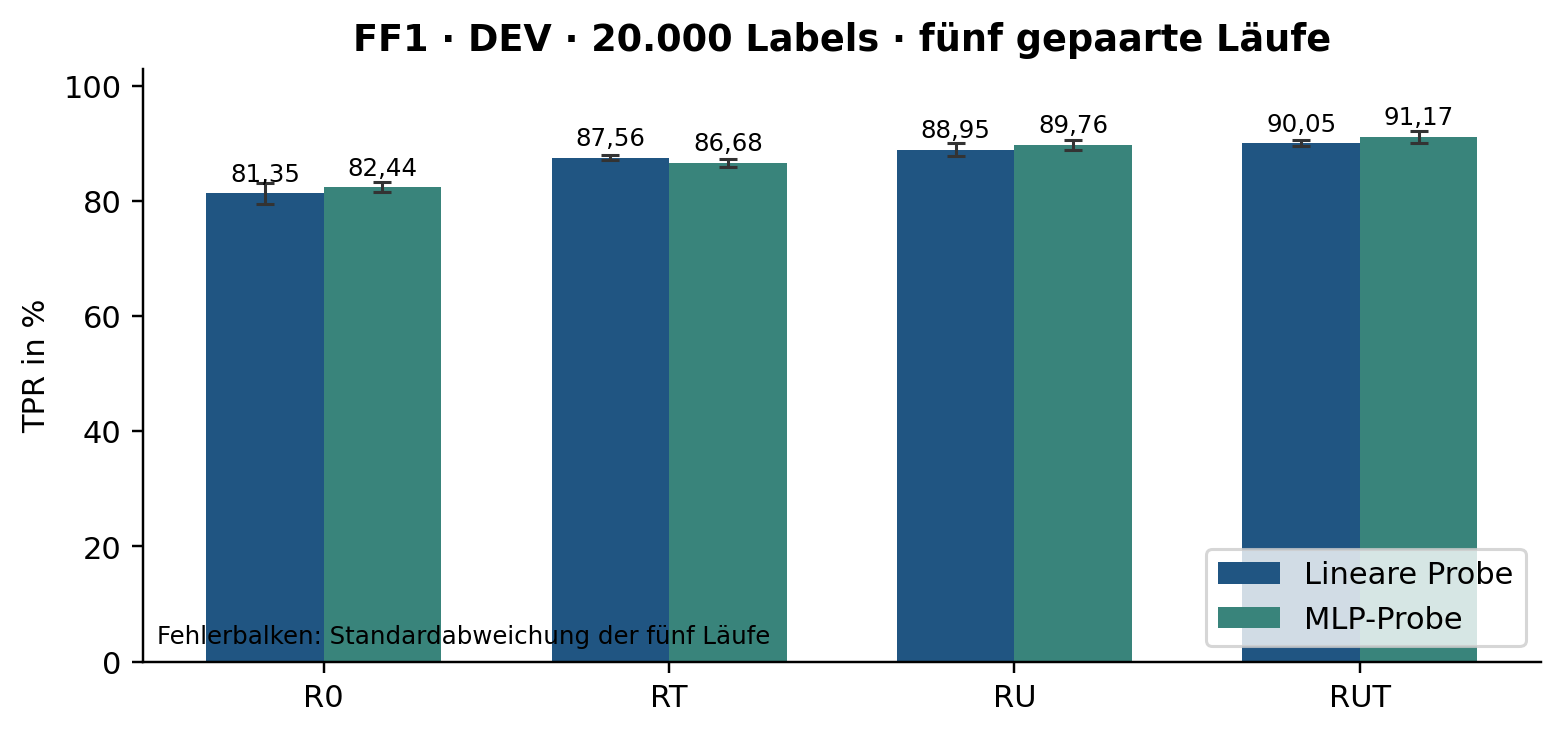
\includegraphics[width=0.82\textwidth]{Praefix/Image/06_1_FF1_ABLATION.png}
\caption{FF1: TPR der vier Repräsentationsvarianten mit linearer und MLP-Downstream-Probe.}
\label{fig:ff1_ablation}
{\footnotesize Eigene Darstellung; KI-unterstützt.}
\end{figure}

\section{FF2: Einfluss der Labelverfügbarkeit}

FF2 untersucht den Repräsentationsvergleich über sieben verschachtelte Labelbudgets von
2.000 bis 200.000 Instanzen. Die Encoder bleiben je Repräsentationszustand unverändert;
variiert wird ausschließlich die gelabelte Downstream-Supervision.

\begin{table}[H]
\centering
\caption{FF2: Mittlere FINAL-TPR der linearen Probe über die Labelbudgets.}
\label{tab:ff2_linear}
\small
\renewcommand{\arraystretch}{0.95}
\begin{tabular}{rrrrr}
\toprule
Labels & R0 & RT & RU & RUT \\
\midrule
2.000   & 51,64\% & 52,91\% & 58,62\% & 60,94\% \\
5.000   & 62,10\% & 65,07\% & 65,21\% & 67,96\% \\
10.000  & 68,00\% & 71,28\% & 71,10\% & 73,51\% \\
20.000  & 71,63\% & 75,90\% & 75,20\% & 77,73\% \\
50.000  & 75,12\% & 79,32\% & 78,97\% & 82,01\% \\
100.000 & 76,99\% & 81,04\% & 81,36\% & 84,04\% \\
200.000 & 77,92\% & 82,26\% & 83,40\% & 85,72\% \\
\bottomrule
\end{tabular}
\end{table}

Für die lineare Probe zeigt sich über das gesamte Budgetraster ein Vorteil von RUT gegenüber
R0. Die mittlere FINAL-TPR steigt für RUT von 60,94\,\% bei 2.000 Labels auf
77,73\,\% bei 20.000 und 85,72\,\% bei 200.000 Labels; R0 erreicht an denselben
Punkten 51,64\,\%, 71,63\,\% und 77,92\,\%.

Auch mit der nichtlinearen MLP-Probe bleibt dieses Rangmuster bestehen. Der Abstand zwischen
RUT und R0 beträgt bei 2.000 Labels 10,77 Prozentpunkte, bei 20.000 Labels
8,59 Prozentpunkte und bei 200.000 Labels noch 5,30 Prozentpunkte.

\begin{table}[H]
\centering
\caption{FF2: Mittlere FINAL-TPR der MLP-Probe über die Labelbudgets.}
\label{tab:ff2_mlp}
\small
\renewcommand{\arraystretch}{0.95}
\begin{tabular}{rrrrr}
\toprule
Labels & R0 & RT & RU & RUT \\
\midrule
2.000   & 42,31\% & 43,34\% & 50,30\% & 53,08\% \\
5.000   & 53,68\% & 55,44\% & 60,49\% & 63,32\% \\
10.000  & 60,94\% & 63,64\% & 67,23\% & 69,81\% \\
20.000  & 68,27\% & 72,24\% & 74,67\% & 76,86\% \\
50.000  & 78,85\% & 82,06\% & 83,63\% & 85,31\% \\
100.000 & 82,40\% & 86,33\% & 87,09\% & 89,89\% \\
200.000 & 84,95\% & 87,88\% & 88,35\% & 90,25\% \\
\bottomrule
\end{tabular}
\end{table}

Der Vorteil der task-adaptierten Repräsentation bleibt damit bei beiden
Downstream-Klassifikatoren über sämtliche untersuchten Labelbudgets bestehen. Auf DEV erreicht RUT als
ergänzende Sättigungsperspektive mit der linearen Probe 95\,\% des eigenen
200k-Niveaus bereits bei 10.000 Labels, während R0 hierfür 50.000 Labels benötigt.
Beim MLP liegen die entsprechenden B95-Punkte bei 50.000 beziehungsweise 100.000
Labels. Auf FINAL liegt B95 dagegen für R0 und RUT jeweils bei 50.000 Labels
mit der linearen Probe und bei 100.000 Labels mit dem MLP. Die frühere relative
Sättigung von RUT auf DEV überträgt sich somit nicht auf diese FINAL-Kennzahl.
Da B95 jeweils auf das eigene Endniveau einer Variante bezogen ist, wird die
absolute Performance-Suffizienz gegenüber vollständig trainierten Referenzen erst in FF3
geprüft. Zur zusätzlichen Prüfung der Label-Effizienz außerhalb des PhreshPhish-Datenbestands werden
R0 und RUT auf dem unabhängig erhobenen Phishing Website Dataset von Putra (2023)
verglichen. Auf dem zeitlich früheren Datenbestand werden identische, verschachtelte
Stichproben von 200, 500, 1.000 und 2.000 gelabelten Webseiten für zehn gepaarte
Linear-Probes verwendet und auf dem zeitlich späteren Bestand ausgewertet. Über die gesamte externe Lernkurve erreicht RUT eine mittlere AP-AULC von 91,98\,\%
gegenüber 89,45\,\% für R0. Die gepaarte Differenz beträgt +2,54 Prozentpunkte
(95\,\%-KI [2,16; 2,91], 10/10 positive Paare, $p=0{,}001953$).

\begin{table}[H]
\centering
\caption{FF2: Externe Label-Effizienz von R0 und RUT auf dem Putra-Datensatz.}
\label{tab:ff2_putra}
\small
\renewcommand{\arraystretch}{0.95}
\begin{tabular}{rrrrl}
\toprule
Labels & R0 AP & RUT AP & $\Delta$ AP & 95\,\%-KI \\
\midrule
200   & 83,91\% & 86,51\% & +2,60 pp & [1,70; 3,51] \\
500   & 88,96\% & 91,76\% & +2,79 pp & [2,22; 3,36] \\
1.000 & 91,70\% & 94,05\% & +2,35 pp & [2,02; 2,69] \\
2.000 & 93,40\% & 95,61\% & +2,21 pp & [1,85; 2,56] \\
\bottomrule
\end{tabular}
\end{table}

Die zusätzliche Zielanpassung von Quell-RUT auf dem frühen Putra-Pool verbessert
dieses Ergebnis nicht. Ihre mittlere AP-AULC fällt von 91,98\,\% auf 90,84\,\%;
die gepaarte Differenz beträgt $-1{,}14$ Prozentpunkte
(95-\%-KI [$-1{,}50$; $-0{,}78$], zehn negative Paare, $p=0{,}001953125$).
Die budgetweisen AP-Differenzen betragen bei 200, 500, 1.000 und 2.000 Labels
$-2{,}28$, $-1{,}31$, $-0{,}49$ und $-0{,}51$ Prozentpunkte.
Auch diese vier Unterschiede bleiben nach Holm-Korrektur signifikant
($p_{\mathrm{Holm}}\leq0{,}01171875$). Der Vorteil von Quell-RUT gegenüber R0
und die Verschlechterung durch eine weitere Zielanpassung betreffen verschiedene
Interventionen; der zweite Befund begrenzt eine pauschale Empfehlung wiederholten TAPT.

RUT erreicht damit an allen vier externen Labelbudgets eine höhere mittlere AP.
Sämtliche budgetweisen Vergleiche bleiben nach Holm-Korrektur signifikant
($p_{\mathrm{Holm}}=0{,}007812$). Der innerhalb von PhreshPhish beobachtete Vorteil
der task-adaptierten Repräsentation bleibt somit auch unter begrenzter gelabelter
Supervision auf dem unabhängig erhobenen Webseitenbestand bestehen. Abbildung~\ref{fig:ff2_curves} fasst abschließend die internen Lernkurven der vier
Repräsentationsvarianten zusammen. Die externe Putra-Auswertung wird aufgrund des
abweichenden Budgetrasters separat in Tabelle~\ref{tab:ff2_putra} ausgewiesen.

\begin{figure}[H]
\centering
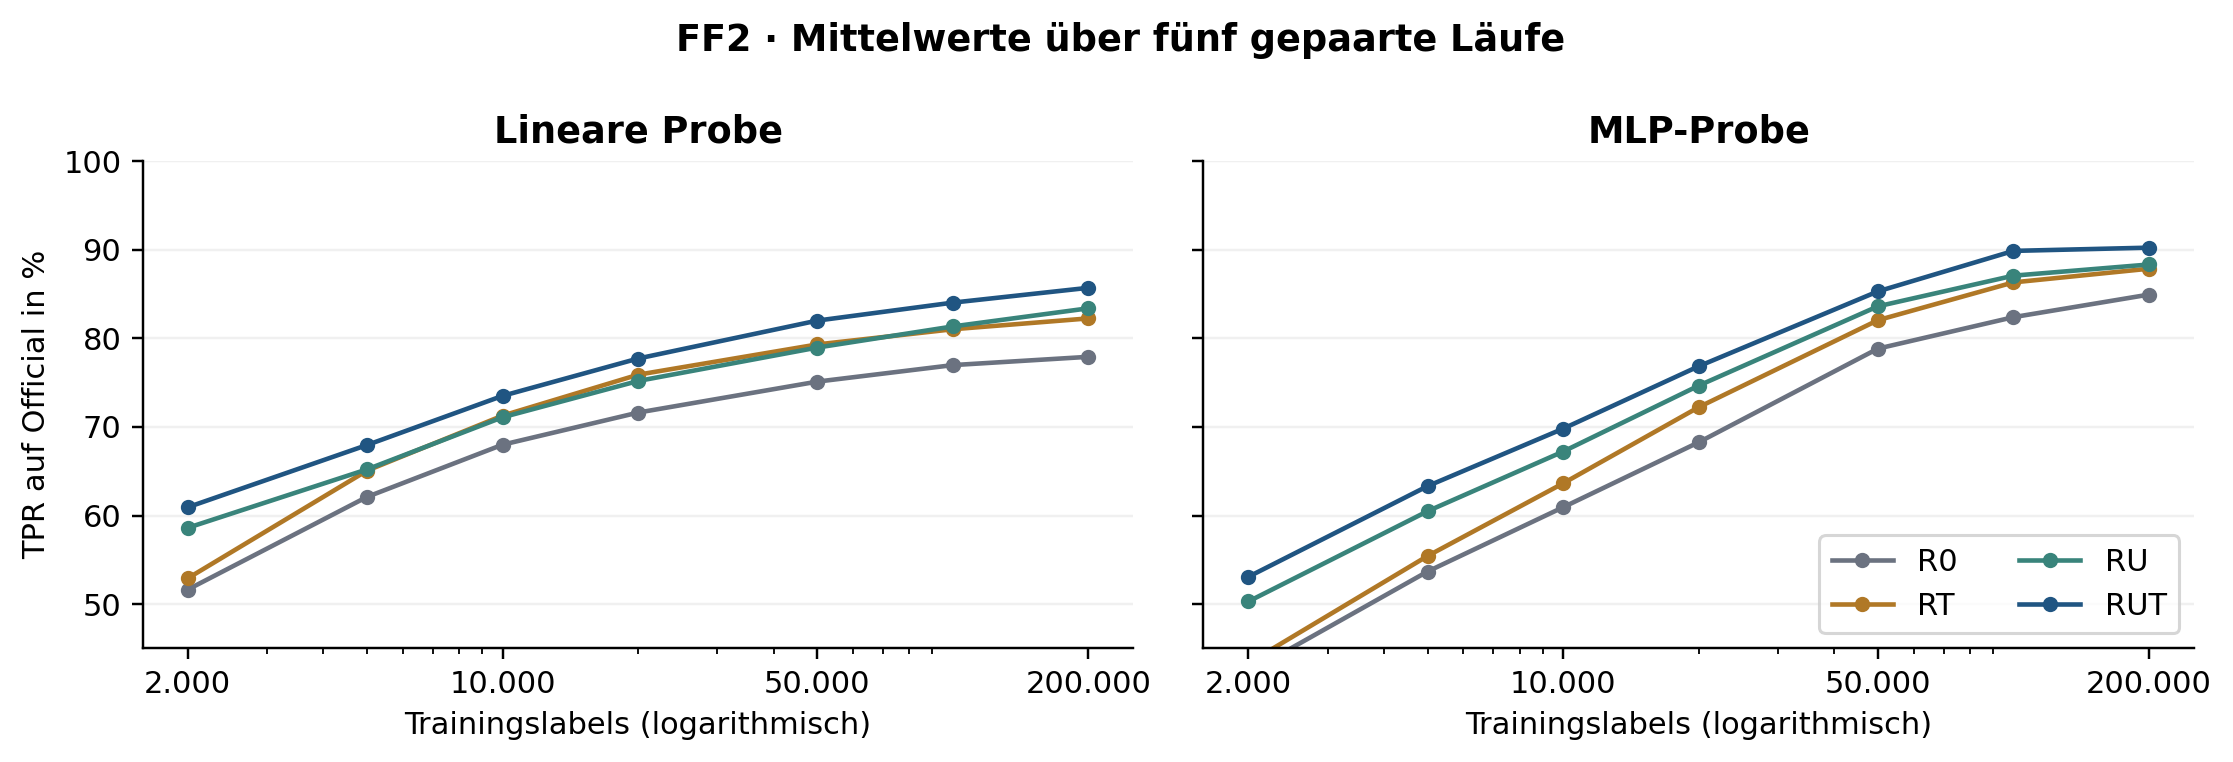
\includegraphics[width=0.78\textwidth]{Praefix/Image/06_2_FF2_LEARNING_CURVES.png}
\caption{FF2: Lernkurven der Repräsentationsvarianten über die sieben Labelbudgets mit
linearer und MLP-Probe.}
\label{fig:ff2_curves}
{\footnotesize Eigene Darstellung; KI-unterstützt.}
\end{figure}

\section{FF3: Erreichen des 200k-Referenzniveaus}

FF3 verbindet die Labelkurven mit den fünf Evaluationsbedingungen. Zunächst wird der zentrale
Vergleich zwischen RUT und R0 bei 20.000 Labels auf zehn gepaarte Wiederholungen erweitert.
Auf \nolinkurl{OFFICIAL_TEST} erreicht RUT eine TPR von 77,51\,\% gegenüber 71,43\,\% für
R0. Die mittlere gepaarte Differenz beträgt damit +6,08 Prozentpunkte
(95-\%-KI [5,38; 6,79]); alle zehn Paare zeigen einen positiven Unterschied
($p=0{,}001953$).

Auch auf Domain-OOD, Template-OOD, Domain+Template-OOD und Late Q4 liegt RUT über
R0. Die mittleren Unterschiede betragen +5,64, +6,26, +5,89 und +5,51 Prozentpunkte.
Die vier p-Werte bleiben nach Holm-Korrektur signifikant
($p_{\mathrm{Holm}}=0{,}007812$). Gleichzeitig ist die mittlere FPR von RUT in allen fünf
Bedingungen niedriger als diejenige von R0.

Anschließend wird RUT über das vollständige Budgetraster mit zwei Referenzen verglichen, die
jeweils mit 200.000 Labels trainiert wurden. Gegen R0@200k bleiben Repräsentationsformat und
Linear Probe identisch. Ein RUT-Budget wird nur dann als ausreichend bewertet, wenn die
festgelegte Nichtunterlegenheitsbedingung von einem Prozentpunkt in allen fünf
Evaluationsbedingungen erfüllt wird und die anschließende Holm-Korrektur über die sieben
Budgetentscheidungen bestehen bleibt. Abbildung~\ref{fig:ff3_heatmap} zeigt die absoluten mittleren TPR-Werte der
RUT-Repräsentation über die fünf Evaluationsbedingungen und ausgewählte Trainingsbudgets.
Die Werte steigen in allen Bedingungen mit wachsendem Labelbudget. Die Darstellung allein
legt jedoch noch keine ausreichende Budgetstufe fest; hierfür ist der statistische Vergleich mit
den beiden 200k-Referenzen maßgeblich.

\begin{figure}[!ht]
\centering
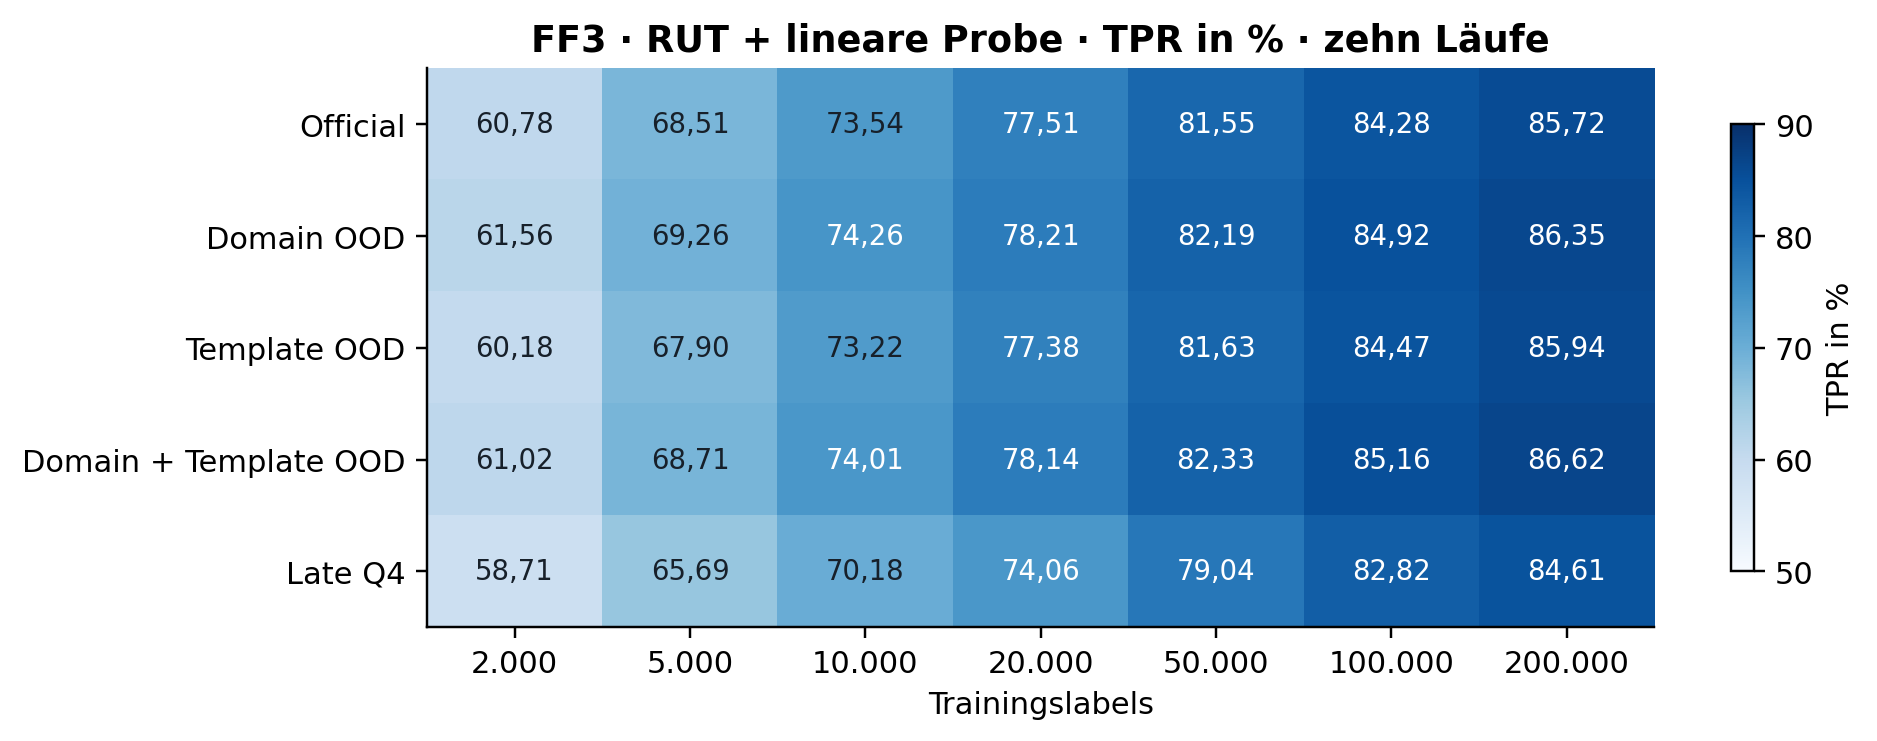
\includegraphics[width=0.76\textwidth]{Praefix/Image/FF3_RUT_TPR_Heatmap.png}
\caption{FF3: Mittlere RUT-TPR über fünf Evaluationsbedingungen und ausgewählte Labelbudgets, N10-Mittelwerte.}
\label{fig:ff3_heatmap}
{\footnotesize Eigene Darstellung; KI-unterstützt.}
\end{figure}

Gegen R0@200k reichen 20.000 Labels nach dieser Entscheidungsregel noch nicht aus. Der
ungünstigste mittlere TPR-Abstand tritt auf Late Q4 auf und beträgt $-1{,}37$
Prozentpunkte. Mit 50.000 Labels wird die Nichtunterlegenheitsbedingung dagegen in allen fünf
Bedingungen erfüllt; die korrigierte Entscheidung bleibt nach Holm signifikant
($p_{\mathrm{Holm}}=0{,}006836$). Die mittlere TPR von RUT50k liegt dabei in allen fünf
Bedingungen um +3,24 bis +3,62 Prozentpunkte über R0@200k. Gleichzeitig fällt die mittlere
realisierte FPR um 0,079 bis 0,180 Prozentpunkte niedriger aus. Als zweite Referenz dient die unabhängig trainierte TF-IDF/XGBoost-Pipeline mit 200.000
Labels. Tabelle~\ref{tab:ff3_xgb} zeigt die Ergebnisse für die beiden RUT-Budgets von 20.000
und 50.000 Labels. Bereits RUT20k erreicht in allen fünf Bedingungen mindestens die mittlere
XGBoost-TPR und zugleich eine niedrigere mittlere FPR. Der kleinste TPR-Vorsprung beträgt
auf Late Q4 allerdings nur +0,09 Prozentpunkte.

Die fünf einzelnen Nichtunterlegenheitstests für RUT20k erfüllen jeweils die
1-pp-Bedingung, die gemeinsame Budgetentscheidung erreicht nach der Holm-Korrektur über
alle sieben getesteten Budgets jedoch nicht das festgelegte Signifikanzniveau
($p_{\mathrm{Holm}}=0{,}173233$). RUT20k übertrifft XGBoost@200k damit deskriptiv in allen
fünf betrachteten Bedingungen, reicht für die strengere statistische Budgetentscheidung jedoch
nicht aus.

\begin{table}[htbp]
\centering
\caption{FF3: RUT bei 20k und 50k Labels gegenüber TF-IDF/XGBoost@200k, N10-Mittelwerte.}
\label{tab:ff3_xgb}
\small
\begin{tabular}{lrrrrrr}
\toprule
 & \multicolumn{2}{c}{XGB@200k} & \multicolumn{2}{c}{RUT20k} & \multicolumn{2}{c}{RUT50k} \\
Bedingung & TPR & FPR & TPR & FPR & TPR & FPR \\
\midrule
Official & 76,96\,\% & 0,618\,\% & 77,51\,\% & 0,520\,\% & 81,55\,\% & 0,537\,\% \\
Domain-OOD & 76,98\,\% & 1,219\,\% & 78,21\,\% & 0,951\,\% & 82,19\,\% & 0,979\,\% \\
Template-OOD & 76,75\,\% & 0,604\,\% & 77,38\,\% & 0,516\,\% & 81,63\,\% & 0,533\,\% \\
Domain+Template & 76,75\,\% & 1,186\,\% & 78,14\,\% & 0,938\,\% & 82,33\,\% & 0,966\,\% \\
Late Q4 & 73,97\,\% & 1,127\,\% & 74,06\,\% & 0,681\,\% & 79,04\,\% & 0,728\,\% \\
\bottomrule
\end{tabular}
\end{table}

Mit 50.000 Labels wird die Nichtunterlegenheitsbedingung gegenüber XGBoost@200k in allen
fünf Bedingungen erfüllt. Der gemeinsame p-Wert beträgt $2{,}561\times10^{-6}$ und nach
Holm-Korrektur $1{,}281\times10^{-5}$. Die mittlere TPR von RUT50k liegt je nach Bedingung
um +4,59 bis +5,58 Prozentpunkte höher, während gleichzeitig eine um 0,071 bis
0,398 Prozentpunkte niedrigere FPR erreicht wird.

50.000 Labels sind damit die kleinste untersuchte RUT-Stufe, die die festgelegte
Nichtunterlegenheitsbedingung sowohl gegenüber R0@200k als auch gegenüber
TF-IDF/XGBoost@200k über alle fünf Evaluationsbedingungen erfüllt. Gegenüber einem
Labelbudget von 200.000 Instanzen entspricht dies einer Reduktion der gelabelten
Downstream-Trainingsmenge um 75\,\%. Der vorausgehende TAPT-Schritt auf 200.000
ungelabelten Webseiten bleibt davon unberührt.

Die ergänzende Sensitivitätsanalyse mit TPR-Margen von 0,0, 0,5, 1,0 und 2,0
Prozentpunkten bestätigt die Stabilität dieser Budgetentscheidung. In allen vier Fällen bleiben
50.000 Labels die kleinste RUT-Stufe, die die jeweilige Testentscheidung gegenüber beiden
200k-Referenzen erfüllt. Auch ohne zugelassenen TPR-Nachteil ($\Delta=0{,}0$ pp) bleibt
RUT50k gegenüber R0@200k ($p_{\mathrm{Holm}}=0{,}006836$) und
TF-IDF/XGBoost@200k ($p_{\mathrm{Holm}}=6{,}286\times10^{-5}$) statistisch gestützt.
RUT20k reicht gegenüber R0@200k selbst bei einer auf 2,0 Prozentpunkte erweiterten Marge
nicht aus ($p_{\mathrm{Holm}}=0{,}593750$); gegenüber XGBoost@200k wird 20k erst bei
dieser 2-pp-Marge statistisch gestützt ($p_{\mathrm{Holm}}=0{,}008464$). Die gemeinsame
50k-Entscheidung bleibt damit über den untersuchten Margenbereich von 0 bis 2
Prozentpunkten unverändert.

Abbildung~\ref{fig:ff3_cross} stellt für beide Referenzen jeweils den ungünstigsten mittleren
TPR-Abstand über die fünf Evaluationsbedingungen dar. Bei 20.000 Labels liegt RUT gegenüber
XGBoost bereits knapp oberhalb der Null-Linie, gegenüber R0@200k jedoch noch unter der
festgelegten Marge. Ab 50.000 Labels sind die mittleren Abstände zu beiden Referenzen in allen
Bedingungen positiv.

\begin{figure}[!ht]
\centering
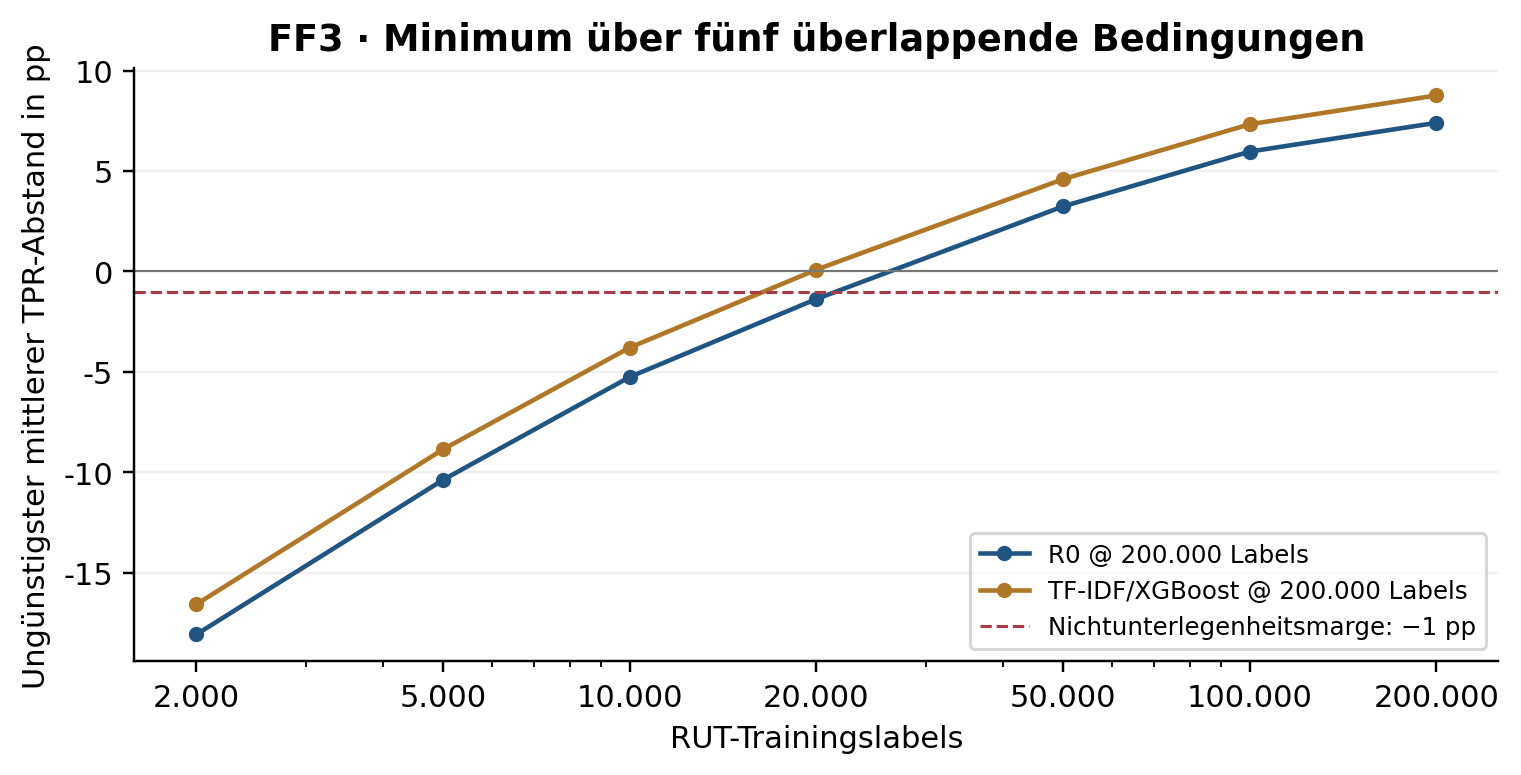
\includegraphics[width=0.80\textwidth]{Praefix/Image/FF3_Worst_Case_Gaps.png}
\caption{FF3: Schlechtester mittlerer TPR-Abstand von RUT gegenüber R0@200k und TF-IDF/XGBoost@200k über die fünf Evaluationsbedingungen.}
\label{fig:ff3_cross}
{\footnotesize Eigene Darstellung; KI-unterstützt.}
\end{figure}

\section{FF4: Inkrementeller Systembeitrag und URL-first-Verarbeitung}

FF4 untersucht den zusätzlichen Beitrag der einzelnen Systembestandteile. Hierfür wird RUT
als gemeinsame Repräsentationsbasis verwendet und auf getrennten Development-Daten eine
Folge von vier Varianten verglichen: URL-only (P0), URL+Text mit gleichgewichteter Fusion
(P1), URL+Text+DOM mit gleichgewichteter Fusion (P2) und dieselben drei Modalitäten mit
lernbarem Gating (P3). Alle Varianten erhalten innerhalb einer Replikation dieselben
20.000 Labels und werden über zehn gepaarte Wiederholungen verglichen. CAL und FINAL
werden für diese Analyse nicht verwendet.

Die mittlere TPR steigt entlang dieser Varianten von 87,932\,\% auf 93,116\,\%, 93,844\,\%
und schließlich 94,420\,\%. Den größten zusätzlichen Beitrag liefert der HTML-Text:
$P_1-P_0$ beträgt +5,184 Prozentpunkte (95-\%-KI [4,324; 6,044], 10/10 positive Paare).
Durch den DOM-Zweig steigt die TPR um weitere +0,728 Prozentpunkte
(95-\%-KI [0,305; 1,151], 10/10 positive Paare). Der Übergang von gleichgewichteter zu
lernbarer Gating-Fusion erhöht sie um weitere +0,576 Prozentpunkte
(95-\%-KI [0,226; 0,926], 9/10 positive Paare). Alle drei Vergleiche bleiben nach der
gemeinsamen Holm-Korrektur signifikant
($p_{\mathrm{Holm}}=0{,}00585938$). Die realisierte \nolinkurl{ENG_META}-FPR steigt entlang
der Varianten leicht von 0,400\,\% auf 0,616\,\%; gleichzeitig sinkt FPR@TPR90 von
0,528\,\% auf 0,260\,\%.

Die Komponentenablation wurde nach Festlegung der finalen Architektur ergänzend durchgeführt
und diente nicht zu deren nachträglicher Auswahl. Sie zeigt jedoch, dass jeder der drei
hinzugefügten Bestandteile im festgelegten Vergleich einen positiven zusätzlichen Beitrag leistet.
Passend dazu erreicht die bereits eingefrorene Gated-TRI-Konfiguration auch auf FINAL in allen
fünf Bedingungen eine höhere TPR als die gleichgewichtete Fusion. Auf
\nolinkurl{OFFICIAL_TEST} steigt die TPR von 95,65\,\% auf 96,12\,\%; in den vier
zusätzlichen Bedingungen beträgt der Unterschied 0,38 bis 0,54 Prozentpunkte. Für die Systemperspektive wird anschließend das eingefrorene TRI-Vollsystem mit der bereits vor
dem FINAL-Zugriff festgelegten URL-first-Kaskade verglichen. Auf \nolinkurl{OFFICIAL_TEST}
erreicht TRI Full 96,12\,\% TPR bei 0,666\,\% FPR, die Kaskade 95,77\,\% TPR bei
0,680\,\% FPR. Die eingefrorene Routingkonfiguration eskaliert 14,93\,\% der Webseiten;
für 85,07\,\% wird die Entscheidung bereits nach der URL-Stufe abgeschlossen. Im
In-Memory-Benchmark sinkt die Median-Latenz von 30,18 auf 11,95 ms und der Durchsatz
steigt von 183,2 auf 447,0 Seiten/s, entsprechend dem 2,44-Fachen.

\begin{table}[htbp]
\centering
\caption{FF4: In-Memory-Benchmark des vollständigen Systems und der eingefrorenen URL-first-Kaskade.}
\label{tab:ff4_runtime}
\small
\begin{tabular}{lrr}
\toprule
Kennzahl & TRI Full & TRI-Kaskade \\
\midrule
TPR, Official & 96,12\,\% & 95,77\,\% \\
FPR, Official & 0,666\,\% & 0,680\,\% \\
Eskalation, Official & 100,00\,\% & 14,93\,\% \\
\addlinespace
Median-Latenz, DEV, Batch 1 & 30,18 ms & 11,95 ms \\
95. Perzentil, DEV, Batch 1 & 47,40 ms & 32,14 ms \\
Durchsatz, DEV, Batch 32 & 183,18 Seiten/s & 447,02 Seiten/s \\
Durchsatz-Standardabweichung, drei Läufe & 1,32 Seiten/s & 2,95 Seiten/s \\
Peak-VRAM, DEV, Batch 1 & 1.022,32 MiB & 966,77 MiB \\
Peak-VRAM, DEV, Batch 32 & 1.199,81 MiB & 1.051,72 MiB \\
\bottomrule
\end{tabular}
\end{table}

Der ergänzende Frontend-Vergleich untersucht anschließend eine andere Frage. TRI-Fallback
und Routinglogik bleiben gleich; lediglich die URL-Repräsentation wird zwischen
\nolinkurl{URL_BASE} und \nolinkurl{URL_TAPT} variiert. Für beide Varianten werden auf
Development dieselben zulässigen TPR-Abweichungen gegenüber dem Vollsystem verwendet.
Diese Analyse ist von der zuvor eingefrorenen Kaskadenkonfiguration mit einer Eskalationsrate
von 14,93\,\% zu unterscheiden; die absoluten Eskalationsraten beider Versuchsblöcke sind
deshalb nicht direkt miteinander vergleichbar.

Abbildung~\ref{fig:ff4_combined} fasst die beiden für FF4 zentralen Architektur- und
Ressourcenbefunde zusammen. Panel~(a) zeigt die sequenzielle Komponentenablation, Panel~(b)
die mittlere Eskalationsrate auf dem vollständigen Official-Testbestand über die
vier untersuchten TPR-Toleranzen.

\begin{figure}[!ht]
\centering
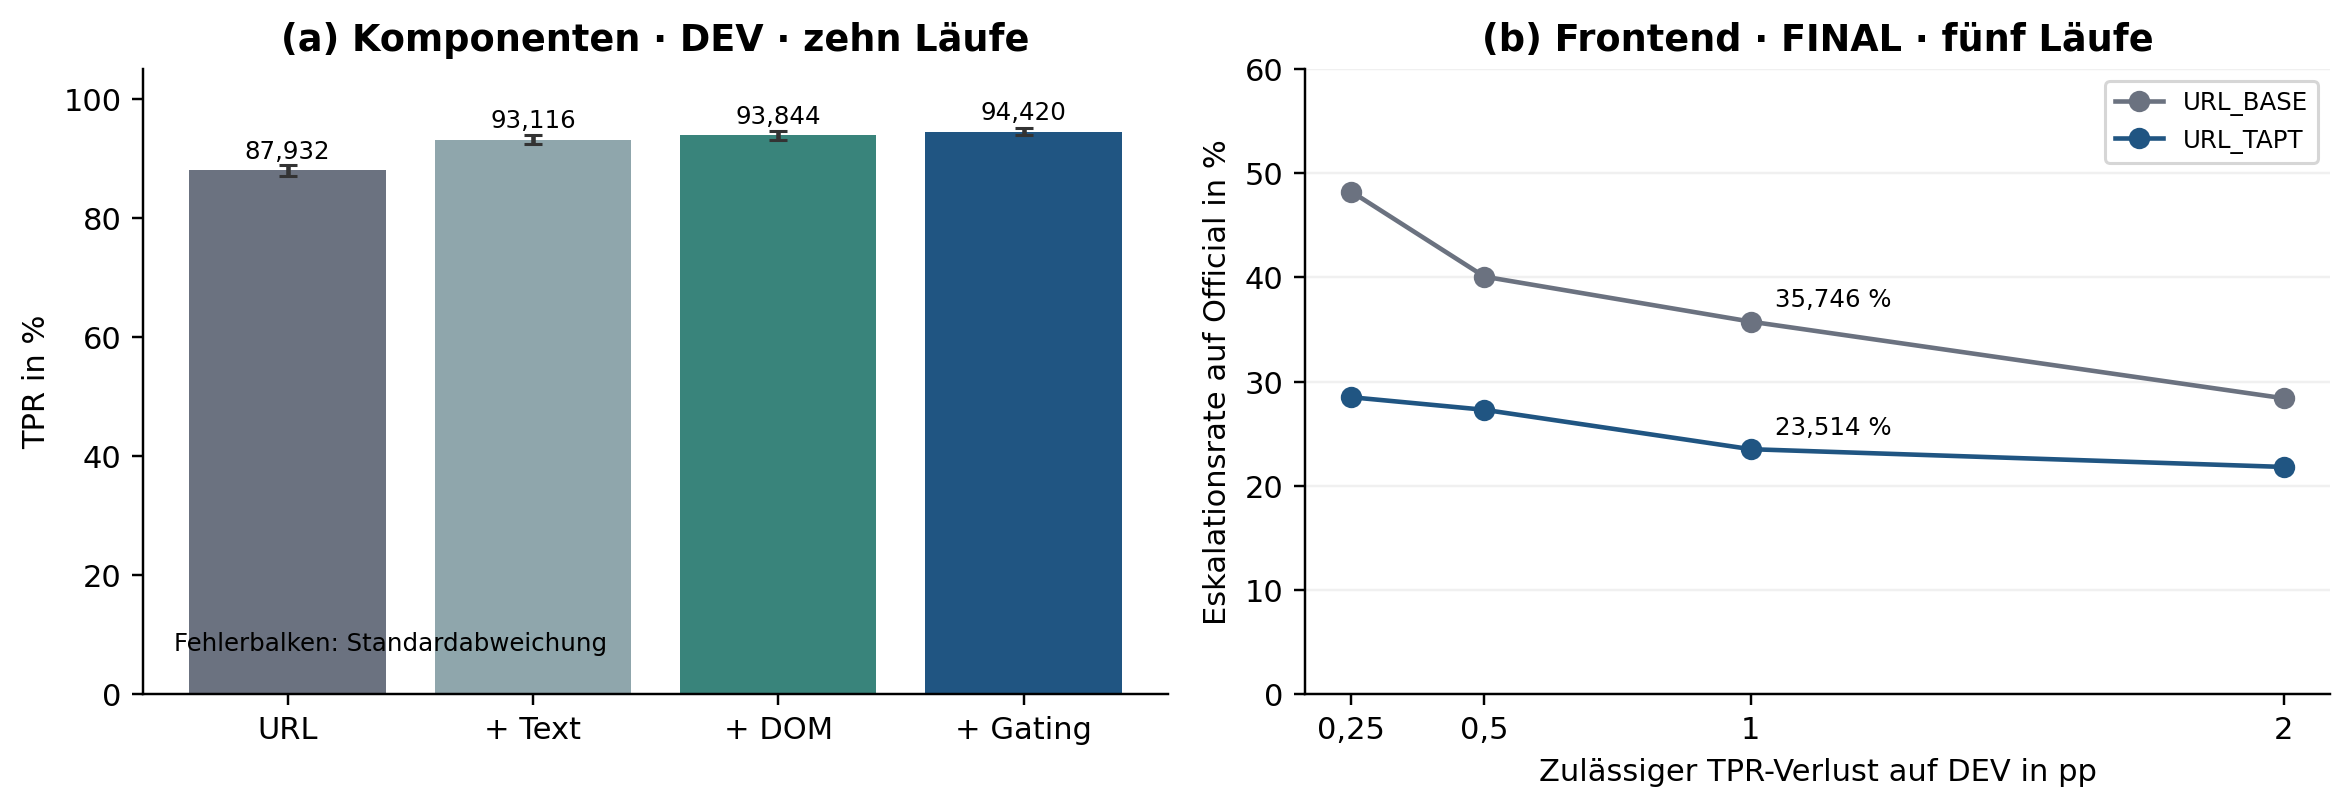
\includegraphics[width=0.90\textwidth]{Praefix/Image/FF4_Komponentenablation_Frontendvergleich.png}
\caption{FF4: Sequenzielle Komponentenablation und URL-first-Frontendvergleich von \nolinkurl{URL_BASE} und \nolinkurl{URL_TAPT}.}
\label{fig:ff4_combined}
{\footnotesize Eigene Darstellung; KI-unterstützt.}
\end{figure}

Bei der primären Toleranz von einem Prozentpunkt sinkt der ungewichtete
Szenariomittelwert der Eskalationsrate mit dem task-adaptierten URL-Frontend
von 41,125\,\% auf 28,728\,\%. Die fünf Szenarien überlappen; dieser Makromittelwert
beschreibt deshalb keine disjunkte Gesamtpopulation. Der Unterschied beträgt
12,397 Prozentpunkte. Der entsprechende Makromittelwert des Anteils früher URL-Entscheidungen beträgt
71,272\,\%. Die niedrigere Eskalationsrate von \nolinkurl{URL_TAPT} zeigt sich
in allen fünf Evaluationsbedingungen und liegt dort zwischen 10,810 und 13,438 Prozentpunkten
unter \nolinkurl{URL_BASE}. Die mittlere TPR-Abweichung vom Vollsystem beträgt
$-0{,}791$ Prozentpunkte, die mittlere FPR-Differenz $-0{,}014$ Prozentpunkte. Unter
derselben auf Development festgelegten TPR-Toleranz benötigt das task-adaptierte
URL-Frontend damit seltener die nachgelagerte vollständige multimodale Verarbeitung.

Auf dem vollständigen \nolinkurl{OFFICIAL_TEST} beträgt die mittlere Eskalationsrate
35,746\,\% für URL\_BASE und 23,514\,\% für URL\_TAPT
(Differenz $-12{,}232$ Prozentpunkte, fünf Läufe). URL\_TAPT schließt dort
76,486\,\% der Webseiten im URL-Pfad ab. Gegenüber dem Vollsystem beträgt die
TPR-Differenz $-0{,}940$ und die FPR-Differenz $+0{,}016$ Prozentpunkte.
Die niedrigere Eskalation geht somit mit einem kleinen Qualitätsverlust gegenüber
dem Vollsystem einher; die auf DEV gewählte Toleranz garantiert keine identische Test-TPR.

\section{Ergänzende Unsicherheits- und Prävalenzeinordnung}

Ergänzend zur Betriebspunktanalyse werden AP und $P_{\geq 90}$ auf dem festen
\nolinkurl{OFFICIAL_TEST} mit 1.000 stratifizierten Bootstrap-Replikationen ausgewertet.
TRI Full erreicht eine AP von 99,679\,\% mit einem 95-\%-Percentile-Intervall von
[99,659; 99,700]\,\% sowie ein $P_{\geq 90}$ von 99,714\,\%
[99,673; 99,753]\,\%. Die Kaskade erreicht eine AP von 98,539\,\%
[98,476; 98,602]\,\% und ein $P_{\geq 90}$ von 99,776\,\%
[99,742; 99,815]\,\%. Die engen Intervalle zeigen eine geringe Stichprobenunsicherheit
dieser Rankingmetriken auf dem festen Testbestand. Für die absolute Höhe precision-basierter Kennzahlen ist zusätzlich die Klassenprävalenz
relevant, also der Anteil phishingbezogener Webseiten innerhalb der Evaluationsmenge. Der
\nolinkurl{OFFICIAL_TEST} enthält 76.800 Phishing- und 91.260 Benign-Instanzen und weist
damit einen Phishing-Anteil von 45,70\,\% auf. Dies entspricht nahezu der für den regulären
PhreshPhish-Testbestand berichteten Base Rate von 46\,\%
(vgl. [Dalton et al. (2026), S. 6--7]). Zur Einordnung wird deshalb eine reine
Base-Rate-Sensitivität von $P_{\geq 90}$ berechnet. Für die ausgewählte Schwelle
werden die klassenspezifischen Scoreverteilungen konstant gehalten und ausschließlich
die angenommene Prävalenz verändert. Mit der beobachteten Precision $P_0$ und
der Testprävalenz $\pi_0=76.800/168.060$ gilt
\[
\lambda=\frac{1-P_0}{P_0}\frac{\pi_0}{1-\pi_0}
       =\frac{\mathrm{FPR}_*}{\mathrm{TPR}_*},
\qquad
\mathrm{Precision}_{\pi}=\frac{\pi}{\pi+(1-\pi)\lambda}.
\]
Hierbei kennzeichnet $*$ die für $P_{\geq 90}$ ausgewählte empirische Schwelle.
Die Umrechnung benötigt keinen Recall von exakt 90\,\%. Sie bildet einen reinen
Prior-Shift ab; Veränderungen des klassenspezifischen Fehlerverhaltens sind darin
nicht enthalten.

\begin{table}[htbp]
\centering
\caption{Base-Rate-Sensitivität von $P_{\geq 90}$.}
\label{tab:base_rate_sensitivity}
\small
\begin{tabular}{lrr}
\toprule
Phishing-Base-Rate & TRI Full & TRI-Kaskade \\
\midrule
45,70\,\% & 99,714\,\% & 99,776\,\% \\
5\,\%     & 95,62\,\%  & 96,54\,\% \\
1\,\%     & 80,74\,\%  & 84,27\,\% \\
\bottomrule
\end{tabular}
\end{table}

Die rechnerischen Werte bei 1\,\% Base Rate betragen 80,74\,\% für TRI Full und
84,27\,\% für die Kaskade. Sie sind keine Messungen auf einem neu erhobenen Bestand
mit dieser Prävalenz. Ein direkter Vergleich mit separat konstruierten
PhreshPhish-Benchmarks wäre wegen unterschiedlicher Testzusammensetzung und nicht
abgeglichener Metrikimplementierung nicht belastbar. Die primäre Systembewertung
stützt sich weiterhin auf TPR und FPR am festgelegten Betriebspunkt.

\chapter{Diskussion und Schlussbetrachtung}

Das Kapitel beantwortet die vier Forschungsfragen, grenzt die Aussagekraft der internen und
externen Ergebnisse ein und leitet daraus ein betriebliches Einsatz- und Pilotkonzept ab.


\section{Interpretation und Beantwortung der Forschungsfragen}

\textbf{FF1 -- task-adaptive Repräsentationsanpassung.}
R0 bildet bereits einen allgemein selbstüberwacht vortrainierten Ausgangspunkt. Der in dieser
Arbeit gemessene Effekt beschreibt daher den zusätzlichen Nutzen der task-adaptiven
Weiteranpassung. RU und RT verbessern die Downstream-Leistung gegenüber R0, während
RUT mit beiden Probes die höchste mittlere TPR erreicht. Der N10-Vergleich bestätigt diesen
Vorteil auf FINAL: Auf \nolinkurl{OFFICIAL_TEST} liegt RUT bei 20.000 Labels um
+6,08 Prozentpunkte über R0; in den vier zusätzlichen Evaluationsbedingungen beträgt der
Unterschied +5,51 bis +6,26 Prozentpunkte und bleibt nach Holm-Korrektur signifikant.

Damit zeigt sich ein zusätzlicher Repräsentationsnutzen der Anpassung auf dem ungelabelten
Webseitenpool, obwohl die Ausgangsencoder bereits selbstüberwacht vortrainiert sind.
Die in Kapitel 3 dargestellten spezialisierten URL-Repräsentationsverfahren verdeutlichen
die Relevanz einer domänennäheren Repräsentationsbildung für URL-basierte
Sicherheitsaufgaben (vgl. [Maneriker et al. (2021), PDF-S. 1--2]; [Wang et al. (2023), Abstract, o.\,S.]; [Li et al. (2025), S. 1--2 und 12]).
Die vorliegende Untersuchung betrachtet diesen Zusammenhang für die zusätzliche
task-adaptive Anpassung zweier Informationszweige innerhalb desselben Versuchsprotokolls.

Die faktorielle Betrachtung zeigt zugleich, dass sich die einzelnen Adaptationsgewinne nicht
vollständig addieren. Die Interaktion beträgt $-5{,}10$ Prozentpunkte für die lineare und
$-2{,}83$ Prozentpunkte für die MLP-Probe. URL- und HTML-Text-TAPT liefern damit jeweils
einen positiven Beitrag, weisen bei gemeinsamer Anpassung jedoch eine teilweise Überlappung
ihrer Effekte auf. RUT bleibt dennoch die Variante mit der höchsten absoluten
Downstream-Leistung.

Der vorgelagerte kontrastive Versuchsblock ist davon getrennt zu interpretieren. Die
getesteten kontrastiven Varianten lagen unter der damaligen Basis- und MLM-Konfiguration,
wurden jedoch nicht unter dem finalen R0/RU/RT/RUT-Protokoll erneut trainiert. Daraus
lässt sich keine allgemeine Aussage über kontrastives Lernen gegenüber MLM-basiertem
TAPT ableiten.


\textbf{FF2 -- Einfluss der Labelverfügbarkeit.}
Der RUT-Vorteil bleibt über alle untersuchten internen Labelbudgets von 2.000 bis
200.000 Instanzen bestehen. Bei kleineren Trainingsmengen ist der Abstand zu R0 besonders
ausgeprägt; mit zunehmender gelabelter Supervision verringert er sich, ohne vollständig zu
verschwinden. Die task-adaptive Repräsentationsanpassung verbessert damit nicht nur einen
einzelnen Betriebspunkt, sondern den Verlauf der gesamten Lernkurve.

Für die Einordnung ist die Trennung der beiden Lernphasen relevant. Der TAPT-Schritt
verwendet den 200.000 Instanzen umfassenden SSL-Pool ohne Downstream-Labels. Erst im
anschließenden Klassifikationstraining wird der Umfang der verfügbaren gelabelten Supervision
variiert. Die Sensitivität gegenüber reduziertem gelabeltem Trainingsumfang wird auch für
spezialisierte URL-Repräsentationen als relevante Evaluationsdimension betrachtet
(vgl. [Li et al. (2025), S. 12]). Die B95-Auswertung weist ausschließlich auf DEV auf eine frühere relative Sättigung von RUT hin; auf FINAL erreichen R0 und RUT das jeweilige relative Ziel bei denselben geprüften Budgets.
Da sich B95 jeweils auf das eigene 200k-Endniveau einer Variante bezieht, beantwortet diese
Kennzahl jedoch nicht, ob ein reduziertes RUT-Budget auch das absolute Niveau einer
vollständig trainierten Referenz erreicht. Diese Frage wird durch FF3 gesondert geprüft.

Die externe Evaluation auf dem Phishing Website Dataset von Putra (2023) erweitert diese
Einordnung über den PhreshPhish-Datenbestand hinaus. Bei identischen gelabelten
Zielinstanzen erreicht RUT über die vier Budgets von 200 bis 2.000 Webseiten eine um
2,54 Prozentpunkte höhere AP-AULC als R0 (95\,\%-KI [2,16; 2,91], 10/10 positive
Paare, $p=0{,}001953$). Auch die vier einzelnen Budgetvergleiche fallen mit
AP-Vorteilen zwischen +2,21 und +2,79 Prozentpunkten zugunsten von RUT aus und bleiben
nach Holm-Korrektur signifikant. Der Nutzen der task-adaptierten Repräsentation zeigt sich damit nicht ausschließlich innerhalb
der ursprünglichen PhreshPhish-Lernkurve. Im untersuchten externen Datenbestand bildet RUT
auch bei begrenzter neuer gelabelter Supervision die günstigere Ausgangsbasis für die
Downstream-Klassifikation. Der Befund stützt damit die Annahme, dass eine zuvor auf
ungelabelten Webseitendaten angepasste Repräsentation die spätere Anpassung an eine neue
Zielumgebung erleichtern kann.


Die ergänzende Putra-Zielanpassung verschlechtert dagegen die AP-AULC um
1,14 Prozentpunkte. Mehr selbstüberwachtes Vortraining führt folglich in diesem
Protokoll nicht zwangsläufig zu besseren Repräsentationen. Der Versuch isoliert
weder die Ursache der Verschlechterung noch eine optimale Adaptationsstärke;
insbesondere Lernrate, Trainingsdauer und Korpusgröße wurden hier nicht systematisch variiert.

\textbf{FF3 -- Erreichen des Referenzniveaus bei reduziertem Labelbudget.}
Die formale Budgetanalyse zeigt, dass 50.000 Labels die kleinste untersuchte RUT-Stufe
sind, die das festgelegte Vergleichsniveau gegenüber R0@200k über alle fünf
Evaluationsbedingungen einschließlich Holm-Korrektur erreicht. Die mittlere TPR von
RUT50k liegt dabei um +3,24 bis +3,62 Prozentpunkte über R0@200k; zugleich fällt die
realisierte FPR niedriger aus.

Auch gegenüber TF-IDF/XGBoost@200k ist 50.000 die kleinste statistisch gestützte
Budgetstufe. RUT20k liegt zwar bereits in allen fünf Bedingungen mindestens auf der
mittleren XGBoost-TPR und weist gleichzeitig eine niedrigere mittlere FPR auf, besteht
jedoch die Korrektur über das vollständige Budgetraster nicht. Mit RUT50k beträgt der
TPR-Abstand zu XGBoost je nach Evaluationsbedingung +4,59 bis +5,58 Prozentpunkte.
Da sich bei diesem Vergleich sowohl Repräsentation als auch Klassifikator ändern, dient
XGBoost als zusätzliche Referenz für das erreichbare Leistungsniveau und nicht als isolierter
Nachweis eines TAPT-Effekts.

Im untersuchten Linear-Probe-Protokoll reichen damit 50.000 gelabelte Instanzen aus, um
das festgelegte Leistungsniveau beider mit 200.000 Labels trainierten Referenzen zu erreichen.
Bezogen auf die Downstream-Supervision entspricht dies einer Reduktion um 75\,\%. Der
vorausgehende TAPT-Schritt auf dem vollständigen ungelabelten Webseitenpool bleibt davon
unberührt. Die Margensensitivität bestätigt die 50k-Entscheidung zusätzlich über den
untersuchten Bereich von 0 bis 2 Prozentpunkten. Die zusätzlichen internen Evaluationsbedingungen zeigen, dass diese Relation nicht auf den
vollständigen Finalbestand beschränkt ist. Dies ist insbesondere vor dem in Kapitel 3
diskutierten Problem datensatzabhängiger Evaluationsresultate relevant
(vgl. [Rashid et al. (2024), Abstract, o.\,S.]; [Dalton et al. (2026), S. 5--6]). Die Domain-,
Template- und Zeitbedingungen sind jedoch nicht als kausale Einzeltests verschiedener Formen
von Distribution Shift zu verstehen. Sie prüfen, ob die in FF1 und FF2 identifizierten
Leistungsrelationen unter veränderter Zusammensetzung der Testdaten erhalten bleiben.

Die realisierte FPR liegt insbesondere auf den domainbezogenen Teilmengen teilweise oberhalb
des auf CAL angestrebten Betriebspunkts. Eine stabile Rangfolge der Modelle bedeutet daher
nicht, dass ein einmal kalibrierter Schwellenwert unter jeder Datenverteilung dieselbe FPR
erzeugt. Repräsentationsrobustheit und Betriebspunktkalibration sind entsprechend als getrennte
Fragestellungen zu behandeln. Auch die ergänzende Prävalenzanalyse aus Abschnitt 6.6 betrifft eine andere Eigenschaft der
Evaluation. Unter konstant gehaltenem klassenspezifischem Fehlerverhalten sinkt
$P_{\geq 90}$ bei einer rechnerischen Phishing-Base-Rate von 1\,\% auf 80,74\,\%
für TRI Full beziehungsweise 84,27\,\% für die Kaskade. Die Analyse verdeutlicht damit
die Abhängigkeit precision-basierter Kennzahlen von der Klassenprävalenz.


\textbf{FF4 -- multimodale Systemkomponenten und URL-first-Verarbeitung.}
Die sequenzielle Komponentenablation zeigt positive zusätzliche Beiträge aller drei
Erweiterungsschritte. Den größten Zuwachs liefert HTML-Text mit +5,184 Prozentpunkten
TPR gegenüber URL-only. Der DOM-Zweig erhöht die TPR anschließend um weitere
+0,728 Prozentpunkte und das lernbare Gating um +0,576 Prozentpunkte. Alle drei
benachbarten Vergleiche bleiben nach Holm-Korrektur signifikant.

Die Ergebnisse zeigen damit für das implementierte System, dass die in Kapitel 3 diskutierten
textuellen und strukturellen Webseiteninformationen über die URL hinaus zusätzliche
Klassifikationsinformation bereitstellen können (vgl. [Aljofey et al. (2022), S. 1--2 und 13]; [Yoon et al. (2024), S. 13 und 15]). Gleichzeitig unterscheiden sich ihre marginalen Beiträge:
Der HTML-Text erzeugt den größten zusätzlichen Effekt, während DOM und Gating kleinere,
aber statistisch gestützte Verbesserungen liefern. TRI Full erreicht auf \nolinkurl{OFFICIAL_TEST} 96,12\,\% TPR bei 0,666\,\% FPR und
bildet die leistungsstärkste Variante des implementierten Gesamtsystems. Die
URL-first-Kaskade ergänzt diese Architektur um eine gestufte Verarbeitung. In der
eingefrorenen Routingkonfiguration werden 14,93\,\% der Webseiten an den vollständigen
TRI-Pfad eskaliert; die TPR beträgt 95,77\,\%. Gleichzeitig sinkt die Median-Latenz von
30,18 auf 11,95\,ms und der gemessene In-Memory-Durchsatz steigt von 183,2 auf
447,0 Seiten pro Sekunde. Die Kaskade realisiert damit das in Kapitel 3 aufgegriffene
Prinzip einer mehrstufigen Verarbeitung, ohne den multimodalen Pfad für unsichere Fälle
aufzugeben (vgl. [Liu et al. (2021), Abstract, o.\,S.]). Der Frontend-Vergleich verbindet schließlich Repräsentations- und Systemebene. Bei derselben
auf Development festgelegten TPR-Toleranz von einem Prozentpunkt sinkt die mittlere
Eskalationsrate auf \nolinkurl{OFFICIAL_TEST} von 35,746\,\% mit URL\_BASE
auf 23,514\,\% mit URL\_TAPT (fünf Läufe).
Die task-adaptierte URL-Repräsentation ermöglicht innerhalb dieses Routingprotokolls damit
häufiger eine Entscheidung in der ersten Verarbeitungsstufe. Der Repräsentationsvorteil wirkt
sich folglich nicht nur auf die Klassifikationsleistung eines einzelnen Modells, sondern auch
auf die Verarbeitungstiefe des Gesamtsystems aus.

Die zentrale Forschungsfrage wird damit auf drei Ebenen beantwortet: zusätzlicher
Repräsentationsnutzen durch TAPT, geringerer gelabelter Trainingsbedarf im Probe-Protokoll
und eine steuerbare Verarbeitungstiefe des darauf aufbauenden multimodalen Systems.


\section{Limitationen und Aussagegrenzen}

Die internen Generalisierungsanalysen beruhen auf demselben PhreshPhish-Data-Freeze.
Der ergänzende Integritätsaudit schließt für die prüfbaren OOD-Instanzen exakte
Überschneidungen der Domains beziehungsweise Template-Hashes mit SUP, DEV, CAL und
dem SSL/TAPT-Pool aus. Semantisch ähnliche Webseiten, Near-Duplicates und fehlende
Domainwerte werden dadurch jedoch nicht vollständig erfasst. Die zusätzliche Evaluation auf dem unabhängig erhobenen Putra-Datensatz erweitert die
Untersuchung um eine externe Datenquelle. Sie bestätigt den RUT--R0-Vorteil für die
Label-Effizienz mit einer linearen Downstream-Probe, umfasst jedoch nur einen einzelnen
zusätzlichen Webseitenbestand. Die Übertragbarkeit auf weitere Erhebungszeiträume,
Datenquellen und Zielumgebungen bleibt daher offen. Zudem adressiert diese externe
Prüfung die Repräsentations- und Label-Effizienz und nicht das vollständige multimodale
TRI-System oder die URL-first-Kaskade. N5 und N10 variieren die Auswahl der gelabelten Trainingsinstanzen und das
Downstream-Training, während die zugrunde liegenden TAPT-Checkpoints unverändert bleiben.
Die berichteten Unsicherheiten erfassen damit nicht die Variation vollständig neu ausgeführter
selbstüberwachter Vortrainingsläufe.

Die Reduktion von 200.000 auf 50.000 Instanzen betrifft ausschließlich die gelabelte
Downstream-Supervision. Für TAPT werden weiterhin 200.000 Webseiten verarbeitet. Der
PhreshPhish-Bestand stellt grundsätzlich Klasseninformationen bereit; diese werden im
SSL-Pool für das selbstüberwachte Training technisch nicht verwendet und erst für die
späteren Downstream-Experimente wieder zugeordnet. Die Untersuchung quantifiziert damit
den methodischen Nutzen einer ohne Downstream-Labels durchgeführten
Repräsentationsanpassung, nicht den betrieblichen Prozess der erstmaligen Erhebung und
Annotation der Daten. Die verwendete 1-pp-Nichtunterlegenheitsmarge ist eine analytische Entscheidungsschwelle
und keine betrieblich validierte Servicegrenze. Die ergänzende Margensensitivität reduziert
die Abhängigkeit der zentralen FF3-Entscheidung von dieser konkreten Festlegung, ersetzt
jedoch keine anwendungsspezifische Festlegung zulässiger Qualitätsverluste.

Die Klassenbalance der Budgetstichproben wird anhand bereits vorhandener Poollabels
hergestellt. Die Budgetanalyse simuliert daher begrenzte gelabelte Trainingsmengen,
aber keinen vollständig budgetierten Annotationsprozess. Labels für Development,
Kalibration und Evaluation sowie die Information zur klassenweisen Auswahl sind in
den 50.000 Trainingslabels nicht enthalten. Eine betriebliche Einsparung von 75\,\%
des gesamten Annotationsaufwands lässt sich daraus nicht ableiten.

Die fünf internen Testszenarien überlappen; ihre Ergebnisse sind keine fünf
unabhängigen Replikationen. Exakte Sign-Flip-p-Werte beziehen sich auf die vollständige
Enumeration der Vorzeichen, setzen für ihre inferenzielle Interpretation aber eine
entsprechende Symmetrie beziehungsweise Austauschbarkeit der Paardifferenzen voraus.
Mit zehn Replikationen ist diese Annahme nur eingeschränkt prüfbar. Die nachträglichen
Welch-Vergleiche mit XGBoost sind ergänzende Evidenz auf derselben Testpopulation,
keine unabhängige Bestätigung. Ein gespeicherter Analyseplan nach früherem FINAL-Zugriff
ersetzt keine prospektive Vorregistrierung auf einem unberührten Testset.

Die Putra-Erhebungen enden 2023 und liegen damit vor dem verwendeten PhreshPhish-Bestand
aus 2025. Der interne frühe/späte Putra-Schnitt schützt vor direkter Nutzung seiner
Testinstanzen im Zieltraining; die Gesamtauswertung ist jedoch kein prospektiver
Nachweis für zukünftige Angriffe. Eine mögliche Überschneidung mit den ursprünglichen
allgemeinen BERT-/RoBERTa-Vortrainingskorpora wurde nicht überprüft.

Weitere Grenzen betreffen die Eingabeverarbeitung. Der HTML-Textencoder verarbeitet maximal
256 Tokens und erfasst daher nicht notwendigerweise den vollständigen HTML-Inhalt. Der
DOM-Zweig basiert auf einer statischen Rekonstruktion des gespeicherten HTML und nicht auf
einem browsergerenderten Laufzeit-DOM. Die gemessenen Latenz-, Durchsatz- und
Peak-VRAM-Werte gelten ausschließlich für den In-Memory-Modellpfad ohne Netzwerkzugriffe,
Rendering, Datenträger-I/O und vorgelagertes HTML-Parsing.


\section{Betriebliches Einsatzkonzept und Handlungsempfehlung}
\label{sec:betriebskonzept}

\textbf{Einsatzaufgabe und Verantwortlichkeit.}
Konzipiert wird die Vorprüfung verdächtiger Webseiten für die Sicherheitseinheit eines
Kreditinstituts oder dessen IT-Dienstleister. Aus URL, gesichertem HTML und Meldekontext
entsteht ein Klassifikationshinweis mit Modellversion und Schwellenentscheidung für die
fachliche Bearbeitung. Tatsächliche Abläufe, Meldevolumina und Ressourcen der Volksbank
wurden nicht erhoben; der folgende Prozess ist eine eigene Konzeption.

Die technische Vorfilterung großer Ereignismengen für die anschließende menschliche Analyse
wird auch in NIST SP 800-61r3 empfohlen (vgl. [Nelson et al. (2025), S. 25]).
Für die Priorisierung und Validierung sind dort zudem Auswirkungen, Dringlichkeit und
weiterer Fallkontext maßgeblich (vgl. [Nelson et al. (2025), S. 26--27]).
Für den vorliegenden Entwurf folgt daraus eine unterstützende Rolle des Klassifikators:
Die Sicherheitseinheit verantwortet die Fallbewertung und Folgemaßnahmen. Ein hoher
Modellscore allein beschreibt weder den betrieblichen Schaden noch eine kalibrierte
Phishingwahrscheinlichkeit. Automatische Sperrungen sind deshalb kein Bestandteil dieses Konzepts.

Isolierte Erfassung, Netzwerkabruf, Ticketschnittstelle und Prüfoberfläche sind erforderliche
Erweiterungen des Prototyps. Die Eingaben müssen den untersuchten URL-/HTML-/DOM-Daten
entsprechen. Nicht auswertbare Seiten werden gesondert fachlich geklärt. Modellnegative
Seiten erhalten keine Freigabe als sicher. Relevanter Kontext, etwa eine berichtete
Zugangsdatenpreisgabe, kann unabhängig vom Modell eine sofortige Prüfung erfordern.

\begin{figure}[H]
\centering
% Eigene betriebliche Konzeption; KI-unterstuetzt. Keine implementierte Prozessmessung.
\begin{tikzpicture}[
  box/.style={draw=black!55,rounded corners=2pt,align=center,font=\small,
    text width=11.6cm,inner sep=6pt,minimum height=.7cm},
  flow/.style={-{Stealth[length=2mm]},thick},node distance=5mm]
\node[box] (in) {\textbf{Eingang und Aufbereitung}\par
Meldung mit URL und Fallkontext; isolierte Erfassung von HTML/DOM};
\node[box,below=of in,fill=black!7] (model) {\textbf{Gemessener Modellpfad}\par
TRI Full oder URL-first-Kaskade; eingefrorene Modell- und Schwellenversion};
\node[box,below=of model] (review) {\textbf{Prüfsteuerung}\par
Modellalarme und relevante Kontextfälle; Stichprobe modellnegativer Fälle;\par
nicht auswertbare Eingaben separat zur Prüfung};
\node[box,below=of review] (human) {\textbf{Fachliche Entscheidung}\par
Sicherheitseinheit bestätigt Befund und entscheidet über Folgemaßnahmen};
\node[box,below=of human] (learn) {\textbf{Dokumentation und Verbesserung}\par
Geprüfte Labels, Prüfzeit und Fehlerarten; getrennte Entwicklung und Kalibration};
\draw[flow] (in)--node[right,font=\scriptsize]{auswertbar}(model);
\draw[flow] (in.west) -- ++(-.7,0) |- (review.west);
\node[font=\scriptsize,rotate=90] at ($(in.west)!0.5!(review.west)+(-.95,0)$) {nicht auswertbar};
\draw[flow] (model)--(review);
\draw[flow] (review)--(human);
\draw[flow] (human)--(learn);
\end{tikzpicture}

\caption{Konzipierte Einbettung der Webseitenklassifikation in die fachliche Fallprüfung. Nur der grau hinterlegte Modellpfad wurde experimentell untersucht.}
\label{fig:betriebsprozess}
{\footnotesize Eigene Darstellung; KI-unterstützt.}
\end{figure}

\textbf{Modellwahl nach tatsächlichem Engpass.}
Tabelle~\ref{tab:business_model_choice} vergleicht das mit 200.000 Labels trainierte
TRI-System, seine Kaskade und seinen separat gemessenen URL-Zweig.

\begin{table}[H]
\centering
\caption{Gemessene Alternativen und daraus abgeleitete Einsatzentscheidung. TPR/FPR: FINAL; Durchsatz: DEV-In-Memory-Benchmark auf Tesla T4.}
\label{tab:business_model_choice}
\small
\begin{tabular}{lrrrp{5.0cm}}
\toprule
Variante & TPR & FPR & Seiten/s & Konzeptionelle Einordnung \\
\midrule
URL-Pfad & 93,16\,\% & 0,682\,\% & 865,9 & Höchster Durchsatz; mehr übersehene Phishingfälle. \\
TRI Full & 96,12\,\% & 0,666\,\% & 183,2 & Startpunkt bei Qualitätsvorrang und ausreichender Rechenkapazität. \\
TRI-Kaskade & 95,77\,\% & 0,680\,\% & 447,0 & Option bei nachgewiesenem Rechenengpass und akzeptiertem Qualitätsverlust. \\
\bottomrule
\end{tabular}
\end{table}

Bei begrenztem Pilotumfang sprechen höhere TPR und niedrigere FPR für TRI Full.
Die Kaskade erhöht den gemessenen Durchsatz um den Faktor 2,44, erzeugt aber zusätzliche
Fehlalarme und übersehene Phishingfälle. Als Größenordnung entsprechen 10.000 Seiten
beim gemessenen mittleren Durchsatz 54,59 Sekunden für TRI Full und 22,37 Sekunden für
die Kaskade: 32,22 Sekunden Differenz. Diese DEV-Benchmark-Referenz umfasst weder
die gesamte Bearbeitungskette noch eine auf andere Prävalenzen angepasste Laufzeit.
Der Geschwindigkeitsvorteil ist deshalb mit tatsächlichem Eingang, Hardware und Wartezeiten abzuwägen.

\textbf{Prüfmenge und Qualitätsfolgen.}
Die Szenarien aus Abschnitt~\ref{sec:betriebspunkt_szenarien} machen die nachgelagerte
Aufgabe greifbar. Bei 10.000 auswertbaren Seiten und angenommenen 1\,\% Phishing liefert
TRI Full rund 162 Modellalarme: etwa 96 erkannte Phishingfälle und 66 Fehlalarme;
rund vier Phishingfälle bleiben modellnegativ. Die Kaskade erzeugt rechnerisch 1,41
zusätzliche Fehlalarme und 0,35 zusätzliche übersehene Phishingfälle je 10.000 Seiten.
Der schnellere URL-Pfad übersieht bei derselben Annahme 6,84 statt 3,88 Phishingfälle.
Eine kleinere Alarmmenge kann somit auch durch schlechtere Erkennung entstehen.

Werden alle Modellalarme geprüft, beschreibt $A_{\pi}$ zunächst nur diesen Teil der
menschlichen Prüfmenge. Bei einer im Pilot zu messenden mittleren Bearbeitungszeit
$t_A$ in Minuten beträgt der entsprechende Aufwand $A_{\pi}t_A/60$ Stunden.
Kontextfälle, nicht auswertbare Seiten, Negativstichproben und Folgemaßnahmen kommen hinzu.
Eine Personal- oder Kosteneinsparung wurde nicht gemessen. Ebenso wenig sind die rund
660 zusätzlichen Modellpfade der Kaskade im 1-\%-Szenario 660 menschliche Prüffälle.
Der beiliegende Betriebsrechner trennt diese Größen und erlaubt eigene, kenntlich
gemachte Volumen-, Prävalenz- und Zeitannahmen.

\textbf{Datenstrategie bei begrenzter Annotation.}
Die Label-Effizienz liefert eine zweite, von der Laufzeit getrennte Handlungsempfehlung:
Eine vorhandene RUT-Repräsentation ist ein begründeter Ausgangspunkt für begrenztes
gelabeltes Nachtraining. Intern erreicht RUT50k das festgelegte Referenzniveau der
200k-Verfahren; extern erzielt RUT auf Putra über 200 bis 2.000 Ziel-Labels einen
AP-AULC-Vorteil von 2,54 Prozentpunkten. Der interne 50k-Nachweis gilt allerdings für
lineare Probes auf eingefrorenen Repräsentationen. Die in diesem Einsatzkonzept
verwendeten Full-/Kaskadenwerte stammen aus einem mit 200k Labels trainierten System.
Eine Kombination von 50k Trainingslabels mit dessen 96,12\,\% TPR wurde nicht nachgewiesen.

Die 75\,\% Reduktion betrifft zudem ausschließlich Downstream-Trainingslabels;
Entwicklung, Kalibration, Evaluation, Datenerhebung und TAPT bleiben eigene
Aufwandspositionen. Für einen neuen Betrieb sollte zunächst eine Lernkurve mit geprüftem
Zielmaterial erhoben werden. Zusätzliche Ziel-TAPT wäre eine separat zu bewertende Option,
da sie im ergänzenden Putra-Versuch die AP-AULC um 1,14 Prozentpunkte verschlechterte.
Geprüfte Fälle dürfen erst nach Dokumentation und Rollentrennung für spätere Modellstände
genutzt werden. Derselbe Fall darf nicht zugleich Nachtraining und dessen Erfolgskontrolle dienen.

\textbf{Pilotierung und messbare Freigabeentscheidung.}
Als nächster Entwicklungsschritt wird ein Parallelbetrieb vorgeschlagen, bei dem der
bestehende fachliche Prüfprozess die Fallentscheidung weiterhin trifft. TRI Full und
Kaskade bewerten dieselben neu eingehenden auswertbaren Fälle. Modellstand, Schwellen,
Routing und die Erfolgskriterien werden vor der Pilotbewertung festgelegt.
Kalibration auf neuem Zielmaterial und anschließende zeitlich getrennte Bewertung
ermöglichen eine Überprüfung des tatsächlichen Betriebspunkts. Die fachlichen Labels
sollten möglichst ohne Kenntnis der Modellentscheidung vergeben werden.

\begin{table}[H]
\centering
\caption{Vorgeschlagene Prüfkriterien für die betriebliche Weiterentwicklung; noch keine gemessene Freigabe.}
\label{tab:business_pilot}
\small
\begin{tabular}{p{3.0cm}p{10.9cm}}
\toprule
Prüfdimension & Zu erfassender Nachweis und Entscheidung \\
\midrule
Datenabdeckung & Anteil auswertbarer Fälle und Ursachen fehlender Eingaben; gesonderte Bearbeitung der Ausfälle muss möglich sein. \\
Detektionsqualität & TPR, FPR und Precision mit Unsicherheit auf unabhängig geprüften Fällen; die Sicherheitseinheit legt akzeptable Grenzen vor Auswertung fest. Die CAL-Ziel-FPR von 0,5\,\% ist keine bereits bestätigte Betriebsgrenze. \\
Prüfkapazität & Alarme, Kontextfälle, Negativstichprobe, mittlere Prüfzeit und Rückstand; tatsächlicher Aufwand muss in die vereinbarte Kapazität passen. \\
Verarbeitung & Gesamtlatenz einschließlich Erfassung, Durchsatz und Modellrouting; Kaskade nur bei relevantem Ressourcenvorteil und vertretbaren zusätzlichen Fehlern. \\
Änderungskontrolle & Bei Qualitätsverschlechterung zuerst Datenabdeckung und Betriebspunkt prüfen; Rekalibration und Nachtraining getrennt bewerten und an zeitlich späteren Fällen erneut prüfen. \\
\bottomrule
\end{tabular}
\end{table}

Werden nur Modellalarme gelabelt, bleiben übersehene Phishingfälle unbekannt. Der Pilot
benötigt daher entweder eine vollständige fachliche Referenzbewertung oder zusätzlich
eine Zufallsstichprobe modellnegativer Fälle mit dokumentierten Auswahlwahrscheinlichkeiten.
Bei ungleichen Prüfanteilen müssen Prävalenz und Fehlerraten entsprechend gewichtet werden.
Das Konzept verbindet damit die vorhandenen Ergebnisse mit einer überprüfbaren
Einführungsentscheidung: Qualitätsvorrang im ersten Pilot, Kaskade bei nachgewiesenem
Ressourcenbedarf und gezielte Labelverwendung für spätere Modellanpassungen.


\clearpage
\section{Fazit und Ausblick}

Die zusätzliche task-adaptive Anpassung bereits vortrainierter URL- und HTML-Text-Encoder
verbessert im untersuchten Protokoll die Phishing-Erkennung. RUT erreicht bei 20.000 Labels
auf dem vollständigen FINAL-Bestand eine um 6,08 Prozentpunkte höhere mittlere TPR als R0.
Die Adaptationseffekte überlagern sich teilweise.

50.000 Labels bilden die kleinste geprüfte RUT-Stufe, welche die festgelegte
Nichtunterlegenheitsentscheidung gegenüber R0@200k und TF-IDF/XGBoost@200k in allen fünf
Evaluationsbedingungen erfüllt. Die Reduktion um 75\,\% betrifft ausschließlich die gelabelte
Downstream-Trainingsmenge des Linear-Probe-Protokolls; die anschließenden
Full-/Kaskadenwerte beruhen auf 200.000 Trainingslabels. Auf dem externen Putra-Bestand verbessert Quell-RUT die AP-AULC
gegenüber R0 um 2,54 Prozentpunkte; die zusätzliche Putra-Anpassung verschlechtert sie
hingegen um 1,14 Prozentpunkte. Weitere selbstüberwachte Anpassung ist damit kein
allgemeines Verbesserungsversprechen.

HTML-Text, DOM und Gating liefern im sequenziellen DEV-Vergleich jeweils einen zusätzlichen
Beitrag. TRI Full erreicht auf FINAL 96,12\,\% TPR bei 0,666\,\% FPR. Die URL-first-Kaskade
eskaliert 14,93\,\% der Fälle und erreicht 95,77\,\% TPR. Ihr DEV-In-Memory-Durchsatz
ist 2,44-mal so hoch wie der des Vollsystems; die Messung umfasst nicht die gesamte Verarbeitungskette.


Das betriebliche Einsatzkonzept sieht TRI Full zur unterstützenden Webseitenvorprüfung
vor; die Kaskade ist bei nachgewiesenem Rechenengpass zu prüfen. Bei angenommenen
1\,\% Phishing erzeugt TRI Full je 10.000 Seiten rund 162 Modellalarme, darunter 66
Fehlalarme. Modellrouting, Alarmmenge und menschliche Prüfung bleiben getrennte Größen,
deren Übertragung der vorgeschlagene Pilot überprüfen soll.

Feste TAPT-Checkpoints, nachträgliche Analysen und der retrospektive externe Test begrenzen
die Verallgemeinerung. Ausstehend sind unabhängige Vortrainingswiederholungen, zukünftige
externe Systemtests, Kostenmessungen sowie die betriebliche Prüfung von Rekalibration
und Drift-Erkennung.

\chapter*{Literaturverzeichnis}
\markboth{Literaturverzeichnis}{Literaturverzeichnis}
\addcontentsline{toc}{chapter}{Literaturverzeichnis}
\noindent Die angegebenen Fundstellen beziehen sich auf die im jeweiligen Eintrag
ausgewiesene Fassung. PDF-S. bezeichnet die physische Seitenzählung einer unpaginierten
Quelle; o.\,S. kennzeichnet unpaginierte Webquellen.

\par\smallskip
\begin{samepage}
\noindent
Aljofey, Ali; Jiang, Qingshan; Rasool, Abdur; Chen, Hui; Liu, Wenyin;
Qu, Qiang und Wang, Yang (2022):
An effective detection approach for phishing websites using URL and HTML features.
In: \textit{Scientific Reports}, 12, Artikel 8842.
\url{https://www.nature.com/articles/s41598-022-10841-5.pdf}.
Abruf bzw. erneuter Quellenabgleich am 12.09.2026.
\par\end{samepage}
\par\smallskip
\begin{samepage}
\noindent
Anti-Phishing Working Group (APWG) (Hrsg.; 2025):
\textit{Phishing Activity Trends Report. 1st Quarter 2025}.
\url{https://docs.apwg.org/reports/apwg_trends_report_q1_2025.pdf}.
Abruf bzw. erneuter Quellenabgleich am 12.09.2026.
\par\end{samepage}
\par\smallskip
\begin{samepage}
\noindent
Arevalo, John; Solorio, Thamar; Montes-y-Gómez, Manuel und González, Fabio A. (2017):
Gated Multimodal Units for Information Fusion.
In: \textit{5th International Conference on Learning Representations (ICLR 2017),
Workshop Track}.
\url{https://arxiv.org/pdf/1702.01992}.
Abruf bzw. erneuter Quellenabgleich am 12.09.2026.
\par\end{samepage}
\par\smallskip
\begin{samepage}
\noindent
Baltrušaitis, Tadas; Ahuja, Chaitanya und Morency, Louis-Philippe (2019):
Multimodal Machine Learning: A Survey and Taxonomy.
In: \textit{IEEE Transactions on Pattern Analysis and Machine Intelligence},
41(2), S.~423--443.
\url{https://ieeexplore.ieee.org/document/8269806}.
Seitenangaben im Text beziehen sich auf die Autorenfassung mit 20 PDF-Seiten. \url{https://arxiv.org/abs/1705.09406}.
Abruf bzw. erneuter Quellenabgleich am 12.09.2026.
\par\end{samepage}
\par\smallskip
\begin{samepage}
\noindent
Bengio, Yoshua (2009):
Learning Deep Architectures for AI.
In: \textit{Foundations and Trends in Machine Learning}, 2(1), S.~1--127.
\url{https://doi.org/10.1561/2200000006}.
Abruf bzw. erneuter Quellenabgleich am 12.09.2026.
\par\end{samepage}
\par\smallskip
\begin{samepage}
\noindent
Botsch, Benny (2023):
\textit{Maschinelles Lernen -- Grundlagen und Anwendungen. Mit Beispielen in Python}.
Springer Spektrum, Berlin, Heidelberg.
ISBN 978-3-662-67277-8.
\url{https://doi.org/10.1007/978-3-662-67277-8}.
Abruf bzw. erneuter Quellenabgleich am 12.09.2026.
\par\end{samepage}
\par\smallskip
\begin{samepage}
\noindent
Chen, Ting; Kornblith, Simon; Norouzi, Mohammad und Hinton, Geoffrey (2020):
A Simple Framework for Contrastive Learning of Visual Representations.
In: \textit{Proceedings of the 37th International Conference on Machine Learning},
Proceedings of Machine Learning Research, 119, S.~1597--1607.
PMLR.
\url{https://proceedings.mlr.press/v119/chen20j/chen20j.pdf}. Seitenangaben im Text nach physischer PDF-Zählung.
Abruf bzw. erneuter Quellenabgleich am 12.09.2026.
\par\end{samepage}
\par\smallskip
\begin{samepage}
\noindent
Collobert, Ronan; Weston, Jason; Bottou, Léon; Karlen, Michael;
Kavukcuoglu, Koray und Kuksa, Pavel (2011):
Natural Language Processing (Almost) from Scratch.
In: \textit{Journal of Machine Learning Research}, 12, S.~2493--2537.
\url{https://www.jmlr.org/papers/v12/collobert11a.html}.
Abruf bzw. erneuter Quellenabgleich am 12.09.2026.
\par\end{samepage}
\par\smallskip
\begin{samepage}
\noindent
Cybenko, George (1989):
Approximation by superpositions of a sigmoidal function.
In: \textit{Mathematics of Control, Signals, and Systems},
2(4), S.~303--314.
\url{https://link.springer.com/article/10.1007/BF02551274}.
Abruf bzw. erneuter Quellenabgleich am 12.09.2026.
\par\end{samepage}
\par\smallskip
\begin{samepage}
\noindent
Dalton, Thomas; Gowda, Hemanth; Rao, Girish; Pargi, Sachin;
Hadj Khodabakhshi, Alireza; Rombs, Joseph; Jou, Stephan und Marwah, Manish (2026):
PhreshPhish: A Real-World, High-Quality, Large-Scale Phishing Website Dataset and Benchmark.
arXiv Preprint, arXiv:2507.10854v2, Fassung vom 11.02.2026.
\url{https://arxiv.org/abs/2507.10854v2}.
Abruf bzw. erneuter Quellenabgleich am 12.09.2026.
\par\end{samepage}
\par\smallskip
\begin{samepage}
\noindent
Devlin, Jacob; Chang, Ming-Wei; Lee, Kenton und Toutanova, Kristina (2019):
BERT: Pre-training of Deep Bidirectional Transformers for Language Understanding.
In: \textit{Proceedings of the 2019 Conference of the North American Chapter
of the Association for Computational Linguistics: Human Language Technologies},
Volume~1, S.~4171--4186.
Association for Computational Linguistics.
\url{https://doi.org/10.18653/v1/N19-1423}.
Abruf bzw. erneuter Quellenabgleich am 12.09.2026.
\par\end{samepage}
\par\smallskip
\begin{samepage}
\noindent
Dhamija, Rachna; Tygar, J. D. und Hearst, Marti (2006):
Why Phishing Works.
In: \textit{Proceedings of the SIGCHI Conference on Human Factors in Computing Systems
(CHI 2006)}, S.~581--590.
ACM.
\url{https://doi.org/10.1145/1124772.1124861}.
Verwendete Autorenfassung; PDF-Seitenzählung (10 Seiten). \url{https://people.eecs.berkeley.edu/~tygar/papers/Phishing/why_phishing_works.pdf}.
Abruf bzw. erneuter Quellenabgleich am 12.09.2026.
\par\end{samepage}
\par\smallskip
\begin{samepage}
\noindent
Dror, Rotem; Baumer, Gili; Bogomolov, Marina und Reichart, Roi (2017):
Replicability Analysis for Natural Language Processing:
Testing Significance with Multiple Datasets.
In: \textit{Transactions of the Association for Computational Linguistics},
5, S.~471--486.
\url{https://doi.org/10.1162/tacl_a_00074}.
Abruf bzw. erneuter Quellenabgleich am 12.09.2026.
\par\end{samepage}
\par\smallskip
\begin{samepage}
\noindent
Ericsson, Linus; Gouk, Henry; Loy, Chen Change und Hospedales, Timothy M. (2022):
Self-Supervised Representation Learning: Introduction, Advances, and Challenges.
In: \textit{IEEE Signal Processing Magazine}, 39(3), S.~42--62.
\url{https://doi.org/10.1109/MSP.2021.3134634}.
Abruf bzw. erneuter Quellenabgleich am 12.09.2026.
\par\end{samepage}
\par\smallskip
\begin{samepage}
\noindent
European Union Agency for Cybersecurity (ENISA) (Hrsg.; 2020):
\textit{How to set up CSIRT and SOC. Good Practice Guide}.
European Union Agency for Cybersecurity.
\url{https://www.enisa.europa.eu/publications/how-to-set-up-csirt-and-soc}.
\url{https://doi.org/10.2824/056764}.
Abruf bzw. erneuter Quellenabgleich am 12.09.2026.
\par\end{samepage}
\par\smallskip
\begin{samepage}
\noindent
European Union Agency for Cybersecurity (ENISA) (Hrsg.; 2021):
\textit{Cybersecurity for SMEs -- Challenges and Recommendations}.
European Union Agency for Cybersecurity.
\url{https://www.enisa.europa.eu/publications/enisa-report-cybersecurity-for-smes}.
\url{https://doi.org/10.2824/770352}.
Abruf bzw. erneuter Quellenabgleich am 12.09.2026.
\par\end{samepage}
\par\smallskip
\begin{samepage}
\noindent
European Union Agency for Cybersecurity (ENISA) (Hrsg.; 2024):
\textit{ENISA Threat Landscape 2024}.
European Union Agency for Cybersecurity.
\url{https://www.enisa.europa.eu/publications/enisa-threat-landscape-2024}.
\url{https://doi.org/10.2824/0710888}.
Abruf bzw. erneuter Quellenabgleich am 12.09.2026.
\par\end{samepage}
\par\smallskip
\begin{samepage}
\noindent
European Union Agency for Cybersecurity (ENISA) (Hrsg.; 2025a):
\textit{ENISA Threat Landscape 2025}, Version 1.2 (Januar 2026).
European Union Agency for Cybersecurity.
\url{https://www.enisa.europa.eu/publications/enisa-threat-landscape-2025}.
\url{https://doi.org/10.2824/1946374}.
Abruf bzw. erneuter Quellenabgleich am 12.09.2026.
\par\end{samepage}
\par\smallskip
\begin{samepage}
\noindent
European Union Agency for Cybersecurity (ENISA) (Hrsg.; 2025b):
\textit{ENISA Threat Landscape: Finance Sector. January 2023 to June 2024}.
European Union Agency for Cybersecurity.
\url{https://www.enisa.europa.eu/publications/enisa-threat-landscape-finance-sector}.
\url{https://doi.org/10.2824/5410466}.
Abruf bzw. erneuter Quellenabgleich am 12.09.2026.
\par\end{samepage}
\par\smallskip
\begin{samepage}
\noindent
Gao, Tianyu; Yao, Xingcheng und Chen, Danqi (2021):
SimCSE: Simple Contrastive Learning of Sentence Embeddings.
In: \textit{Proceedings of the 2021 Conference on Empirical Methods in Natural Language Processing},
S.~6894--6910.
Association for Computational Linguistics.
\url{https://doi.org/10.18653/v1/2021.emnlp-main.552}.
Abruf bzw. erneuter Quellenabgleich am 12.09.2026.
\par\end{samepage}
\par\smallskip
\begin{samepage}
\noindent
Gui, Jie; Chen, Tuo; Zhang, Jing; Cao, Qiong; Sun, Zhenan; Luo, Hao und Tao, Dacheng (2024):
A Survey on Self-Supervised Learning: Algorithms, Applications, and Future Trends.
In: \textit{IEEE Transactions on Pattern Analysis and Machine Intelligence}, 46(12),
S.~9052--9071.
\url{https://doi.org/10.1109/TPAMI.2024.3415112}.
Verwendete paginierte Autorenfassung; Textbeleg auf S.~1. \url{https://arxiv.org/abs/2301.05712}.
Abruf bzw. erneuter Quellenabgleich am 12.09.2026.
\par\end{samepage}
\par\smallskip
\begin{samepage}
\noindent
Gururangan, Suchin; Marasović, Ana; Swayamdipta, Swabha; Lo, Kyle;
Beltagy, Iz; Downey, Doug und Smith, Noah A. (2020):
Don't Stop Pretraining: Adapt Language Models to Domains and Tasks.
In: \textit{Proceedings of the 58th Annual Meeting of the Association for Computational Linguistics},
S.~8342--8360.
Association for Computational Linguistics.
\url{https://doi.org/10.18653/v1/2020.acl-main.740}.
Abruf bzw. erneuter Quellenabgleich am 12.09.2026.
\par\end{samepage}
\par\smallskip
\begin{samepage}
\noindent
Holm, Sture (1979):
A Simple Sequentially Rejective Multiple Test Procedure.
In: \textit{Scandinavian Journal of Statistics}, 6(2), S.~65--70.
\url{https://www.jstor.org/stable/4615733}.
Abruf bzw. erneuter Quellenabgleich am 12.09.2026.
\par\end{samepage}
\par\smallskip
\begin{samepage}
\noindent
Holt, Charles A. und Sullivan, Sean P. (2023):
Permutation Tests for Experimental Data.
In: \textit{Experimental Economics}, 26(4), S.~775--812.
\url{https://doi.org/10.1007/s10683-023-09799-6}.
Abruf bzw. erneuter Quellenabgleich am 12.09.2026.
\par\end{samepage}
\par\smallskip
\begin{samepage}
\noindent
Kipf, Thomas N. und Welling, Max (2017):
Semi-Supervised Classification with Graph Convolutional Networks.
In: \textit{5th International Conference on Learning Representations (ICLR 2017)}.
\url{https://openreview.net/forum?id=SJU4ayYgl}.
Abruf bzw. erneuter Quellenabgleich am 12.09.2026.
\par\end{samepage}
\par\smallskip
\begin{samepage}
\noindent
Koh, Pang Wei; Sagawa, Shiori; Marklund, Henrik; Xie, Sang Michael;
Zhang, Marvin; Balsubramani, Akshay; Hu, Weihua; Yasunaga, Michihiro;
Phillips, Richard Lanas; Gao, Irena; Lee, Tony; David, Etienne;
Stavness, Ian; Guo, Wei; Earnshaw, Berton; Haque, Imran;
Beery, Sara M.; Leskovec, Jure; Kundaje, Anshul; Pierson, Emma;
Levine, Sergey; Finn, Chelsea und Liang, Percy (2021):
WILDS: A Benchmark of in-the-Wild Distribution Shifts.
In: \textit{Proceedings of the 38th International Conference on Machine Learning},
Proceedings of Machine Learning Research, 139, S.~5637--5664.
PMLR.
\url{https://proceedings.mlr.press/v139/koh21a.html}. Seitenangaben im Text nach physischer PDF-Zählung.
Abruf bzw. erneuter Quellenabgleich am 12.09.2026.
\par\end{samepage}
\par\smallskip
\begin{samepage}
\noindent
LeCun, Yann; Bengio, Yoshua und Hinton, Geoffrey (2015):
Deep Learning.
In: \textit{Nature}, 521, S.~436--444.
\url{https://doi.org/10.1038/nature14539}.
Abruf bzw. erneuter Quellenabgleich am 12.09.2026.
\par\end{samepage}
\par\smallskip
\begin{samepage}
\noindent
Li, Yujie; Liu, Yiwei; Li, Peiyue; Jia, Yifan und Wang, Yanbin (2025):
Continuous multi-task pre-training for malicious URL detection and webpage classification.
In: \textit{Computer Networks}, 270, Artikel 111513.
\url{https://www.sciencedirect.com/science/article/pii/S1389128625004803}.
Seitenangaben im Text beziehen sich auf Version 2 der Autorenfassung (17 Seiten). \url{https://arxiv.org/abs/2402.11495v2}.
Abruf bzw. erneuter Quellenabgleich am 12.09.2026.
\par\end{samepage}
\par\smallskip
\begin{samepage}
\noindent
Liu, Dong-Jie; Geng, Guang-Gang; Jin, Xiao-Bo und Wang, Wei (2021):
An efficient multistage phishing website detection model based on the CASE feature framework:
Aiming at the real web environment.
In: \textit{Computers \& Security}, 110, Artikel 102421.
\url{https://www.sciencedirect.com/science/article/pii/S0167404821002455}.
Textbeleg: Abstract der unpaginierten Verlags-Webfassung.
Abruf bzw. erneuter Quellenabgleich am 12.09.2026.
\par\end{samepage}
\par\smallskip
\begin{samepage}
\noindent
Liu, Yinhan; Ott, Myle; Goyal, Naman; Du, Jingfei; Joshi, Mandar;
Chen, Danqi; Levy, Omer; Lewis, Mike; Zettlemoyer, Luke und Stoyanov, Veselin (2019):
RoBERTa: A Robustly Optimized BERT Pretraining Approach.
arXiv Preprint, arXiv:1907.11692.
\url{https://arxiv.org/abs/1907.11692}.
Abruf bzw. erneuter Quellenabgleich am 12.09.2026.
\par\end{samepage}
\par\smallskip
\begin{samepage}
\noindent
Maneriker, Pranav; Stokes, Jack W.; Garcia Lazo, Edir; Carutasu, Diana;
Tajaddodianfar, Farid und Gururajan, Arun (2021):
URLTran: Improving Phishing URL Detection Using Transformers.
In: \textit{MILCOM 2021 -- 2021 IEEE Military Communications Conference (MILCOM)},
S.~197--204.
IEEE.
\url{https://ieeexplore.ieee.org/document/9653028}.
Verwendete Autorenfassung; PDF-Seitenzählung (10 Seiten). \url{https://arxiv.org/abs/2106.05256}.
Abruf bzw. erneuter Quellenabgleich am 12.09.2026.
\par\end{samepage}
\par\smallskip
\begin{samepage}
\noindent
Manning, Christopher D.; Raghavan, Prabhakar und Schütze, Hinrich (2008):
\textit{Introduction to Information Retrieval}.
Cambridge University Press, Cambridge.
ISBN 978-0-521-86571-5.
\url{https://nlp.stanford.edu/IR-book/}.
Abruf bzw. erneuter Quellenabgleich am 12.09.2026.
\par\end{samepage}
\par\smallskip
\begin{samepage}
\noindent
Mikolov, Tomas; Sutskever, Ilya; Chen, Kai; Corrado, Greg S. und Dean, Jeff (2013):
Distributed Representations of Words and Phrases and their Compositionality.
In: \textit{Advances in Neural Information Processing Systems 26},
S.~3111--3119.
\url{https://proceedings.neurips.cc/paper/2013/hash/9aa42b31882ec039965f3c4923ce901b-Abstract.html}.
Die Textbelege beziehen sich auf die PDF-interne Seitenzählung 1--9.
Abruf bzw. erneuter Quellenabgleich am 12.09.2026.
\par\end{samepage}
\par\smallskip
\begin{samepage}
\noindent
Opara, Chidimma; Chen, Yingke und Wei, Bo (2024):
Look Before You Leap: Detecting Phishing Web Pages by Exploiting Raw URL and HTML Characteristics.
In: \textit{Expert Systems with Applications}, 236, Artikel 121183.
\url{https://doi.org/10.1016/j.eswa.2023.121183}.
Abruf bzw. erneuter Quellenabgleich am 12.09.2026.
\par\end{samepage}
\par\smallskip
\begin{samepage}
\noindent
Purwanto, Rizka Widyarini; Pal, Arindam; Blair, Alan und Jha, Sanjay (2022):
PhishSim: Aiding Phishing Website Detection With a Feature-Free Tool.
In: \textit{IEEE Transactions on Information Forensics and Security},
17, S.~1497--1512.
\url{https://doi.org/10.1109/TIFS.2022.3164212}.
Abruf bzw. erneuter Quellenabgleich am 12.09.2026.
\par\end{samepage}
\par\smallskip
\begin{samepage}
\noindent
Putra, I Kadek Agus Ariesta (2023):
\textit{Phishing Website Dataset}. Version 1, veröffentlicht am 02.07.2023.
Datensatz, Zenodo. \url{https://doi.org/10.5281/zenodo.8041387}.
Abruf bzw. erneuter Quellenabgleich am 12.09.2026.
\par\end{samepage}
\par\smallskip
\begin{samepage}
\noindent
Raschka, Sebastian (2018):
Model Evaluation, Model Selection, and Algorithm Selection in Machine Learning.
arXiv Preprint, arXiv:1811.12808.
\url{https://doi.org/10.48550/arXiv.1811.12808}.
Abruf bzw. erneuter Quellenabgleich am 12.09.2026.
\par\end{samepage}
\par\smallskip
\begin{samepage}
\noindent
Rashid, Fariza; Doyle, Ben; Han, Soyeon Caren und Seneviratne, Suranga (2024):
Phishing URL detection generalisation using Unsupervised Domain Adaptation.
In: \textit{Computer Networks}, 245, Artikel 110398.
\url{https://www.sciencedirect.com/science/article/pii/S1389128624002305}.
Textbeleg: Abstract der unpaginierten Verlags-Webfassung.
Abruf bzw. erneuter Quellenabgleich am 12.09.2026.
\par\end{samepage}
\par\smallskip
\begin{samepage}
\noindent
Reddi, Vijay Janapa; Cheng, Christine; Kanter, David; Mattson, Peter;
Schmuelling, Guenther; Wu, Carole-Jean; Anderson, Brian; Breughe, Maximilien;
Charlebois, Mark; Chou, William; Chukka, Ramesh; Coleman, Cody; Davis, Sam;
Deng, Pan; Diamos, Greg; Duke, Jared; Fick, Dave; Gardner, J. Scott;
Hubara, Itay; Idgunji, Sachin; Jablin, Thomas B.; Jiao, Jeff;
St. John, Tom; Kanwar, Pankaj; Lee, David; Liao, Jeffery; Lokhmotov, Anton;
Massa, Francisco; Meng, Peng; Micikevicius, Paulius; Osborne, Colin;
Pekhimenko, Gennady; Rajan, Arun Tejusve Raghunath; Sequeira, Dilip;
Sirasao, Ashish; Sun, Fei; Tang, Hanlin; Thomson, Michael; Wei, Frank;
Wu, Ephrem; Xu, Lingjie; Yamada, Koichi; Yu, Bing; Yuan, George;
Zhong, Aaron; Zhang, Peizhao und Zhou, Yuchen (2020):
MLPerf Inference Benchmark.
In: \textit{2020 ACM/IEEE 47th Annual International Symposium on Computer Architecture (ISCA)},
S.~446--459.
IEEE.
\url{https://doi.org/10.1109/ISCA45697.2020.00045}.
Seitenangaben im Text beziehen sich auf die Autorenfassung (15 Seiten). \url{https://arxiv.org/abs/1911.02549}.
Abruf bzw. erneuter Quellenabgleich am 12.09.2026.
\par\end{samepage}
\par\smallskip
\begin{samepage}
\noindent
Reimers, Nils und Gurevych, Iryna (2017):
Reporting Score Distributions Makes a Difference:
Performance Study of LSTM-networks for Sequence Tagging.
In: \textit{Proceedings of the 2017 Conference on Empirical Methods in Natural Language Processing},
S.~338--348.
Association for Computational Linguistics.
\url{https://doi.org/10.18653/v1/D17-1035}.
Abruf bzw. erneuter Quellenabgleich am 12.09.2026.
\par\end{samepage}
\par\smallskip
\begin{samepage}
\noindent
Roh, Yuji; Heo, Geon und Whang, Steven Euijong (2021):
A Survey on Data Collection for Machine Learning:
A Big Data--AI Integration Perspective.
In: \textit{IEEE Transactions on Knowledge and Data Engineering},
33(4), S.~1328--1347.
\url{https://doi.org/10.1109/TKDE.2019.2946162}.
Verwendete paginierte Autorenfassung; Textbeleg auf S.~1. \url{https://arxiv.org/abs/1811.03402}.
Abruf bzw. erneuter Quellenabgleich am 12.09.2026.
\par\end{samepage}
\par\smallskip
\begin{samepage}
\noindent
Rumelhart, David E.; Hinton, Geoffrey E. und Williams, Ronald J. (1986):
Learning Representations by Back-Propagating Errors.
In: \textit{Nature}, 323, S.~533--536.
\url{https://doi.org/10.1038/323533a0}.
Abruf bzw. erneuter Quellenabgleich am 12.09.2026.
\par\end{samepage}
\par\smallskip
\begin{samepage}
\noindent
Saito, Takaya und Rehmsmeier, Marc (2015):
The Precision-Recall Plot Is More Informative than the ROC Plot
When Evaluating Binary Classifiers on Imbalanced Datasets.
In: \textit{PLOS ONE}, 10(3), Artikel e0118432.
\url{https://doi.org/10.1371/journal.pone.0118432}.
Abruf bzw. erneuter Quellenabgleich am 12.09.2026.
\par\end{samepage}
\par\smallskip
\begin{samepage}
\noindent
Turney, Peter D. und Pantel, Patrick (2010):
From Frequency to Meaning: Vector Space Models of Semantics.
In: \textit{Journal of Artificial Intelligence Research},
37, S.~141--188.
\url{https://doi.org/10.1613/JAIR.2934}.
Abruf bzw. erneuter Quellenabgleich am 12.09.2026.
\par\end{samepage}
\par\smallskip
\begin{samepage}
\noindent
Vaswani, Ashish; Shazeer, Noam; Parmar, Niki; Uszkoreit, Jakob;
Jones, Llion; Gomez, Aidan N.; Kaiser, Łukasz und Polosukhin, Illia (2017):
Attention Is All You Need.
In: \textit{Advances in Neural Information Processing Systems 30},
S.~5998--6008.
\url{https://proceedings.neurips.cc/paper/2017/hash/3f5ee243547dee91fbd053c1c4a845aa-Abstract.html}.
Die Textbelege beziehen sich auf die PDF-interne Seitenzählung 1--11.
Abruf bzw. erneuter Quellenabgleich am 12.09.2026.
\par\end{samepage}
\par\smallskip
\begin{samepage}
\noindent
Viola, Paul und Jones, Michael J. (2004):
Robust Real-Time Face Detection.
In: \textit{International Journal of Computer Vision},
57(2), S.~137--154.
\url{https://doi.org/10.1023/B:VISI.0000013087.49260.FB}.
Abruf bzw. erneuter Quellenabgleich am 12.09.2026.
\par\end{samepage}
\par\smallskip
\begin{samepage}
\noindent
Wang, Yanbin; Zhu, Weifan; Xu, Haitao; Qin, Zhan; Ren, Kui und Ma, Wenrui (2023):
A Large-Scale Pretrained Deep Model for Phishing URL Detection.
In: \textit{2023 IEEE International Conference on Acoustics, Speech and Signal Processing
(ICASSP)}, S.~1--5.
IEEE.
\url{https://ieeexplore.ieee.org/document/10095719}.
Inhaltlich zitiert wird der unpaginierte Abstract zum Beitrag im IEEE Resource Center. \url{https://resourcecenter.ieee.org/conferences/icassp-2023/spsicassp23vid2453}.
Abruf bzw. erneuter Quellenabgleich am 12.09.2026.
\par\end{samepage}
\par\smallskip
\begin{samepage}
\noindent
Yoon, Jun-Ho; Buu, Seok-Jun und Kim, Hae-Jung (2024):
Phishing Webpage Detection via Multi-Modal Integration of HTML DOM Graphs
and URL Features Based on Graph Convolutional and Transformer Networks.
In: \textit{Electronics}, 13(16), Artikel 3344.
\url{https://doi.org/10.3390/electronics13163344}.
Abruf bzw. erneuter Quellenabgleich am 12.09.2026.
\par\end{samepage}
\par\smallskip
\begin{samepage}
\noindent
Zhang, Yue; Hong, Jason I. und Cranor, Lorrie Faith (2007):
CANTINA: A Content-Based Approach to Detecting Phishing Web Sites.
In: \textit{Proceedings of the 16th International Conference on World Wide Web (WWW 2007)},
S.~639--648.
ACM.
\url{https://doi.org/10.1145/1242572.1242659}.
Verwendete Autorenfassung; PDF-Seitenzählung (10 Seiten). \url{https://www.cs.cmu.edu/afs/cs.cmu.edu/Web/People/jasonh/publications/www2007-cantina-final.pdf}.
Abruf bzw. erneuter Quellenabgleich am 12.09.2026.
\par\end{samepage}
\par\smallskip
\begin{samepage}
\noindent
Zhou, Pan; Yang, Wenwen; Chen, Wei; Wang, Yanfeng und Jia, Jia (2019):
Modality Attention for End-to-End Audio-Visual Speech Recognition.
In: \textit{2019 IEEE International Conference on Acoustics, Speech and Signal Processing
(ICASSP)}, S.~6565--6569.
IEEE.
\url{https://ieeexplore.ieee.org/document/8683733}.
Verwendete Autorenfassung; PDF-Seitenzählung (5 Seiten). \url{https://hcsi.cs.tsinghua.edu.cn/Paper/Paper19/ICASSP19-ZHOUPAN.pdf}.
Abruf bzw. erneuter Quellenabgleich am 12.09.2026.
\par\end{samepage}

\clearpage
\chapter*{Ehrenwörtliche Erklärung}
Hiermit erkläre ich ehrenwörtlich,
\begin{enumerate}
\item dass ich die vorliegende Arbeit mit dem Titel
\begin{quote}\textbf{Self-Supervised Learning zur Phishing-Detektion -- Konzeption, prototypische Entwicklung und Evaluation eines lernbasierten Klassifikationssystems}\end{quote}
ohne fremde Hilfe angefertigt habe,
\item dass ich alle wörtlich oder sinngemäß übernommenen Zitate aus anderen Quellen an den entsprechenden Stellen innerhalb der Arbeit eindeutig gekennzeichnet habe,
\item dass diese Arbeit noch nicht in gleicher oder ähnlicher Form sowie vollständig oder auszugsweise einer anderen Prüfungsbehörde vorgelegt wurde,
\item dass alle von mir eingereichten digitalen Versionen der Arbeit mit den eventuell ausgedruckten und eingereichten Artefakten in Papierform inhaltlich zu 100 Prozent übereinstimmen.
\end{enumerate}
Ich bin mir bewusst, dass eine falsche Erklärung rechtliche Folgen haben wird.
\vspace{2cm}

\noindent\begin{tabularx}{\textwidth}{@{}X X@{}}\hrulefill & \hrulefill\\ Ort, Datum & Unterschrift\end{tabularx}


\appendix
\chapter{Ergänzende Implementierungs- und Prüfdetails}
\label{app:repro}
\section{Implementierungsauszüge}
Die folgenden Auszüge gehören zu den in Kapitel~5 erläuterten Implementierungsschritten.
Die vollständigen Notebooks und die nachvollziehbaren Prüfskripte liegen in den digitalen
Artefakten. Kürzungen innerhalb der Ausschnitte sind keine lauffähigen Ersatzprogramme.

\par\medskip\noindent\begin{minipage}{\dimexpr\linewidth-1em\relax}
\begin{lstlisting}[language=Python,caption={Zentraler Trainingsaufbau des URL-TAPT -- gekürzter Originalausschnitt},label={lst:url_tapt}]
# KI-Unterstuetzung: siehe KI-Erklaerung der Arbeit.
def train_url_tapt(batch_size):
    seed_all(MASTER_SEED)
    urls = read_ssl_urls()  # labels are never read here

    enc = url_tok(
        urls,
        truncation=True,
        max_length=URL_MAX_LEN,
        padding=False
    )
    model = AutoModelForMaskedLM.from_pretrained(
        URL_BASE_SRC, token=HF_TOKEN, **url_kwargs
    ).to(DEVICE)

    coll = DataCollatorForLanguageModeling(
        tokenizer=url_tok,
        mlm_probability=URL_MLM_PROB
    )
    opt = torch.optim.AdamW(
        model.parameters(),
        lr=URL_TAPT_LR,
        weight_decay=URL_TAPT_WEIGHT_DECAY
    )

    total = len(dl) * URL_TAPT_EPOCHS
    sched = get_linear_schedule_with_warmup(
        opt, int(URL_TAPT_WARMUP_FRAC * total), total
    )
\end{lstlisting}
\end{minipage}\par\medskip

\par\medskip\noindent\begin{minipage}{\dimexpr\linewidth-1em\relax}
\begin{lstlisting}[language=Python,caption={Bestimmung der Development-basierten Kaskadenschwellen},label={lst:cascade_thresholds}]
# KI-Unterstuetzung: siehe KI-Erklaerung der Arbeit.
url_high = thr_fpr(
    ET["url"][yt == 0],
    .001
)

pos = np.sort(ET["url"][yt == 1])
k = max(1, int(math.floor(.01 * len(pos))))
url_low = float(
    np.nextafter(pos[k - 1], -np.inf)
)
\end{lstlisting}
\end{minipage}\par\medskip

\par\medskip\noindent\begin{minipage}{\dimexpr\linewidth-1em\relax}
\begin{lstlisting}[language=Python,caption={Routingentscheidung der URL-first-Kaskade -- gekürzter zusammenhängender Originalauszug},label={lst:cascade_route}]
# KI-Unterstuetzung: siehe KI-Erklaerung der Arbeit.
hi = us >= url_high
lo = us <= url_low
esc = ~(hi | lo)

out[hi] = 1e9
out[lo] = -1e9
\end{lstlisting}
\end{minipage}\par\medskip

\par\medskip\noindent\begin{minipage}{\dimexpr\linewidth-1em\relax}
\begin{lstlisting}[language=Python,caption={Deterministische Rangbildung für die Datenpartitionierung},label={lst:stable_rank}]
# KI-Unterstuetzung: siehe KI-Erklaerung der Arbeit.
def stable_rank(series, salt):
    return np.fromiter(
        (
            int(
                hashlib.sha256(
                    (salt + "|" + x).encode()
                ).hexdigest()[:16],
                16
            )
            for x in series.astype(str)
        ),
        dtype=np.uint64,
        count=len(series)
    )
\end{lstlisting}
\end{minipage}\par\medskip

\par\medskip\noindent\begin{minipage}{\dimexpr\linewidth-1em\relax}
\begin{lstlisting}[language=Python,caption={Aufbereitung von HTML-Text und strukturellen Webseiteninformationen -- gekürzter Originalausschnitt},label={lst:process_row}]
# KI-Unterstuetzung: siehe KI-Erklaerung der Arbeit.
def process_row(row, include_label=True):
    s, _ = clipped_html(row.get("html"))
    no_comments = COMMENT_RE.sub(" ", s)

    toks = []
    for slash, tag in TAG_RE.findall(no_comments):
        toks.append(("/" if slash else "") + normalize_tag(tag))
        if len(toks) >= STRUCT_MAX_TOKENS:
            break
    struct = " ".join(toks)

    txt = SCRIPT_STYLE_RE.sub(" ", no_comments)
    txt = TAG_STRIP_RE.sub(" ", txt)
    txt = html_std.unescape(txt)
    txt = WS_RE.sub(" ", txt).strip()[:TEXT_MAX_CHARS]

    tags, parents, depths, attrs, children, _ = parse_dom(s)
    out = {
        "text": txt,
        "html_struct": struct,
        "template_hash": hashlib.sha256(
            struct.encode("utf-8", "ignore")
        ).hexdigest(),
        "dom_tag": tags,
        "dom_parent_idx": parents,
        "dom_depth": depths,
        "dom_attr_count": attrs,
        "dom_child_count": children,
    }
    return out
\end{lstlisting}
\end{minipage}\par\medskip

\par\medskip\noindent\begin{minipage}{\dimexpr\linewidth-1em\relax}
\begin{lstlisting}[language=Python,caption={Physische Entfernung der Klassenlabels aus dem SSL-Pool},label={lst:remove_label}]
# KI-Unterstuetzung: siehe KI-Erklaerung der Arbeit.
for role, outdir in ROLE_DIRS.items():
    x = df[df._role.eq(role)].copy()
    if not len(x):
        continue

    if role == "SSL_POOL":
        x["ssl_rank"] = x["_ssl_rank"].astype(int)
        x = x.drop(columns=["label"], errors="ignore")

    x = x.drop(columns=["_role", "_ssl_rank"], errors="ignore")
    x.to_parquet(
        outdir / f"part-{counters[role]:05d}.parquet",
        index=False,
        compression="zstd"
    )
    counters[role] += 1
\end{lstlisting}
\end{minipage}\par\medskip

\par\medskip\noindent\begin{minipage}{\dimexpr\linewidth-1em\relax}
\begin{lstlisting}[language=Python,caption={Partielle Freigabe der Transformerencoder},label={lst:freeze_last}]
# KI-Unterstuetzung: siehe KI-Erklaerung der Arbeit.
def freeze_last(model, n):
    for p in model.parameters():
        p.requires_grad = False

    layers = getattr(
        getattr(model, "encoder", None),
        "layer",
        None
    )
    if layers is None:
        layers = getattr(
            getattr(model, "transformer", None),
            "layer",
            None
        )
    if layers is None:
        raise RuntimeError(type(model))

    for layer in layers[-n:]:
        for p in layer.parameters():
            p.requires_grad = True

    if getattr(model, "pooler", None) is not None:
        for p in model.pooler.parameters():
            p.requires_grad = True
\end{lstlisting}
\end{minipage}\par\medskip

\par\medskip\noindent\begin{minipage}{\dimexpr\linewidth-1em\relax}
\begin{lstlisting}[language=Python,caption={GCN-basierte Repräsentation des statischen DOM -- gekürzter Originalausschnitt},label={lst:dom_encoder}]
# KI-Unterstuetzung: siehe KI-Erklaerung der Arbeit.
class DOMEncoder(nn.Module):
    def __init__(self):
        super().__init__()
        self.tag = nn.Embedding(len(DOM_VOCAB), 96, padding_idx=PAD)
        self.depth = nn.Embedding(32, 16)
        self.attr = nn.Embedding(32, 8)
        self.child = nn.Embedding(32, 8)
        self.inp = nn.Linear(128, DOM_DIM)
        self.layers = nn.ModuleList(
            [GCNLayer(DOM_DIM) for _ in range(DOM_LAYERS)]
        )
        self.att = nn.Linear(DOM_DIM, 1)

    def nodes(self, g):
        x = self.inp(torch.cat([
            self.tag(g["tag"]), self.depth(g["depth"]),
            self.attr(g["attr"]), self.child(g["child"])
        ], 1))

        for layer in self.layers:
            x = layer(x, g["edge"])
        return x
\end{lstlisting}
\end{minipage}\par\medskip

\par\medskip\noindent\begin{minipage}{\dimexpr\linewidth-1em\relax}
\begin{lstlisting}[language=Python,caption={Rekonstruktionsverlust des DOM-SSL -- gekürzter Originalausschnitt aus dem Trainingsloop},label={lst:dom_ssl}]
# KI-Unterstuetzung: siehe KI-Erklaerung der Arbeit.
logits = m(g)
mask = g["mask"]
if mask.any():
    loss = F.cross_entropy(
        logits[mask],
        g["orig"][mask]
    )
    opt.zero_grad(set_to_none=True)
    loss.backward()
    torch.nn.utils.clip_grad_norm_(
        m.parameters(), 1
    )
    opt.step()
\end{lstlisting}
\end{minipage}\par\medskip

\par\medskip\noindent\begin{minipage}{\dimexpr\linewidth-1em\relax}
\begin{lstlisting}[language=Python,caption={Kern der multimodalen DUAL-/TRI-Fusion -- gekürzter Architekturausschnitt},label={lst:deep_fusion}]
# KI-Unterstuetzung: siehe KI-Erklaerung der Arbeit.
class DeepFusion(nn.Module):
    def __init__(self, use_dom):
        super().__init__()
        self.gate = nn.Sequential(
            nn.Linear(PROJ_DIM, 64),
            nn.GELU(),
            nn.Linear(64, 1)
        )

        nm = 3 if use_dom else 2
        self.head = nn.Sequential(
            nn.Linear(PROJ_DIM * (nm + 1), 512),
            nn.GELU(),
            nn.Dropout(.2),
            nn.Linear(512, 128),
            nn.GELU(),
            nn.Linear(128, 1)
        )

    def forward(self, u, t, g=None):
        zs = self.encode(u, t, g)
        st = torch.stack(zs, 1)
        gw = torch.softmax(self.gate(st).squeeze(-1), 1)
        weighted = (st * gw[:, :, None]).sum(1)
        main = self.head(
            torch.cat(zs + [weighted], 1)
        ).squeeze(-1)
        return main, gw
\end{lstlisting}
\end{minipage}\par\medskip

\section{Reproduktionsumfang}
Die digitale Fassung enthält die Ergebnisdateien der Primäranalysen, getrennte ergänzende
Versuchsblöcke und die beim abschließenden Review verwendeten Prüfskripte.
\nolinkurl{empirical_audit.py} rekonstruiert die aggregierten Kennzahlen und statistischen
Entscheidungen; \nolinkurl{raw_score_audit.py} prüft Vorhersagescores gegen wiedergewonnene
Testlabels, reproduziert die stratifizierten Bootstrap-Intervalle und trainiert die
externen Linear-Probes auf den gespeicherten Repräsentationen neu.

Die Neutrainings verwenden unveränderte Auswahlhashes und Modellvorgaben. Sie ersetzen
keine Wiederholung des selbstüberwachten Encodertrainings. Einzelne Rangmetriken können
bei einer erneuten Optimierung numerisch abweichen; die Differenzen zu den historischen
Exporten werden im beigefügten Prüfbericht ausgewiesen. Die Latenz- und Durchsatzprüfung
kann nur die exportierten Messaggregate, deren Rechenbeziehungen und den Messcode
nachvollziehen, da die einzelnen Zeitmessungen nicht exportiert wurden.

\end{document}
